\documentclass[openany]{book}
\usepackage[a4paper,margin=4.72cm]{geometry}

\usepackage{graphicx}
\usepackage{siunitx} 
\usepackage{natbib}
\usepackage{mathtools}
\usepackage{amssymb}
\usepackage{amsthm}
\usepackage[italian]{babel}
\usepackage{stackengine}
\usepackage{graphicx,ifthen}
\usepackage{amsmath}
\usepackage{hyperref}
\usepackage{upgreek}
\usepackage{bm}
\usepackage{braket}
\usepackage{float}
\usepackage{cancel}
\usepackage{anyfontsize}
\usepackage{scalefnt}
\usepackage{tipa}
\usepackage{multirow}
\usepackage{array}
\usepackage{makecell}
\usepackage{subcaption}
\usepackage{tikz}
\usetikzlibrary{positioning}
\usetikzlibrary{calc}
\usepackage[version = 3]{mhchem}

\newtheorem{lem}{Lemma}
\newtheorem{axiom}{Assioma}
\newtheorem{defn}{Definizione}
\newtheorem{obs}{Osservazione}
\newtheorem{ex}{Esempio}
\newtheorem{notz}{Notazione}
\newtheorem{corl}{Corollario}
\newtheorem{teo}{Teorema}
\theoremstyle{remark}
\newtheorem{caso}{Caso}

% unità di misura
\DeclareSIUnit\angstrom{\text {Å}}
\DeclareSIUnit\atm{\text {atm}}

% insiemi
\newcommand{\N}{\mathbb{N}}
\newcommand{\R}{\mathbb{R}}
\newcommand{\C}{\mathbb{C}}
\newcommand{\Z}{\mathbb{Z}}

% vettori
\newcommand{\vx}{\bm{x}}
\newcommand{\vy}{\bm{y}}
\newcommand{\vz}{\bm{z}}
\newcommand{\vq}{\bm{q}}
\newcommand{\vp}{\bm{p}}
\newcommand{\vr}{\bm{r}}
\newcommand{\vn}{\bm{n}}
\newcommand{\vm}{\bm{m}}
\newcommand{\vf}{\bm{f}}
\newcommand{\vj}{\bm{j}}
\newcommand{\vk}{\bm{k}}
\newcommand{\vv}{\bm{v}}
\newcommand{\vb}{\bm{b}}
\newcommand{\va}{\bm{a}}
\newcommand{\vl}{\bm{l}}
\newcommand{\vA}{\bm{A}}
\newcommand{\vL}{\bm{L}}
\newcommand{\vR}{\bm{R}}
\newcommand{\vP}{\bm{P}}
\newcommand{\vJ}{\bm{J}}
\newcommand{\vM}{\bm{M}}
\newcommand{\vF}{\bm{F}}
\newcommand{\vE}{\bm{E}}
\newcommand{\vB}{\bm{B}}
\newcommand{\vQ}{\bm{Q}}
\newcommand{\vH}{\bm{H}}
\newcommand{\vgamma}{\bm{\gamma}}
\newcommand{\vdelta}{\bm{\delta}}
\newcommand{\vSigma}{\bm{\Sigma}}
\newcommand{\vo}{\bm{0}}

% operatori quantistici
\newcommand{\hata}{\hat{a}}
\newcommand{\hataT}{\hat{a}^\dagger}
\newcommand{\hatd}{\hat{d}}
\newcommand{\hatdT}{\hat{d}^\dagger}
\newcommand{\hatT}{\hat{T}}
\newcommand{\hatV}{\hat{V}}
\newcommand{\hatPi}{\hat{\Pi}}
\newcommand{\hatpi}{\hat{\pi}}
\newcommand{\hatphi}{\hat{\phi}}
\newcommand{\hatphid}{\hat{\phi}^\dagger}
\newcommand{\hatR}{\hat{R}}
\newcommand{\hatb}{\hat{b}}
\newcommand{\hatbT}{\hat{b}^\dagger}
\newcommand{\hatx}{\hat{x}}
\newcommand{\hatp}{\hat{p}}
\newcommand{\hatq}{\hat{q}}
\newcommand{\hatH}{\hat{H}}
\newcommand{\hath}{\hat{h}}
\newcommand{\hatz}{\hat{z}}
\newcommand{\hatr}{\hat{r}}
\newcommand{\hatS}{\hat{S}}
\newcommand{\hatO}{\hat{O}}
\newcommand{\hatL}{\hat{L}}
\newcommand{\hatU}{\hat{U}}
\newcommand{\hatQ}{\hat{Q}}
\newcommand{\hatA}{\hat{A}}
\newcommand{\hatB}{\hat{B}}
\newcommand{\hatC}{\hat{C}}
\newcommand{\hatCT}{\hat{C}^\dagger}
\newcommand{\hatD}{\hat{D}}
\newcommand{\hatP}{\hat{P}}
\newcommand{\hatPT}{\hat{P}^\dagger}
\newcommand{\hatE}{\hat{E}}
\newcommand{\hatJ}{\hat{J}}
\newcommand{\hatN}{\hat{N}}
\newcommand{\hatn}{\hat{n}}
\newcommand{\hatf}{\hat{f}}
\newcommand{\hatg}{\hat{g}}
\newcommand{\hatUT}{\hat{U}(t)}
\newcommand{\hatheta}{\hat{\theta}}
\newcommand{\hatfH}{\hat{\mathcal{H}}}
\newcommand{\upa}{\uparrow}
\newcommand{\doa}{\downarrow}

% operatori matematici
\newcommand{\mybraket}[2]{\langle #1 | #2 \rangle}
\newcommand{\mybrakett}[3]{\langle #1 | #2 | #3 \rangle}
\newcommand{\nsum}{\sum\nolimits}
\newcommand{\sump}{\sideset{}{'}\sum}
\newcommand{\nsump}[1]{\sideset{}{'_{#1}}\sum\nolimits}
\newcommand{\nprod}{\prod\nolimits}
\newcommand{\p}{\partial}
\newcommand{\vmedio}[1]{\langle #1 \rangle}
\newcommand{\bigvmedio}[1]{\left\langle #1 \right\rangle}
\newcommand{\comm}[2]{[#1,#2]}
\newcommand{\acomm}[2]{\{#1,#2\}}
\newcommand{\dg}{\dagger}
\newcommand{\diag}[1]{\mathrm{diag}(#1)}

% quantità
\newcommand{\action}{\mathcal{A}}
\newcommand{\dL}{\mathcal{L}}
\newcommand{\MI}{\mathbb{I}}

\newcommand{\ko}{\ket{0}}
\newcommand{\bo}{\bra{0}}

\newcommand{\kO}{\ket{\Omega}}
\newcommand{\bO}{\bra{\Omega}}

\newcommand{\zbar}{\bar{z}}

\title{\textbf{APPUNTI DI FISICA} \\ \textbf{DELLA MATERIA CONDENSATA}}
\author{Manuel Gabriele Moretti}
\date{Marzo 2026}

\begin{document}

\maketitle
\pagenumbering{roman}
\tableofcontents
\newpage

\pagenumbering{arabic}
\chapter{Superfluidità}
L'elio $\ce{He}$ è un elemento abbastanza particolare appartenente ai gas nobili e scoperto nel 1868 dall'astronomo francese Jensen durante un'eclissi solare in India. Nel 1893 l'elio venne riscoperto da Ramsey sulla Terra, indipendentemente da Cleve e Langlet durante i loro studi su un minerale oggi noto come clevite che presentava la caratteristica di emettere nuclei di $\ce{^4He}$ a causa dei decadimenti $\alpha$ degli isotopi contenuti in esso. L'elio venne liquefatto per ultimo tra tutti i gas nobili nel 1908 da Kamerlingh nel suo laboratorio a Leiden. Le caratteristiche principali di questo elemento sono:
\begin{enumerate}
    \item a temperatura ambiente l'elio è un gas molto leggero ed inerte;
    \item è il secondo elemento più abbondante nell'Universo dopo l'idrogeno;
    \item gli isotopi stabili sono il bosone $\ce{^4He}$ con isospin $I = 0$ e il fermione $\ce{^3He}$ con isospin $I = 1/2$;
    \item gli isotopi instabili sono l'$\ce{^6He}$ con un'emivita $t_{1/2} \simeq \SI{0.82}{\second}$ e l'$\ce{^8He}$ con un'emivita $t_{1/2} \simeq \SI{0.12}{\second}$;
    \item è così leggero che sfugge all'attrazione gravitazionale terrestre, la stragrande maggioranza di quello presente sulla Terra proviene da isotopi che decadono $\alpha$.
\end{enumerate}
L'atomo di elio presenta simmetria sferica dato che possiede il primo orbitale elettronico completo, per questo è anche privo di un momento magnetico permanente. Il potenziale interatomico è tipicamente approssimato empiricamente con il potenziale di Lennard-Jones
\begin{equation}
\label{eq: potenziale Lennard - Jones}
    \phi(r) = 4\epsilon\bigg[\bigg(\frac{\sigma}{r}\bigg)^{12} - \bigg(\frac{\sigma}{r}\bigg)^6\bigg],
\end{equation}
dove il termine $\propto r^{-12}$ descrive l'azione repulsiva a corto raggio, mentre il termine $\propto r^{-6}$ descrive quella attrattiva dovuta alle forze dipolo-dipolo di van der Waals. Anche se non ha un momento magnetico permanente, l'elio è sempre soggetto a fluttuazioni di punto-zero, in particolare $\epsilon/k \simeq \SI{10.2}{\kelvin}$ e $\sigma \simeq \SI{2.56}{\angstrom}$. L'energia associata al potenziale $\phi(r)$ è data da
\begin{equation}
    U = \frac{1}{2}\int_0^\infty dr\,4\pi r^2\phi(r)n(r) \simeq \frac{A}{V_m^4} - \frac{B}{V_m^2},
\end{equation}
dove $n(r)$ è la densità radiale degli atomi di elio e $V_m$ è il volume molare. Dal grafico \ref{fig: He U(T) senza E0} di $U$ in funzione di $V_m$ sembrerebbe che l'elio non solidifichi nel limite in cui $T \to \SI{0}{\kelvin}$. Per capire se le cose stanno effettivamente così si devono includere gli effetti quantistici che dominano alle basse temperature. 
\begin{figure}[h]
    \centering
    \begin{subfigure}[t]{0.4\linewidth}
        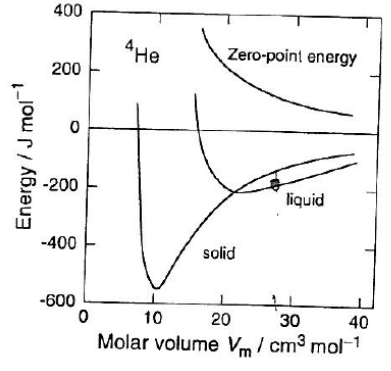
\includegraphics[width=0.9\linewidth]{Immagini - Capitolo 1/He U(T) senza E0.png}
        \caption{energia potenziale $U$ in funzione di $T$ dell'elio-4 senza $E_0$.}
        \label{fig: He U(T) senza E0}
    \end{subfigure}
    \hspace{0.1pt}
    \begin{subfigure}[t]{0.4\linewidth}
        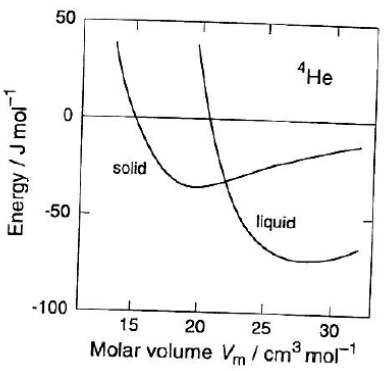
\includegraphics[width=0.9\linewidth]{Immagini - Capitolo 1/He U(T) con E0.png}
        \caption{energia potenziale $U$ in funzione di $T$ dell'elio-4 con $E_0$.}
        \label{fig: He U(T) con E0}
    \end{subfigure}
\end{figure}

Si consideri una particella racchiusa in una buca di potenziale infinita di lunghezza $L$, le energie accessibili al sistema sono
\begin{equation}
    E_n = \frac{\hbar^2\pi^2}{2mL^2}\sum_{i=1}^3(n_i+1)^2,
\end{equation}
quindi l'energia di punto zero è 
\begin{equation}
    E_0 = \frac{3\hbar^2\pi^2}{2mV^{2/3}} \simeq \frac{1}{V^{2/3}}.
\end{equation}
Quindi, a $T = \SI{0}{\kelvin}$ a pressione atmosferica è la fase liquida ad essere più stabile con un volume molare di circa $\SI{28}{\centi\meter\cubed\mol^{-1}}$, come mostrato in figura \ref{fig: He U(T) con E0}. In tabella \ref{tab: parametri del 3He e 4He} sono riportati alcuni parametri caratteristici dell'elio-3 e dell'elio-4.
\begin{table}[h]
    \centering
    \begin{tabular}{|c|cc|}
         \hline 
         & $\ce{^3He}$ & $\ce{^4He}$ \\ \hline
         temperatura di ebollizione a $\SI{1}{\atm}$ $[\mathrm{K}]$ & 3.19 & 4.21 \\
         temperatura critica $[\mathrm{K}]$ & 3.32 & 5.19 \\
         pressione critica $[\mathrm{bar}]$ & 1.16 & 2.29 \\
         densità per $T \to 0$ $[\SI{}{\gram\per\centi\meter\cubed}]$ & 0.076 & 0.145 \\
         densità al punto di ebollizione $[\SI{}{\gram\per\centi\meter\cubed}]$ & 0.055 & 0.125 \\ \hline
    \end{tabular}
    \caption{alcuni importanti parametri dell'elio-3 e dell'elio-4.}
    \label{tab: parametri del 3He e 4He}
\end{table}

Onnes scopre che la densità dell'$\ce{^4He}$ è eccezionalmente bassa e osserva che presenta un massimo intorno alla temperatura di $\SI{2}{\kelvin}$, come mostrato nel grafico in figura \ref{fig: He rho(T)}.
\begin{figure}[h]
    \centering
    \begin{subfigure}[t]{0.4\linewidth}
        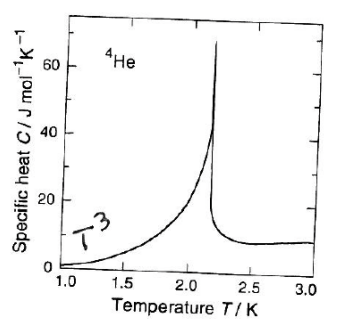
\includegraphics[width=0.9\linewidth]{Immagini - Capitolo 1/He c(T).png}
        \caption{andamento del calore specifico $c$ dell'elio-4 in funzione di $T$.}
        \label{fig: He c(T)}
    \end{subfigure}
    \begin{subfigure}[t]{0.4\linewidth}
        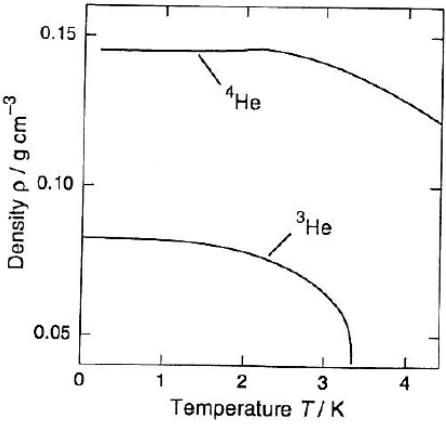
\includegraphics[width=0.9\linewidth]{Immagini - Capitolo 1/He rho(T).png}
        \caption{diagramma $p(T)$ dell'elio-4.}
        \label{fig: He rho(T)}
    \end{subfigure}
\end{figure}
Nel 1923 Dana ed Onnes osservano sperimentalmente che il calore specifico dell'elio-4 cresce vertiginosamente sempre intorno ai $\SI{2}{\kelvin}$, sempre mostrato in figura \ref{fig: He c(T)}, ma il fatto fu inizialmente attribuito ad un problema sperimentale dovuto alle difficoltà tecniche dell'esperimento. Tuttavia, nel 1932 con il miglioramento della tecnologia, Keesam e Clausius confermarono la validità della scoperta di Onnes e Dana alla temperatura $T_\Lambda = \SI{2.17}{\kelvin}$. Poiché la natura della transizione rimaneva sconosciuta, per molto tempo le due fasi dell'elio vennero battezzate con i nomi di elio-I per $T > T_\Lambda$ e elio-II per $T < T_\Lambda$. Il motivo per cui la temperatura di transizione è indicata con $T_\Lambda$ è che l'andamento della curva del calore specifico in funzione di $T$ ricorda la forma della lettera greca in questione. Il punto di transizione venne infatti denominato ``$\Lambda$-point''. 
\begin{obs}
    Inizialmente, si pensava che l'elio-II fosse una fase ``solida'' del tipo cristallo liquido.
\end{obs}
Al contrario di ciò che si pensava inizialmente il calore specifico non tende ad infinito, invece è approssimabile con una funzione a tratti
\begin{equation}
    c_V = 
    \begin{cases}
        c(T) + A_+|T - T_\Lambda|^{-\alpha},\quad T > T_\Lambda \\
        c(T) + A_-|T - T_\Lambda|^{-\alpha},\quad T < T_\Lambda
    \end{cases},\quad \alpha = 0.009,
\end{equation}
dove $c(T)$ è una funzione continua. La transizione quindi è del secondo ordine in quanto 
\begin{equation}
    S = -\frac{\p G}{\p T}\bigg|_p,\quad c_V = -T\frac{\p^2G}{\p T^2}\bigg|_p
\end{equation}
sono funzioni continue. Sempre Dana ed Onnes osservarono che il calore latente di vaporizzazione $L$ ha un minimo intorno ai $\SI{0.8}{\kelvin}$ e tende a crescere per temperature ancora minori. Il diagramma delle fasi $p(T)$ dell'elio-4 è riportato in figura \ref{fig: He p(T)}. Partendo dall'energia libera di Gibbs si ha che all'equilibrio le energie della fase solida e liquida si equivalgono, per cui 
\begin{equation}
\label{eq: equilibrio fase liquida e solida elio-4}
    G_{l} \simeq G_s\quad\Longrightarrow\quad \mu_l \simeq \mu_s.
\end{equation}
\begin{figure}[h]
    \centering
    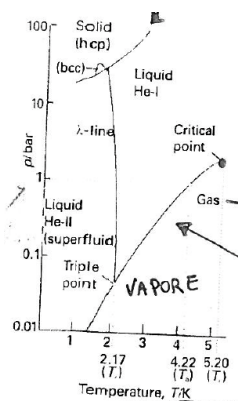
\includegraphics[width=0.25\linewidth]{Immagini - Capitolo 1/He p(T).png}
    \caption{grafico $p(T)$ dell'elio-4.}
    \label{fig: He p(T)}
\end{figure}

Adesso conoscendo le equazioni di stato $\p_TG = - S$ e $\p_pG = V$ si può espandere l'espressione \eqref{eq: equilibrio fase liquida e solida elio-4} ottenendo
\begin{align}
    \frac{\p G_l}{\p T}\delta T + \frac{\p G_l}{\p p}\delta p &= \frac{\p G_s}{\p T}\delta T + \frac{\p G_s}{\p p}\delta p \\
    V_l\delta p - S_l \delta T &= V_s\delta T - S_s\delta p,
\end{align}
da cui, riarrangiando i termini, si trova l'equazione di Clausius-Clapeyron
\begin{equation}
\label{eq: equazione di Clausius-Clapeyron}
    \frac{dp}{dT} = \frac{S_s - S_l}{V_s - V_l} = \frac{\Delta S}{\Delta V}.
\end{equation}
Dato che $V_l > V_s$ se $dp/dT < 0$ per $T < \SI{0.8}{\kelvin}$, allora $S_s > S_l$. Quindi, l'entropia del solido di $\ce{^4He}$ è maggiore di quella della fase liquida. 

Una delle caratteristiche più importanti dell'elio-II è la proprietà di passare attraverso capillari senza essere oggetto della forza d'attrito. Questa proprietà di superfluidità venne scoperta da Kapitza, e indipendentemente da Allen e Misener. Per spiegare la natura di questa proprietà, nel 1938 London suggerisce sia legata alla condensazione di Bose-Einstein. Adottando questo punto di vista, Tisza formula un modello fenomenologico ``a due fluidi''. Quando la temperatura tende a zero, la lunghezza d'onda di de Broglie $\lambda$ diventa paragonabile alla distanza interatomica e gli atomi perdono la loro identità comportandosi come onde. 
\begin{figure}[h]
    \centering
    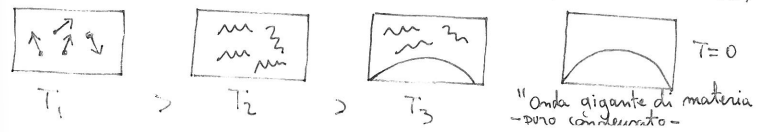
\includegraphics[width=0.9\linewidth]{Immagini - Capitolo 1/comportamento ondulatorio atomi.png}
    \caption{evoluzione verso un comportamento ondulatorio degli atomi del condensato.}
    \label{fig: comportamento ondulatorio atomi}
\end{figure}

Infatti, se la lunghezza d'onda di de Broglie è  $\lambda = h/p$, con il fatto che $p=mv$ e tramite il teorema di equipartizione dell'energia che restituisce la relazione 
\begin{equation}
    \frac{1}{2}m\vmedio{v^2} = \frac{3}{2}kT
\end{equation}
si può definire la lunghezza di de Broglie termica come
\begin{equation}
    \lambda_T = \frac{h}{\sqrt{3mkT}}.
\end{equation}
Per $T = \SI{300}{\kelvin}$ si ha che $\lambda_T = \SI{e-8}{\centi\meter}$, mentre per $T = \SI{e-8}{\kelvin}$ si trova $\lambda_T = \SI{e-3}{\centi\meter}$. A temperature $T > T_\Lambda$ l'elio liquido si comporta come un gas molto denso, ma a $T = T_\Lambda$ quasi tutte le proprietà dell'elio cambiano drasticamente. Seguendo la linea di ebollizione si ha che l'elio si comporta come come un fluido normale, ossia che è soggetto ad ebollizione, mentre a temperature minori di $T_\Lambda$ questo smette di bollire. Questo è dovuto al fatto che la capacità termica diventa cinque ordini di grandezza più grande di quella dell'elio-I. Dunque, in generale non è possibile impostare un gradiente di temperatura in un superfluido, come non è possibile impostare una differenza di potenziale ai capi di un conduttore ideale con resistenza nulla. Inoltre, l'elio per $T < T_\Lambda$ non ha viscosità. Esiste anche un altro effetto detto ``meccano-calorico''. Dati due recipienti contenenti elio alla stessa temperatura e pressione collegati da un capillare molto sottile a $T < T_\Lambda$, come mostrato in figura \ref{fig: esperimento capillare}, se si incrementa la pressione $p_A$, allora il livello in $A$ si abbassa e quello in $B$ si alza, come ci si aspetta per un fluido incomprimibile.
\begin{figure}[h]
    \centering
    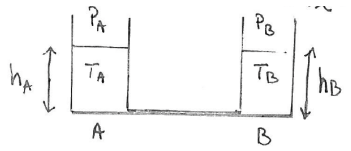
\includegraphics[width=0.5\linewidth]{Immagini - Capitolo 1/esperimento capillare.png}
    \caption{esperimento del capillare.}
    \label{fig: esperimento capillare}
\end{figure}
Tuttavia, corrispondentemente la temperatura in $B$ si abbassa, mentre quella in $A$ aumenta, pertanto attraverso il capillare passa solamente la componente superfluida a $S = 0$. Esiste anche l'effetto inverso detto ``termomeccanico''. Nella medesima situazione, se si aumenta la temperatura di $A$ si osserva una differenza di livello nei due recipienti, in particolare $h_A > h_B$. Nell'esperimento del beaker si osserva come l'elio supefluido possieda una tensione superficiale non nulla; infatti, l'elio in questa fase riesce ad arrampicarsi fuori dalle pareti di un contenitore per ottenere l'equilibrio chimico pur avendo viscosità nulla. Inoltre, nell'elio-II si osservano delle onde di temperatura che si propagano ad una velocità caratteristica, ciò è dovuto all'enorme capacità termica. Poiché la propagazione avviene in modo molto simile a quanto si osserva con le onde sonore, questo effetto è stato rinominato come ``secondo suono''. Tutte queste proprietà derivano dal ``modello a due fluidi'' di Tisza.

\section{Modello a due fluidi}
L'idea è di considerare l'elio-II come composto da un insieme di due fluidi completamente interpenetranti con proprietà diverse. Anche se questa interpretazione non è totalmente corretta\footnote{Infatti, non è possibile che nell'elio-II vi siano atomi appartenenti ad un fluido normale ed altri appartenenti ad un superfluido: gli atomi sono indistinguibili e la funzione d'onda totale deve essere simmetrica per lo scambio di particelle.}, il modello gode di un discreto successo. Si supponga quindi che la densità dell'elio-II si possa separare in due contributi dovuti al fluido normale e al superfluido rispettivamente, in tal caso
\begin{equation}
    \rho_{\ce{^4He}} = \rho_N(T) + \rho_S(T),
\end{equation}
dove i due termini dipendono dalla temperatura $T$. A $T = \SI{0}{\kelvin}$ l'elio-II è composto unicamente dal superfluido e $\rho_N = 0$, invece per $T \ge T_\Lambda$ è presente solo la componente ordinaria e $\rho_S  = 0$.
\begin{figure}[h]
    \centering
    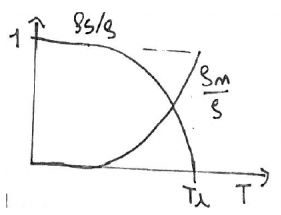
\includegraphics[width=0.3\linewidth]{Immagini - Capitolo 1/He rhoS(T).png}
    \caption{andamento di $\rho_S/\rho$ in funzione di $T$.}
    \label{fig: He rhoS(T)}
\end{figure}
La densità $\rho$ dipende anche dalla temperatura, ma le fluttuazioni nel range che si sta considerando sono minime. Nel caso dei bosoni liberi si ha che $\rho_S = \rho_0 = 0$, mentre nel caso dell'elio la situazione è complicata a causa dell'interazione intermolecolare; infatti, gli atomi perdono la loro identità e sono le eccitazioni collettive che diventano importanti. Anche a $T = \SI{0}{\kelvin}$ si ha $\rho_N \neq \rho_S$, per cui non tutte le particelle rimangono nello stato con $\vk = 0$, portando al fenomeno della deplezione quantistica. Conviene quindi identificare $\rho_N$ con la densità di eccitazioni collettive. Si noti che il calore specifico $c_V$ nell'elio-II a $T \simeq \SI{0}{\kelvin}$ cresce come $T^3$ e il sistema si comporta come un gas di fononi non interagenti.
\begin{table}[h]
    \centering
    \begin{tabular}{|c|ccc|}
         \hline
         componente & densità & viscosità & entropia \\ \hline
         normale & $\rho_N$ & $\eta_N \neq 0$ & $S_N \neq 0$ \\
         superfluida & $\rho_S$ & $\eta_S = 0$ & $S_S = 0$ \\ \hline
    \end{tabular}
    \caption{caratteristiche delle componenti normale e superfluida dell'$\ce{^4He}$.}
    \label{tab: caratteristiche componenti 4He}
\end{table}

\subsection{Effetto termomeccanico}
L'effetto termomeccanico è una conseguenza dell'equazione \eqref{eq: equazione di Clausius-Clapeyron} ottenuta imponendo $d\mu = 0$ all'equilibrio. Si supponga di avere due contenitori $A$ e $B$ con $\ce{^4He}$ a $T < T_\Lambda$. I contenitori sono completamente isolati, ossia adiabatici e rigidi, ma collegati tra loro da un capillare che fa passare solo la componente superfluida. Se non avvengono processi irreversibili, l'entropia totale $S$ del sistema $A + B$ è costante, come mostrato in figura \ref{fig: effetto termomeccanico}.
\begin{figure}[h]
    \centering
    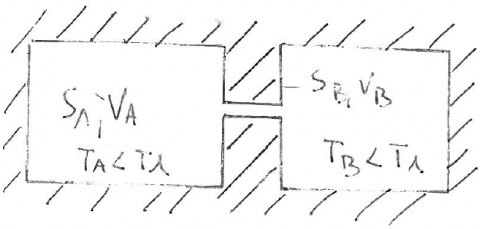
\includegraphics[width=0.4\linewidth]{Immagini - Capitolo 1/effetto termomeccanico.png}
    \caption{sistema isolato contenente elio-4 a $T < T_\Lambda$.}
    \label{fig: effetto termomeccanico}
\end{figure}
Poiché attraverso il capillare può solo passare la componente superfluida con $S = 0$, allora anche l'entropia all'interno dei due contenitori è costante, per cui $S_A$ e $S_B$ sono costanti. Si denota con $U_T$ l'energia interna totale e con $U_l$, dove $l = \{A,B\}$, l'energia interna per unità di massa definita come 
\begin{equation}
    U_T = \sum_{l=A,B}M_lu_l,
\end{equation}
dove $M_l$ è la massa di $\ce{^4He}$ nel rispettivo contenitore. All'equilibrio termodinamico l'energia interna totale è minima, quindi 
\begin{equation}
    \delta U_T = \sum_{l=A,B}(u_l\delta M_l + M_l\delta u_l) = 0.
\end{equation}
Poiché anche l'entropia $S_l$ è costante, quindi 
\begin{equation}
\label{eq: variazione entropia s_l}
    \delta S_l = s_l\delta M_l + M_l\delta s_l = 0 \quad\Longrightarrow\quad \delta s_l = -s_l\frac{\delta M_l}{M_l}.
\end{equation}
Il volume $V_l = M_lv_l$ è anche costante, per cui
\begin{equation}
\label{eq: variazione volume v_l}
    \delta v_l = -v_l\frac{\delta M_l}{M_l}.
\end{equation}
Sviluppando ora $\delta u_l(s,v)$ si trova
\begin{equation}
    \delta u_l = \frac{\p u}{\p s_l}\bigg|_{v_l}\delta s_l + \frac{\p u}{\p v_l}\bigg|_{s_l}\delta v_l,
\end{equation}
con il quale ponendo si ricava
\begin{equation}
    \delta U_T = \nsum_l\bigg[u_l\delta M_l + M_l\bigg(\frac{\p u}{\p s_l}\bigg|_{v_l}\delta s_l + \frac{\p u}{\p v_l}\bigg|_{s_l}\delta v_l\bigg)\bigg] = 0,
\end{equation}
ma sapendo che 
\begin{equation}
    \frac{\p u}{\p s}\bigg|_v = T,\quad \frac{\p u}{\p v}\bigg|_s = -p,
\end{equation}
si arriva a 
\begin{equation}
    \nsum_l[u_l\delta M_l + M_l(T_l\delta s_l - p_l\delta v_l)] = 0
\end{equation}
dove sostituendo le relazioni \eqref{eq: variazione entropia s_l} e \eqref{eq: variazione volume v_l} si trova
\begin{equation}
    \nsum_l(u_l - s_lT_l + v_lp_l)\delta M_l = \nsum_l \mu_l \delta M_l = 0,
\end{equation}
ma se la massa è conservata $\delta M_A = - \delta M_B$ e quindi si trova la condizione di equilibrio chimico
\begin{equation}
    \mu_A(T_A,p_A) = \mu_B(T_B,p_B).
\end{equation}
Anche per $T_A \neq T_B$ si raggiunge l'equilibrio $\mu_A = \mu_B$ attraverso lo scambio di atomi ad entropia nulla, modificando quindi anche $p_A$ e $p_B$. Se $T_A = T_B + \delta T$ e $p_A = p_B + \delta p$, allora sviluppando al primo ordine $\mu_A$ si ottiene
\begin{equation}
    \frac{\p\mu_A}{\p T_A}\delta T + \frac{\p \mu_A}{\p p_A}\delta p = 0,
\end{equation}
da cui si ricava l'equazione di London 
\begin{equation}
\label{eq: equazione di London}
    \delta p = \frac{s_A}{v_A}\delta T.
\end{equation}
Dunque, se aumenta la differenza di temperatura, aumenta proporzionalmente la differenza di pressione a causa di un flusso di atomi della componente superfluida che attraversa il capillare dal contenitore $B$ ad $A$. L'effetto termomeccanico si può osservare anche nell'esperimento della fontanella. Come mostrato in figura \ref{fig: esperimento fontanella}, l'elio è riscaldato nella zona del gomito da un fascio molto tenue di luce. Dell'elio superfluido entra nel tubo attraverso il filtro capillare per mantenere il potenziale chimico, ma questo fa aumentare il livello dell'elio nel tubo verticale che fuoriesce dall'apertura superiore creando una fontanella. Attraverso il filtro capillare si instaura quindi un flusso spontaneo dal contenitore ``freddo'' all'interno del tubo ``caldo''. Poiché il superfluido dal contenitore non trasporta entropia, questo processo non viola il secondo principio della Termodinamica. Fontanelle stazionarie di circa $\SI{30}{\centi\meter}$ sono state ottenute in questo modo. Di solito il flusso è turbolento, ma in certe condizioni le fontanelle possono esserne prive. 
\begin{figure}[h]
    \centering
    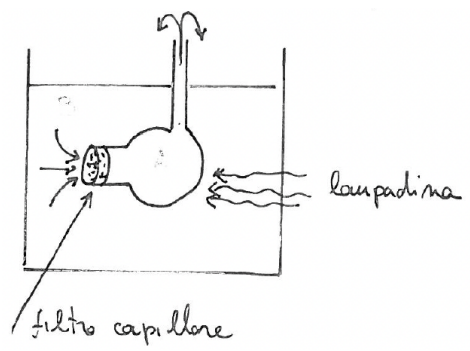
\includegraphics[width=0.4\linewidth]{Immagini - Capitolo 1/esperimento fontanella.png}
    \caption{esperimento della fontanella.}
    \label{fig: esperimento fontanella}
\end{figure}

La spiegazione del comportamento stranormale dell'elio liquido nell'esperimento del beaker può essere spiegato utilizzando i potenziali chimici. Considerando il diagramma in figura \ref{fig: esperimento beaker}, l'elio forma una pellicola sottile sulla superficie del recipiente sopra il livello dell'elio liquido. La pellicola si forma a causa dell'interazione di van der Waals tra gli atomi di elio e le pareti del contenitore. All'equilibrio si ha 
\begin{equation}
\label{eq: condizione equilibrio esperimento beaker}
    \mu_{film}(z) = \mu_{vap} = \mu_l(z = 0) \equiv \mu_l(0).
\end{equation}
Poiché si sono forze esterne come quella di van der Waals e la gravità, questi sono i potenziali chimici totali, con $\mu_{film}$ corrispondente alla somma di tre termini
\begin{equation}
    \mu_{film}(z) = \mu_l(0) + \mu_g(z) + \mu_{vdW}(z) = \mu_l(0) \Longrightarrow \mu_g = gz = - \mu_{vdW},
\end{equation}
dove si è usata la \eqref{eq: condizione equilibrio esperimento beaker}. 
\begin{figure}[h]
    \centering
    \begin{subfigure}[t]{0.4\linewidth}
        \centering
        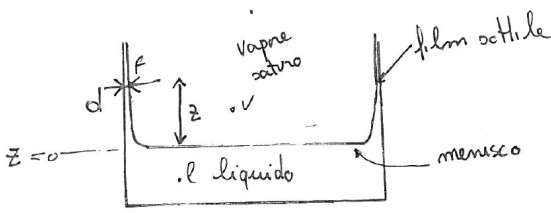
\includegraphics[width=0.95\linewidth]{Immagini - Capitolo 1/esperimento beaker.png}
        \caption{esperimento del beaker.}
        \label{fig: esperimento beaker}
    \end{subfigure}
    \begin{subfigure}[t]{0.4\linewidth}
        \centering
        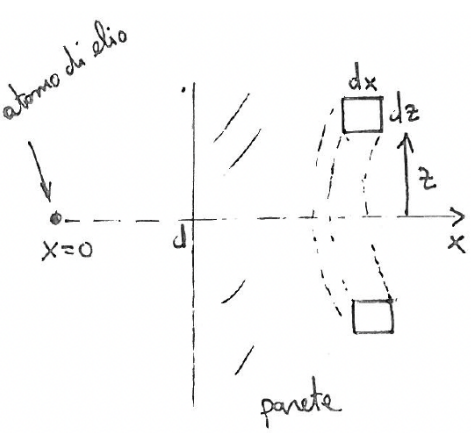
\includegraphics[width=0.7\linewidth]{Immagini - Capitolo 1/esperimento beaker (calcolo).png}
        \caption{costruzione per l'esperimento del beaker.}
        \label{fig: esperimento beaker (calcolo)}
    \end{subfigure}
\end{figure}

Il potenziale chimico di van der Waals si ottiene integrando il potenziale $\phi(r) \propto -1/r^6$. Lo spessore della parete è dell'ordine del millimetro, quindi molto più grande delle distanze interatomiche, per cui è approssimabile ad uno spessore infinito. Si divide quindi lo spazio nella parete di destra in corone circolari con sezione $dx$ per $dz$ e raggio $z$, come mostrato in figura \ref{fig: esperimento beaker (calcolo)}. Quindi, 
\begin{equation}
    \begin{split}
        \mu_{vdW} \propto -\int_d^\infty dx\int _0^\infty dz\, \frac{2\pi z}{(z^2 + x^2)^3} &\overset{y=z^2}{=} -\int_d^\infty dx \int _0^\infty dy\,\frac{\pi}{(x^2 + y^2)^3} \\
        &= -\int_d^\infty dx\,\bigg[\frac{-\pi}{2}(x^2 + y^2)^{-2}\bigg]_0^\infty \\
        &= -\frac{\pi}{2}\int_d^\infty \frac{dx}{x^4} \\
        &= -\frac{\pi}{6d^3}.
    \end{split}
\end{equation}
Dunque, $\mu_{vdW} = -\alpha/d^3$ dove $\alpha$ è la costante di Hamaker. In totale da $\mu_g = gz = -\alpha/d^3$ si ha l'equazione del menisco
\begin{equation}
\label{eq: equazione del menisco}
    d = \sqrt[3]{\frac{\alpha}{gz}}.
\end{equation}
La costante $\alpha$ è ottenuta a partire dalle proprietà dielettriche dell'elio e dalle pareti del recipiente misurate sperimentalmente. All'equilibrio in condizione di vapore saturo si trova che a $z = \SI{10}{\centi\meter}$ lo spessore del film è $d \simeq \SI{200}{\angstrom}$. Un fluido normale non potrebbe scorrere in un capillare di queste dimensioni. Le proprietà superfluida dell'elio non sono importanti per determinare lo spessore del film ma lo sono per perché scorrere all'interno del film senza attrito. L'elio superfluido si diffonde su tutte le pareti per minimizzare il potenziale chimico ovunque. 

\subsection{Secondo suono}
Le variazioni di temperatura in un sistema omogeneo si propagano nel mezzo in accordo con l'equazione di propagazione del calore
\begin{equation}
\label{eq: equazione di propagazione del calore}
    \nabla^2 T = \frac{1}{D}\frac{\p }{\p t}T(\vx,t).
\end{equation}
Nell'elio-II la conducibilità termica $D$ è infinita, quindi l'equazione precedente non è più valida. Si può pensare che il membro di destra dell'equazione \eqref{eq: equazione di propagazione del calore} sia in realtà il primo termine di uno sviluppo in serie di Taylor in $t$: se il primo termine è zero, il termine successivo con la derivata seconda non è più trascurabile; perciò ci si aspetta che l'equazione venga modificata nel modo seguente
\begin{equation}
    \nabla^2 T = \frac{1}{v}\frac{\p^2 T}{\p t^2},
\end{equation}
che rappresenta la propagazione per onde delle variazioni di temperatura. Dunque. nell'elio-II ci si aspettano due tipi di propagazione per onde:
\begin{enumerate}
    \item il suono, ossia la propagazione di onde di pressione o densità descritte dall'equazione di d'Alembert $\square\rho = 0$, dove $\rho_N$ e $\rho_S$ sono indistinguibili e oscillano in fase;
    \item il secondo suono, ossia la propagazione di onde termiche, legate a fluttuazioni di $\rho_N$ a $\rho$ costante, dove $\rho_N$ e $\rho_S$ oscillano in opposizione di fase.
\end{enumerate}
Una variazione locale di $\rho_N$ corrisponde ad una variazione locale della temperatura, quindi il secondo suono è un'onda di temperatura. Nell'ambito del modello a due fluidi è facile derivare l'equazione di propagazione del secondo suono nel caso del gas di fononi (elio-II a $T \simeq \SI{0}{\kelvin}$). Si indica con $u = U/V$ l'energia per unità di volume del gas di fononi. L'equazione della meccanica $\vF = m\va$ per un fluido si traduce in 
\begin{equation}
    \frac{d\vq}{dt} = -\nabla p,
\end{equation}
dove $\vq$ è la quantità di moto per unità di volume. D'altra parte, l'equazione di continuità per l'energia è
\begin{equation}
    \frac{1}{v_1^2}\frac{d u}{dt} + \nabla \cdot \vq = 0,
\end{equation}
da cui si ha
\begin{equation}
    \frac{\p ^2u}{\p t^2} = v_1^2\nabla^2 p.
\end{equation}
Tuttavia, per un gas di fononi la pressione $p$ è legata alla densità di energia da 
\begin{equation}
    p = - \frac{\p F(T,V)}{\p V}\bigg|_T,\quad F(T,V,N) = U(S,V,N) - \frac{\p U}{\p S}S,
\end{equation}
quindi sapendo anche che
\begin{equation}
    F = -\frac{U}{3} = -\frac{\sigma VT^4}{3},
\end{equation}
dove $\sigma$ nel caso del corpo nero sarebbe la costante di Stefan-Boltzmann, si ha
\begin{equation}
    p = \frac{\sigma T^4}{3} = \frac{u}{3}.
\end{equation}
Quindi, si ottiene
\begin{equation}
    \frac{\p ^2 u}{\p t^2} - \frac{v_1^2}{3}\nabla^2 u = 0
\end{equation}
e dunque la velocità del secondo suono è 
\begin{equation}
    v_2 = \frac{v_1}{\sqrt{3}}.
\end{equation}
Le fluttuazioni della densità dei fononi si propagano con una velocità caratteristica pari a $v_2 \simeq \SI{137}{\meter\per\second}$ a $T = \SI{0}{\kelvin}$, ma per problemi tecnici, questo valore limite per $T < \SI{0.5}{\kelvin}$ non è ancora stato confermato dagli esperimenti. Le fluttuazioni in $u$ sono legate a quelle in $T$ dal fatto che $\delta u \propto \bar{T}^3\delta T$.
\begin{figure}[h]
    \centering
    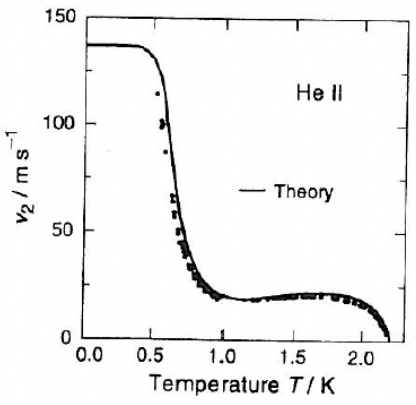
\includegraphics[width=0.35\linewidth]{Immagini - Capitolo 1/He v2(T).png}
    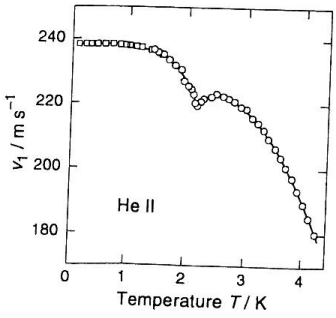
\includegraphics[width=0.35\linewidth]{Immagini - Capitolo 1/He v1(T).png}
    \caption{andamento in funzione di $T$ del: (i) primo suono $v_1$; (ii) secondo suono $v_2$.}
    \label{fig: He v1(T) e v2(T)}
\end{figure}

\subsection{Velocità critica}
Dopo aver discusso il fenomeno del secondo tramite la verifica della propagazione di onde di temperatura ad una velocità caratteristica, si passa ad analizzare una proprietà fondamentale dei superfluidi: avere viscosità nulla. La viscosità è la manifestazione macroscopica dello scambio di energia tra un fluido in scorrimento e la parte lungo cui scorre. Poiché questo scambio avviene per quanti, dove le eccitazioni sono quasi-particelle, può succedere che per ragioni cinematiche un fluido a $T = \SI{0}{\kelvin}$ che scorre a velocità inferiore ad un valore critico non possa produrre quasi-particelle nell'interazione con la parete, non perdendo quindi energia ed avendo allora viscosità nulla. Il tutto dipende dalla relazione di dispersione che lega l'energia $\epsilon$ all'impulso $\vq$ delle quasi-particelle. Nell'elio superfluido, la diffusione inelastica con fasci di neutroni permette di stabilire che la curva di dispersione ha approssimativamente la forma mostrata in figura \ref{fig: He e(q)}. Per piccoli valori di $q$, ossia per grandi lunghezze d'onda, si ha $\epsilon(q) = v_1 q$, dove $v_1$ è la velocità del primo suono a $T = \SI{0}{\kelvin}$. Eccitazioni di questo tipo sono i quanti del suono, cioè i fononi. Queste sono le eccitazioni più importanti per il comportamento termico del fluido a $T < \SI{0.5}{\kelvin}$. Al di sopra di questa temperatura entra in gioco un altro tipo di quasi-particella, il rotone, corrispondete al minimo locale nella curva di dispersione. Si cercano ora i vincoli cinematici per la produzione di una particella con impulso $\vq$ ed energia $\epsilon(q)$ da parte di un fluido di massa $M$ che scorre lungo una parete con velocità $\vv$. Per la conservazione dell'impulso e per la conservazione dell'energia si hanno
\begin{equation}
    \begin{cases}
        M\vv = M\vv' + \vq \\[1.5ex]
        \dfrac{1}{2}Mv^2 = \dfrac{1}{2}M(v')^2 + \epsilon(q)
    \end{cases}
\end{equation}
da cui, sostituendo $\vv' = \vv - \vq/M$ nella seconda equazione, si trova
\begin{equation}
    \vv \cdot \vq - \frac{q^2}{2M} = \epsilon(q).
\end{equation}
Considerando il limite in cui $M \to \infty$, si ottiene che
\begin{equation}
   \vv \cdot \vq = \epsilon(q)\quad\Longrightarrow\quad v > \frac{\epsilon(q)}{q},
\end{equation}
per cui esiste una velocità critica $v_c$ sotto la quale il fluido ha viscosità nulla data dalla velocità di London 
\begin{equation}
    v_c = \min_{q}\bigg\{\frac{\epsilon(q)}{q}\bigg\}.
\end{equation}
In conclusione, ogni sostanza che è liquida a $T = \SI{0}{\kelvin}$ ed ha uno spettro di eccitazioni formato, a bassa energia, da fononi è necessariamente un superfluido a tale temperatura perché esiste una velocità critica $v_c > 0$.
\begin{figure}[h]
    \centering
    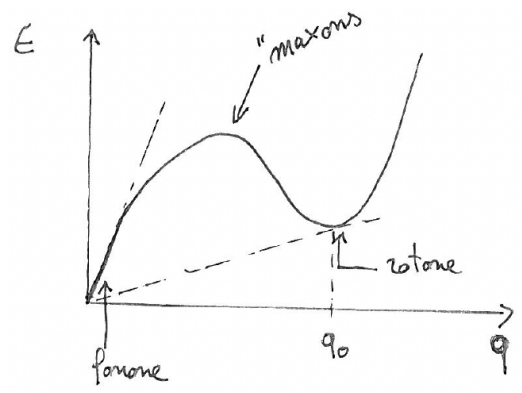
\includegraphics[width=0.35\linewidth]{Immagini - Capitolo 1/He e(q).png}
    \caption{andamento di $\epsilon$ in funzione di $q$ dell'elio superfluido.}
    \label{fig: He e(q)}
\end{figure}
\begin{obs}
    Per lungo tempo si pensò che la superfluidità fosse legata all'esistenza di un gap di energia, in analogia al fenomeno della superconduttività; tuttavia, ciò non è possibile a causa del fatto che i fononi possono avere un'energia arbitrariamente piccola.
\end{obs}
Per $T > \SI{0}{\kelvin}$ il ragionamento precedente continua a valere, ma adesso il liquido contiene un gas di fononi, o più in generale di quasi-particelle, che possono interagire con le pareti dando luogo ad un comportamento viscoso. Le velocità critiche sono 
\begin{equation}
    v_c(fononi) \simeq \SI{238}{\meter\per\second} \equiv v_1,\quad v_c(rotoni) \simeq \SI{60}{\meter\per\second} \equiv \frac{\epsilon(q_0)}{q_0}.
\end{equation}
Lo stesso Landau pensava che la velocità critica osservata negli esperimenti fosse determinata dai rotoni, tuttavia risulta invece che a pressione ambiente si possono creare vortici ad anello a velocità considerevolmente inferiore a quella critica dei rotoni. Nel gas di bosoni ideale si ha che l'energia è pari all'energia cinetica $\epsilon(q) = q^2/2m$, per cui la velocità critica è
\begin{equation}
    v_c = \min_q{\bigg(\frac{\epsilon(q)}{q}\bigg)} = \min_q{\bigg(\frac{q}{2m}\bigg)} = 0.
\end{equation}
Dunque, il gas di bosoni ideale non è un superfluido. L'interpretazione microscopica dei fononi e dei rotoni è molto diversa. A piccoli valori di $q$, un atomo di elio è fortemente accoppiato agli altri atomi del condensato e i fononi corrispondono alle tipiche onde di compressione e rarefazione nei fluidi e nei solidi. Per valori di $q$ molto grandi, le particelle si muovono quasi liberamente nel condensato e la curva di dispersione cresce come
\begin{equation}
    \epsilon(q) \simeq \frac{q^2}{2m^*} + \mu,\quad q \gg 0,
\end{equation}
dove $m^*$ è la massa efficace. Per valori intermedi dell'impulso, un atomo in movimento è fortemente accoppiato solo con i minimi vicini. Quando avanza, quelli che lo precedono si spostano lateralmente per poi passargli dietro; l'effetto netto è simile a quello di un anello vorticoso, come mostrato in figura \ref{fig: fononi e rotoni}. 
\begin{figure}[h]
    \centering
    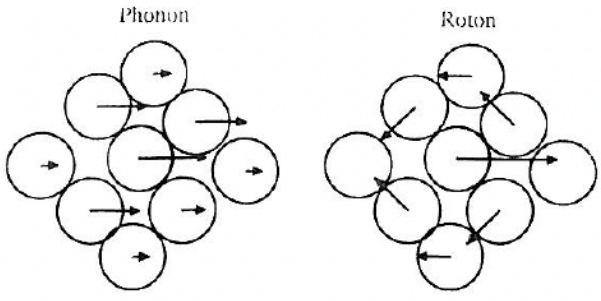
\includegraphics[width=0.4\linewidth]{Immagini - Capitolo 1/fononi e rotoni.png}
    \caption{comportamento dei fononi e dei rotoni.}
    \label{fig: fononi e rotoni}
\end{figure}

\section{Stato quantistico macroscopico}
L'equazione di Schr\"odinger che descrive un sistema di $N$ bosoni identici è
\begin{equation}
\label{eq: equazione di Schrodinger per un gas di bosoni}
    i\hbar\frac{\p}{\p t}\phi(\vr_1,\dots,\vr_N;t) = \hatH_N\phi(\vr_1,\dots,\vr_N;t),
\end{equation}
con hamiltoniana
\begin{equation}
\label{eq: hamiltoniana per un gas di bosoni}
    \hatH_N = \sum_{i=1}^N\bigg[-\frac{\hbar^2}{2m}\nabla^2 + V_{ext}(\vr_i)\bigg] + \frac{1}{2}\sum_{i\neq j}V(|\vr_i - \vr_j|),
\end{equation}
dove $\{\vr_i\}$ è l'insieme delle coordinate delle particelle, $V(|\vr_i - \vr_j|)$ è il potenziale interatomico e $V_{ext}(\vr_i)$ è il potenziale esterno. Dato che le particelle sono bosoni, la funzione d'onda deve essere simmetrica per lo scambio di particelle
\begin{equation}
\label{eq: simmetria per permutazioni della funzione d'onda di un gas di bosoni}
    \phi(\vr_1,\dots,\vr_i,\vr_j,\dots,\vr_N;t) = \phi(\vr_1,\dots,\vr_j,\vr_i,\dots,\vr_N;t).
\end{equation}
Nel caso in cui tutte le particelle siano nello stato fondamentale quantistico, per cui $N \to N_0$ a $T = \SI{0}{\kelvin}$, si può introdurre l'approssimazione di Hartree-Fock per cui la funzione d'onda si fattorizza secondo
\begin{equation}
\label{eq: approssimazione di Hartree-Fock per un gas di bosoni}
    \phi_0(\vr_1,\dots,\vr_{N_0}) = \prod_{i=1}^{N_0} \frac{\phi_0(\vr_i)}{\sqrt{N_0}},
\end{equation}
dove la funzione d'onda di singola particella è normalizzata con
\begin{equation}
\label{eq: normalizzazione funzione d'onda in approssimazione di Hartree-Fock}
    \int d^3r\,\phi_0^*(\vr)\phi_0(\vr) = \int d^3r\,\frac{\rho_S(\vr)}{m} = \int d^3r\,n_S(\vr) = N_0.
\end{equation}
Nell'approssimazione di Hartree-Fock lo stato quantistico macroscopico presente nell'elio-II e nel condensato di Bose-Einstein a $T = \SI{0}{\kelvin}$ può essere descritto dalla funzione d'onda
\begin{equation}
    \phi_0(\vr) = |\phi_0(\vr)|e^{i\theta(\vr)} = \sqrt{n_S(\vr)}e^{i\theta(\vr)}.
\end{equation}
La fase della funzione d'onda è legata alla velocità del superfluido; infatti, si può introdurre la densità di corrente
\begin{equation}
    \vj_S(\vr) = -\frac{i\hbar}{2m}(\phi_0^*\nabla\phi_0 - \phi_0\nabla\phi_0^*) = n_S(\vr)\frac{\hbar}{m}\nabla\theta(\vr) \equiv n_S(\vr)\vv_S(\vr).
\end{equation}
Quindi, si può determinare che la relazione tra la velocità e la fase è
\begin{equation}
    \vv_S = \frac{\hbar}{m}\nabla\theta(\vr),
\end{equation}
ma da questa si deduce immediatamente che la velocità è irrotazionale dato che il rotore di un gradiente è sempre nullo, per cui
\begin{equation}
    \nabla \times \vv_S(\vr) = 0.
\end{equation}
Dunque, in un superfluido non c'è turbolenza. La velocità della componente superfluida è determinata dalla fase della funzione d'onda: la fase è costante per $\vv_S = \vo$ e varia uniformemente per $\vv_S$ costante. Si possono pensare gli atomi di elio superfluidi come particelle che si comportano in modo coerente, una proprietà del tutto simile alla coerenza di fase nei laser. 

Landau propose un test per verificare l'irrotazionalità della componente superfluida dell'elio-II tramite un contenitore in rotazione. Si consideri la componente normale del contenitore in rotazione con velocità $v_N = \omega r$, per cui la forma della componente superfluida in rotazione è definita da una parabola
\begin{equation}
    z = \frac{\omega^2r^2}{2g} + h.
\end{equation}
Se si integra in una regione circolare $A_c$ di raggio $R$ centrata in $r = 0$ e si usa il teorema di Stokes assumendo che $\rho_S \neq 0$ ovunque in $A_c$ si ha
\begin{equation}
\label{eq: teorema di Stokes irrotazionalità elio-II}
    0 = \int_{A_c}(\nabla \times \vv_S)\cdot d\Sigma = \oint_C \vv_S\cdot d\vl = 2\pi R \vv_S,
\end{equation}
da cui si trova che $v_S = 0$, mentre $v_N = \omega R \neq 0$. Apparentemente la componente superfluida non può ruotare insieme a $\rho_N$, ma allora è a riposo? Nel caso in cui $\rho_S$ non partecipi alla rotazione, poiché la forza di gravità agisce su entrambe le componenti, il menisco dovrebbe appiattirsi per $T < T_\Lambda$ man mano che la temperatura diminuisce. Tuttavia, sperimentalmente Osborne non osserva nulla di tutto questo: il superfluido non è fermo ma partecipa alla rotazione. Il problema del risultato trovato in \eqref{eq: teorema di Stokes irrotazionalità elio-II} sta proprio nell'applicazione del teorema di Stokes e per vederlo si deve cambiare geometria considerando un contenitore toroidale; in tal caso la circuitazione è
\begin{equation}
    k = \oint_L \vv_S \cdot d\vl = \frac{\hbar}{m}\oint_L \nabla\theta(\vr)\cdot d\vl \equiv \frac{\hbar}{m}\delta\phi_L.
\end{equation}
Poiché la funzione d'onda $\psi(\vr)$ è ad un solo valore, la fase finale può differire da quella iniziale solo per multipli $\delta\phi_L = 2n\pi$, con $n \in \Z$, e si trova il teorema della circuitazione di Feynman
\begin{equation}
\label{eq: teorema della circuitazione di Feynman}
    k = \frac{\hbar}{m}2n\pi = \frac{hn}{m}.
\end{equation}
Essenzialmente, l'errore consisteva nell'assumere che il dominio $A_c$ dell'integrale di Stokes fosse semplicemente connesso.
\begin{figure}[h]
    \centering
    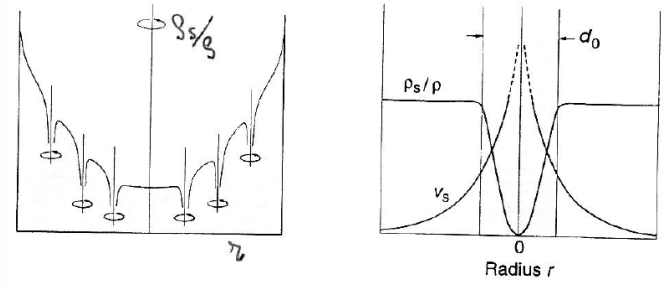
\includegraphics[width=0.7\linewidth]{Immagini - Capitolo 1/vortici He SF.png}
    \caption{formazione dei vortici nell'elio superfluido in rotazione.}
    \label{fig: vortici He SF}
\end{figure}
La conseguenza è che quando si ruota un superfluido si creano dei buchi, come mostrato in figura \ref{fig: vortici He SF}. Un vortice con simmetria cilindrica di questo tipo è descritto da un campo di velocità 
\begin{equation}
    \vv_S(\vr) = (v_x,v_y) = \frac{k}{2\pi r^2}(-y,x)\Rightarrow v_S = \frac{k}{2\pi r} = (\SI{1.58}{\meter\per\second})\times\frac{n}{r}.
\end{equation}
Si può stimare il diametro $d_0$ del nucleo del vortice ponendo
\begin{equation}
    v_S(d_0/2) \simeq v_c(rotone) \simeq \SI{60}{\meter\per\second}.
\end{equation}
In questo modo si trova un valore per $d_0$ dell'ordine di qualche angstrom, cioè dell'ordine delle distanze interatomiche. Il raggio del nucleo del vortice si chiama anche lunghezza di contrazione, che può crescere per $T \simeq T_\Lambda$. 

L'energia $E_v$ per unità di lunghezza di un vortice può essere calcolata integrando l'energia cinetica per unità di volume associata alla rotazione di $\rho_S$ 
\begin{equation}
    E_v = \int_{a_0}^b dr\,\frac{\rho_S v_S^2}{2}2\pi r,
\end{equation}
dove $a_0 \simeq d_0/2$ e $b$ è la metà della distanza tra i vortici o il raggio $R$ del recipiente in rotazione. Poiché $v_S = k/2\pi r$ con $k = nh/m$ si ha
\begin{equation}
    \begin{split}
        E_v = \int_{a_0}^b dr\,\frac{\rho_S k^2}{4\pi r} &= \frac{k^2\rho_S}{4\pi}\log{\frac{b}{a_0}} \\
        &= \frac{n^2h^2\rho_S}{4\pi m^2}\log{\frac{b}{a_0}} \\
        &= \pi n^2\rho_S\bigg(\frac{\hbar}{m}\bigg)^2\log{\frac{b}{a_0}},
    \end{split}
\end{equation}
da cui si vede che $E_v \propto n^2$ e la creazione di molti vortici con vorticità minima con $n = 1$ è energeticamente favorita rispetto, ad esempio, alla creazione di un unico vortice macroscopico centrale con vorticità $k = nh/m$. L'asse del vortice non è necessariamente una retta, ma una linea che può terminare sulle pareti del contenitore o richiudersi su se stessa dando origine a vortici ad anello. Questi vortici sono soluzioni ad energia finita delle equazioni del moto dell'elio superfluido. A causa della quantizzazione della circuitazione di $\vv_S$ queste soluzioni sono stabili e quindi non perdono energia per dissipazione. I vortici si possono creare attraverso l'introduzione di un eccesso di carica tramite elettroni, questi vengono intrappolati nel nucleo del vortice e tramite un campo elettrico si possono raccogliere sulla superficie. I vortici tendono a formare un reticolo triangolare detto ``reticolo di Abriskov''. Per capire come fa a formarsi un vortice quantizzato in un fluido irrotazionale, si può pensare di avere inizialmente due parti di superfluido separate da una sottile parete di fluido normale. Le due parti viaggiano parallele a velocità diverse. Sono due sistemi separati e le funzioni d'onda $\phi_A(x)$ e $\phi_B(x)$ differiscono di una fase. Si supponga che siano in fase a $x = 0$ per cui $\phi_A(0) = \phi_B(0) = \phi_0$, allora
\begin{equation}
    \phi_A(x) = \phi_0\exp{\bigg(\frac{i\hbar}{m}\int_0^x \vv_{S,A}\cdot d\vl\bigg)},\quad \phi_B(x) = \phi_0,
\end{equation}
quindi $\phi_A(x) = \phi_B(x)$ ogni volta che 
\begin{equation}
    \exp{\bigg(\frac{i\hbar}{m}\int_0^x \vv_{S,A}\cdot d\vl\bigg)} = e^{i2\pi n} = 1,
\end{equation}
ossia lungo i cammini chiusi in figura \ref{fig: circuiti He SF}. 
\begin{figure}
    \centering
    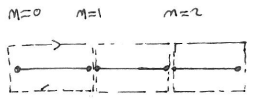
\includegraphics[width=0.4\linewidth]{Immagini - Capitolo 1/circuiti He SF.png}
    \caption{cammini chiusi percorsi dal superfluido.}
    \label{fig: circuiti He SF}
\end{figure}
La circuitazione lungo tali cammini è quantizzata e si può formare il vortice e il fluido normale all'interno può formare il suo nucleo. Vortici con vorticità opposta tendono a respingersi, mentre quelli con stessa vorticità tendono ad avvicinarsi dato che la pressione tra i due non è massima a causa della velocità non nulla del flusso tra i due. L'anello si muove in una direzione perpendicolare al suo piano ad una velocità $\vv_0$ di modulo
\begin{equation}
    v_0 = \frac{\hbar n}{2mr_0},\quad n \in \Z.
\end{equation}
Per ottenere questo valore, si ricorda che un vortice possiede un campo di velocità $v = k/2\pi r = \hbar/rm$ se si considera solo il caso $n = 1$, per cui considerando una sezione del vortice ad anello, come mostrato in figura \ref{fig: sezione toro He SF}, si ha
\begin{equation}
    v_A = \frac{2\hbar}{mr_0} - v_0,\quad v_B = \frac{\hbar}{mr_0} + v_0,
\end{equation}
quindi per non collassare il vortice ad anello deve muoversi verso il basso in modo che la velocità in $A$ e in $B$ siano uguali senza il verificarsi dell'effetto Magnus
\begin{equation}
    \frac{2\hbar}{mr_0} - v_0 = \frac{\hbar}{mr_0} + v_0 \Rightarrow v_0 = \frac{\hbar}{2mr_0}.
\end{equation}
\begin{figure}[h]
    \centering
    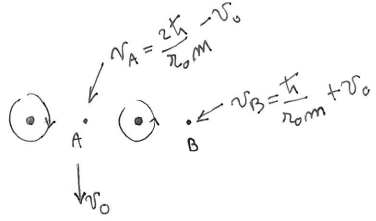
\includegraphics[width=0.5\linewidth]{Immagini - Capitolo 1/sezione toro He SF.png}
    \caption{sezione del vortice toroidale di elio superfluido.}
    \label{fig: sezione toro He SF}
\end{figure}

L'energia trasportata dal vortice si può calcolare approssimativamente applicando la formula del vortice a simmetria cilindrica per un anello di lunghezza $l = 2\pi r$ con
\begin{equation}
    \epsilon(r) = 2\pi r E_v(r) = \frac{k^2\rho_S}{2}r\log{\frac{r}{a_0}}.
\end{equation}
Quando l'elio scorre con velocità $\vv_S$ lungo un capillare di raggio $R$ può produrre dei vortici di raggio $r < R$ purché la valga la condizione di Landau
\begin{equation}
    v_S \ge v_c = \min_q\bigg\{\frac{\epsilon(q)}{q}\bigg\}.
\end{equation}
Per determinare l'impulso $q$ del vortice si usa il fatto che la derivata di $\epsilon(q)$ rispetto a $q$ coincide con la velocità di gruppo della corrispondente quasi-particella, quindi
\begin{equation}
    \frac{d\epsilon}{dq} = v = \frac{\hbar}{2mr},
\end{equation}
da cui 
\begin{equation}
    \frac{dq}{d\epsilon} = \frac{dq}{dr}\frac{dr}{d\epsilon} = \frac{2mr}{\hbar} \Rightarrow \frac{dq}{dr} = \frac{2mr}{\hbar}\frac{d\epsilon}{dr},
\end{equation}
ma d'altra parte si ha
\begin{equation}
    \frac{d\epsilon}{dr} = \frac{k^2\rho_S}{2}\log{\bigg(\frac{r}{a_0}\bigg)} + \frac{k^2\rho_S}{2} = \frac{k^2\rho_S}{2}\bigg[\log{\bigg(\frac{r}{a_0}\bigg)} + 1\bigg],
\end{equation}
che integrata tra $a_0 = d_0/2$ e la metà della distanza tra due vortici $r_0$ usando la relazione
\begin{equation}
    \int_0^r dx\,x\log{x} = \frac{1}{4}\int_0^r dx^2\,\log{x^2} = \frac{r^2}{2}\log{(r)} - \frac{r^2}{4},
\end{equation}
restituisce
\begin{equation}
    \begin{split}
        q &= \frac{k^2\rho_Sm}{\hbar}\int_{a_0}^{r_0}dr\,[r\log{(r)} + r(1 - \log{a_0})] \\
        &= \frac{k^2\rho_Sm}{\hbar}\bigg[\frac{r_0^2}{2}\log{(r_0)} - \frac{r_0^2}{4} - \frac{a_0^2}{2}\log{(a_0)} + \frac{a_0^2}{4} + \frac{r_0^2}{2} \\
        &- \frac{r_0^2}{2}\log{(a_0)} - \frac{a_0^2}{2} + \frac{a_0^2}{2}\log{a_0}\bigg] \\
        &= \frac{k^2\rho_Sm}{\hbar}\bigg[\frac{r_0^2}{2}\log{\bigg(\frac{r_0}{a_0}\bigg)} + \frac{r_0^2}{4} - \frac{a_0^2}{4}\bigg] \\
        &\simeq \frac{k^2\rho_Sm}{\hbar}\bigg[\frac{r_0^2}{2}\log{\bigg(\frac{r_0}{a_0}\bigg)} + \frac{r_0^2}{4}\bigg],
    \end{split}
\end{equation}
dove nell'ultimo passaggio si è trascurato il termine proporzionale a $a_0^2$ dato che $a_0 \ll 1$. Quindi, si ottiene
\begin{equation}
    \frac{\epsilon(r_0)}{q(r_0)} = \frac{\hbar}{mr_0}\frac{\log{(r_0/a_0)}}{\log{(r_0/a_0)} + 1/2} \overset{r_0 \gg a_0}{\simeq} \frac{\hbar}{mr_0},
\end{equation}
la quale ha un minimo per $r_0 \to R$, dunque la velocità critica è
\begin{equation}
    v_c = \frac{\hbar}{mR}\frac{\log{(R/a_0)}}{\log{(R/a_0)} + 1/2}.
\end{equation}
Si formano vortici ad anello delle dimensioni del capillare con una velocità di qualche $\mathrm{mm\,s^{-1}}$ in capillari di circa $\SI{1}{\milli\meter}$ di diametro. 

\subsection{L'equazione di Schr\"odinger non lineare}
L'equazione di Schr\"odinger a molti corpi associata al gas di bosoni è quella introdotta nell'equazione \eqref{eq: equazione di Schrodinger per un gas di bosoni} con hamiltoniana data da \eqref{eq: hamiltoniana per un gas di bosoni}, dove la funzione d'onda è simmetrica per permutazioni dei suoi argomenti come mostrato in equazione \eqref{eq: simmetria per permutazioni della funzione d'onda di un gas di bosoni}. Assumendo l'approssimazione di Hartree-Fock si ha un risultato simile a quello trovato in equazione \eqref{eq: approssimazione di Hartree-Fock per un gas di bosoni} dato da
\begin{equation}
    \phi(\vr_1,\dots,\vr_N) = \prod_{i=1}^N \frac{\phi(\vr_i,t)}{\sqrt{N}},
\end{equation}
con normalizzazione data da
\begin{equation}
    \int d^3r\,\phi^*(\vr,t)\phi(\vr,t) = N.
\end{equation}
La differenza è che adesso tutte le particelle non sono necessariamente nello stato fondamentale, anche se effettivamente l'idea è quella che $\phi(\vr,t)$ descriva solo la componente superfluida e che quindi $N \equiv N_0$ e $\phi(\vr,t) \equiv \phi_0(\vr,t)$. Si definisce l'energia media del sistema come
\begin{equation}
    E = \int d^3r_1\cdots d^3r_N\,\phi^*(\vr_1,\dots,\vr_N)\hatH_N\phi(\vr_1,\dots,\vr_N) = T + V_{ext} + V.
\end{equation}
Quindi, si calcolano 
\begin{equation}
    \begin{split}
        T &= \sum_{i=1}^N \int d^3r_i \frac{\phi^*(\vr_i,t)}{\sqrt{N}}\bigg(-\frac{\hbar^2}{2m}\nabla_{r_i}^2\bigg)\frac{\phi(\vr_i,t)}{\sqrt{N}}\prod_{i\neq j}^N\int d^3r_j\,\frac{\phi^*(\vr_j,t)}{\sqrt{N}}\frac{\phi(\vr_j,t)}{\sqrt{N}} \\
        &= \int d^3r\,\phi^*(\vr,t)\bigg(-\frac{\hbar^2}{2m}\nabla^2\bigg)\phi(\vr,t),
    \end{split}
\end{equation}
analogamente
\begin{equation}
    V_{ext} = \int d^3r\,\phi^*(\vr,t)V_{ext}(\vr)\phi(\vr,t)
\end{equation}
e anche
\begin{equation}
    \begin{split}
        V &= \frac{1}{2}\frac{N(N-1)}{N^2}\int d^3r\,d^3r'\,\phi^*(\vr,t)\phi^*(\vr',t)V(|\vr - \vr'|)\phi(\vr',t)\phi(\vr,t) \\
        &\simeq \frac{1}{2}\int d^3r\,d^3r'\,\phi^*(\vr,t)\phi^*(\vr',t)V(|\vr - \vr'|)\phi(\vr',t)\phi(\vr,t).
    \end{split}
\end{equation}
Per trovare l'equazione del moto si deve definire l'azione 
\begin{equation}
    \action = \int dt\bigg\{\bigg[\int d^3r\,\phi^*(\vr,t)\bigg(i\hbar\frac{\p}{\p t}\bigg)\phi(\vr,t)\bigg] - (T + V_{ext} + V)\bigg\}
\end{equation}
e poi minimizzarla imponendo la condizione
\begin{equation}
    \frac{\delta\action}{\delta\phi^*} = 0\quad\vee\quad \frac{\delta\action}{\delta\phi} = 0. 
\end{equation}
In questo modo si ottiene un'equazione di Schr\"odinger non lineare
\begin{equation}
\label{eq: equazione di schrodinger non lineare}
    i\hbar\frac{\p}{\p t}\phi(\vr,t) = \bigg[-\frac{\hbar^2}{2m}\nabla^2 + V_{ext}(\vr) + \int d^3r'\,\phi^*(\vr',t)V(|\vr - \vr'|)\phi(\vr',t)\bigg]\phi(\vr,t),
\end{equation}
che può essere risolta sotto alcune approssimazioni, oppure tramite metodi numerici. 

Il caso generale con autointerazione $V(|\vr - \vr'|)$ non locale si può solo trattare numericamente, ci si concentra sul caso in cui
\begin{equation}
    V(|\vr - \vr'|) = g\delta(\vr - \vr'),
\end{equation}
il quale porta all'equazione di Gross-Pitaevskii
\begin{equation}
\label{eq: equazione di Gross-Pitaevskii}
    i\hbar\frac{\p}{\p t}\phi(\vr,t) = \bigg[-\frac{\hbar^2}{2m}\nabla^2 + V_{ext}(\vr) + g|\phi(\vr,t)|^2\bigg]\phi(\vr,t).
\end{equation}
L'equazione \eqref{eq: equazione di Gross-Pitaevskii} descrive un sistema a molti corpi in approssimazione di campo medio. L'azione di Gross-Pitaevskii è
\begin{equation}
\label{eq: azione di Gross-Pitaevskii}
    \action_{GP} = -\iint dt\,d^3r \bigg(-i\hbar\phi^*\frac{\p\phi}{\p t} + \frac{\hbar^2}{2m}|\nabla\phi|^2 + V_{ext}(\vr)|\phi|^2 + \frac{g}{2}|\phi|^4\bigg).
\end{equation}
L'equazione di Gross-Pitaevskii stazionaria si ottiene sostituendo\footnote{L'evoluzione temporale di $\phi(\vr,t)$ si giustificherà dal potenziale chimico $\mu = \p_NE$ e non da $E$ quando si parlerà in seguito di stati coerenti.} $\phi(\vr,t) = \phi(\vr)e^{-i\mu t/\hbar}$ nella \eqref{eq: equazione di Gross-Pitaevskii}, quindi si ha
\begin{equation}
    \bigg[-\frac{\hbar^2}{2m}\nabla^2 + V_{ext}(\vr) + g|\phi(\vr)|^2\bigg]\phi(\vr) = \mu\phi(\vr),
\end{equation}
dove per semplicità si pone nel seguito $V_{ext}(\vr) = 0$. L'equazione di Gross-Pitaevskii stazionaria si ottiene anche minimizzando l'energia a fissato numero di particelle ponendo
\begin{equation}
    \frac{\delta}{\delta\phi^*}(E - \mu N) = 0,
\end{equation}
dove 
\begin{equation}
    N = \int d^3r\,\phi^*(\vr)\phi(\vr),\quad E = \int d^3r\bigg(\frac{\hbar^2}{2m}|\nabla\phi|^2 + \frac{g}{2}|\phi|^4\bigg).
\end{equation}
L'equazione \eqref{eq: equazione di Gross-Pitaevskii} può essere considerata l'equivalente delle equazioni di Maxwell dell'elettromagnetismo dove $\phi$ gioca il ruolo del campo elettromagnetico. Nell'equazione di compare $\hbar$ questo è legato alla diversa legge di dispersione $E = cp$, oppure $\omega = ck$, tra fotoni e particelle relativistiche. Con la seconda quantizzazione si passa dall'equazione di Gross-Pitaevskii \eqref{eq: equazione di Gross-Pitaevskii} all'equazione di Schr\"odinger a molti corpi \eqref{eq: equazione di schrodinger non lineare} originaria. Poiché la fase della funzione d'onda macroscopica è diversa da zero, ma l'azione \eqref{eq: azione di Gross-Pitaevskii} ha simmetria $U(1)$ per rotazioni di gauge globali 
\begin{equation}
    \phi(\vr,t) \to \phi(\vr,t)e^{i\alpha},
\end{equation}
tale simmetria deve essere spontaneamente rotta; si vedrà con la condensazione di Bose-Einstein e la comparsa contemporanea di eccitazioni fononiche, è legata alla rottura spontanea di simmetria $U(1)$. 

\subsection{Rottura spontanea di simmetria}
Si è interessati alla soluzione dell'equazione di Gross-Pitaevskii con $\phi(\vr) = \phi_0 \equiv \mathrm{costante}$ che minimizza l'energia $E$ ad un fissato numero di particelle data da
\begin{equation}
    E - \mu N = V\bigg(\frac{g}{2}|\phi_0|^4 - \mu|\phi_0|^2\bigg),
\end{equation}
il cui andamento, mostrato in figura \ref{fig: potenziale sombrero}, ha la peculiare forma di ``cappello messicano''. Il minimo si ha quindi per
\begin{equation}
    \frac{\delta(E - \mu N)}{\delta|\phi_0|^2} = 0,
\end{equation}
che restituisce la relazione
\begin{equation}
    |\phi_0|^2 = \frac{\mu}{g} = \frac{\rho_0}{m} = n_0,
\end{equation}
cioè la fase di $\phi_0$ è arbitraria mentre il modulo è fisso. 
\begin{figure}[h]
    \centering
    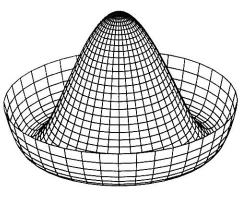
\includegraphics[width=0.3\linewidth]{Immagini - Capitolo 1/potenziale sombrero.png}
    \caption{andamento del potenziale a cappello messicano.}
    \label{fig: potenziale sombrero}
\end{figure}
In questo modo si trova la relazione tra il potenziale chimico, la costante di accoppiamento $g$ e la densità delle particelle con
\begin{equation}
    \mu = \frac{g\rho_0}{m} = g|\phi_0|^2.
\end{equation}
In conclusione, l'azione della teoria possiede una simmetria globale $U(1)$ poiché è invariante sotto l'aggiunta di un fattore costante nella fase della funzione d'onda. Lo stato fondamentale non possiede invece questa simmetria; infatti, la teoria prevede un continuo di vuoti degeneri e la funzione d'onda macroscopica per lo stato fondamentale
\begin{equation}
    \phi(\vr) \equiv \phi_0 = |\phi_0|e^{i\alpha},
\end{equation}
che ha una fase ben definita. Per un sistema relativisticamente invariante è abbastanza semplice dimostrare che esistono due tipi di eccitazioni legate al meccanismo della rottura spontanea di simmetria $U(1)$:
\begin{enumerate}
    \item un bosone a massa nulla, detto ``bosone di Goldstone'', associato a variazioni di fase della funzione d'onda;

    \item un bosone massivo, detto ``bosone di Anderson-Higgs, associato ad oscillazioni nel modulo $\phi$.
\end{enumerate}
Nel caso non relativistico è più complessa e conviene analizzare il problema in dettaglio.

\subsection{Pseudo-particelle di Bogoljubov}
Una classe importante dell'equazione di Gross-Pitaevskii \eqref{eq: equazione di Gross-Pitaevskii} corrisponde ad oscillazioni di piccola ampiezza dove le variazioni nello spazio e nel tempo di $\phi$, rispetto alla configurazione omogenea $\phi_0$, sono piccole
\begin{equation}
    \phi(\vr,t) = [\phi_0 + \theta(\vr,t)]e^{-i\mu t/\hbar},\quad |\phi_0|^2 = \frac{\mu}{g} = \frac{N_0}{V},
\end{equation}
dove ci si pone in $T = \SI{0}{\kelvin}$ e si trascura il fenomeno dello svuotamento quantistico. Si pone quindi
\begin{equation}
    \theta(\vr,t) = u_ke^{i(\vk\cdot\vr - \omega t)} + v_ke^{-i(\vk\cdot\vr - \omega t)},
\end{equation}
per cui 
\begin{equation}
    \begin{split}
        \phi(\vr,t) &= \phi_0e^{-i\mu t/\hbar} + [u_ke^{i[\vk\cdot\vr - (\omega + \mu/\hbar) t]} + v_ke^{-i(\vk\cdot\vr - (\omega - \mu/\hbar) t)}] \\
        &\equiv \phi_0e^{-i\mu t/\hbar} + \delta\phi,
    \end{split}
\end{equation}
che si sostituisce nell'equazione
\begin{equation}
\label{eq: equazione di schrodinger non lineare con Vext = 0 e V = g*delta}
    i\hbar\frac{\p}{\p t}\phi(\vr,t) + \frac{\hbar^2}{2m}\nabla^2\phi(\vr,t) = g|\phi(\vr,t)|^2\phi(\vr,t).
\end{equation}
Il contributo al primo ordine del membro di sinistra della \eqref{eq: equazione di schrodinger non lineare con Vext = 0 e V = g*delta} è
\begin{equation}
    \bigg[(\hbar\omega + \mu) - \frac{\hbar^2k^2}{2m}\bigg]u_ke^{i[\vk\cdot\vr - (\omega + \mu/\hbar)t]} + \bigg[(\mu - \hbar\omega) - \frac{\hbar^2k^2}{2m}\bigg]v_ke^{-i[\vk\cdot\vr - (\omega - \mu/\hbar)t]},
\end{equation}
dove si è trascurato il termine costante $\mu\phi_0$. Ponendo
\begin{equation}
    \phi(\vr,t) = \phi_0e^{-i\mu t/\hbar} + \delta\phi,\quad \phi^*(\vr,t) = \phi_0e^{i\mu t/\hbar} + \delta\phi^*,
\end{equation}
si ha
\begin{equation}
    \begin{split}
        g|\phi|^2\phi &= g(\phi_0e^{-i\mu t/\hbar} + \delta\phi)(\phi_0e^{i\mu t/\hbar} + \delta\phi^*)(\phi_0e^{-i\mu t/\hbar} + \delta\phi) \\
        &= g\phi_0^3e^{-i\mu t/\hbar} + 2g\phi_0^2\delta\phi + g\phi_0^2e^{-2i\mu t/\hbar}\delta\phi^* + O(\delta\phi^2);
    \end{split}
\end{equation}
trascurando il termine costante $g\phi_0^3e^{-i\mu t/\hbar}$, il termine di ordine $O(\delta\phi)$ è
\begin{equation}
    \begin{split}
        2\mu\delta\phi + \mu e^{-2i\mu t/\hbar}\delta\phi^* &= 2\mu(u_ke^{i[\vk\cdot\vr - (\omega + \mu/\hbar)t]} + v_ke^{-i[\vk\cdot\vr - (\omega - \mu/\hbar)t]}) \\
        &+ \mu e^{-2i\mu t/\hbar}(u_k^*e^{-i[\vk\cdot\vr - (\omega + \mu/\hbar)t]} + v_ke^{i[\vk\cdot\vr - (\omega - \mu/\hbar)t]}) \\
        &= \mu(2u_k + v_k^*)e^{i[\vk\cdot\vr - (\omega + \mu/\hbar)t]} \\
        &+ \mu(2v_k + u_k^*)e^{-i[\vk\cdot\vr - (\omega - \mu/\hbar)t]},
    \end{split}
\end{equation}
arrivando infine al sistema 
\begin{equation}
    \begin{cases}
        \bigg[(\hbar\omega + \mu) - \dfrac{\hbar^2k^2}{2m}\bigg]u_k = 2\mu u_k + \mu v_k^* \\[2ex]
        \bigg[(\mu - \hbar\omega) - \dfrac{\hbar^2k^2}{2m}\bigg]v_k^* = 2\mu v_k^* + \mu u_k
    \end{cases},
\end{equation}
il quale può essere riscritto in forma matriciale come
\begin{equation}
    \begin{pmatrix}
        \hbar\omega - \mu - \dfrac{\hbar^2k^2}{2m} & -\mu \\
        -\mu & -\mu - \hbar\omega - \dfrac{\hbar^2k^2}{2m}
    \end{pmatrix}
    \begin{pmatrix}
        u_k \\
        v_k^*
    \end{pmatrix}
    = 0.
\end{equation}
Questo sistema di equazioni risulta in soluzioni non banali se e solo se 
\begin{equation}
    \det{
    \begin{pmatrix}
        \hbar\omega - \mu - \dfrac{\hbar^2k^2}{2m} & -\mu \\
        -\mu & -\mu - \hbar\omega - \dfrac{\hbar^2k^2}{2m}
    \end{pmatrix}
    } = 0,
\end{equation}
da cui, tramite il calcolo esplicito
\begin{equation}
    \begin{split}
        \bigg(\hbar\omega - \mu - \frac{\hbar^2k^2}{2m}\bigg)\bigg(-\mu - \hbar\omega - \frac{\hbar^2k^2}{2m}\bigg) - \mu^2& = 0 \\
        \bigg[- \hbar^2\omega^2 + \bigg(\mu + \frac{\hbar^2k^2}{2m}\bigg)^2\bigg] - \mu^2 &= 0 \\
        \bigg(\mu + \frac{\hbar^2k^2}{2m}\bigg)^2 - \mu^2 &= \hbar^2\omega^2,
    \end{split}
\end{equation}
si può ricavare la relazione di dispersione di Bogoljubov
\begin{equation}
\label{eq: relazione di dispersione di Bogoljubov}
    \hbar\omega = \sqrt{\frac{\hbar^2k^2}{2m}\bigg(\frac{\hbar^2k^2}{2m} + 2\mu\bigg)}\quad\Longleftrightarrow\quad \epsilon(k) = \sqrt{\epsilon_0(k)[\epsilon_0(k) + 2\mu]}.
\end{equation}
\begin{obs}
    La relazione che si troverebbe al posto della \eqref{eq: relazione di dispersione di Bogoljubov} considerando il segno opposto quando si prende la radice ambo i membri corrisponde allo scambio $u_k\longleftrightarrow v_{-k}$: le due soluzioni rappresentano lo stesso tipo di oscillazione fisica.
\end{obs}
Considerando il limite in cui $k \to 0$ nella relazione trovata in \eqref{eq: relazione di dispersione di Bogoljubov} si ha 
\begin{equation}
    \hbar\omega \equiv \epsilon(k) \simeq \sqrt{\frac{\mu}{m}}\hbar k = v_1 q,\quad v_1 = \sqrt{\frac{\mu}{m}} = \sqrt{\frac{gn_0}{m}},
\end{equation} 
dove $v_1$ è la velocità del fonone. Quindi, la pseudo-particella di Bogoljubov corrispondente a questa legge di dispersione è un caso particolare di bosone di Goldstone per un condensato di particelle bosoniche debolmente interagenti. Invece, nel limite $k \to \infty$ si ha 
\begin{equation}
    \epsilon(k) = \epsilon_0(k)\sqrt{1 + \frac{2\mu}{\epsilon_0(k)}} \simeq \epsilon_0(k) + \mu,
\end{equation}
quindi la legge di dispersione tende asintoticamente, a meno della costante $\mu$, a quella di particella libera. In conclusione, l'interazione caratterizzata dal parametro $g > 0$ è responsabile della rottura spontanea di simmetria e della comparsa delle eccitazioni di Bogoljubov. Compare una ibridizzazione tra la curva di dispersione fononica e quella di particella libera, come mostrato in figura \ref{fig: e(q) regime fononico}.
\begin{figure}[h]
    \centering
    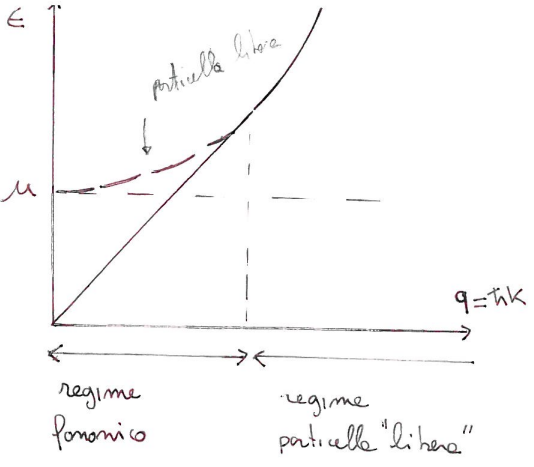
\includegraphics[width=0.4\linewidth]{Immagini - Capitolo 1/e(q) regime fononico.png}
    \caption{confronto tra le relazioni di dispersione nei regimi di particelle libera e fononico.}
    \label{fig: e(q) regime fononico}
\end{figure}
La funzione $\theta(\vr,t)$ può corrispondere ad oscillazioni di fase e modulo: non esiste una pseudo-particella di Anderson-Higgs distinta dal bosone di Goldstone nei condensati di Bose-Einstein.

\subsection{Solitone}
Si considerano ora delle soluzioni dell'equazione di Gross-Pitaevskii dipendente dal tempo che prendono il nome di  ``solitoni''. Nel caso repulsivo dove $g > 0$, queste soluzioni corrispondono a modulazioni della densità localizzate che si muovono nel condensato con velocità costante e preservando la loro forma nel tempo. Il profilo del solitone nella regione perturbata è caratterizzato da una diminuzione della densità $\rho_0$ rispetto al valore di bulk e si chiama ``solitone grigio''. L'esistenza di quest'ultimo è direttamente legata alla non linearità dell'equazione di Gross-Pitaevskii, il cui effetto compensa il termine quantistico di pressione associato all'energia cinetica. L'estensione spaziale del solitone è caratterizzata dalla lunghezza di ``healing'' $\xi$ definita come
\begin{equation}
\label{eq: lunghezza di healing}
    \xi = \frac{\hbar}{\sqrt{2m gn_0}},\quad n_0 = \frac{N_0}{V} \equiv \frac{N}{V}.
\end{equation}
Quindi, si ritorna all'equazione \eqref{eq: equazione di schrodinger non lineare con Vext = 0 e V = g*delta}, che si riporta qui per comodità 
\begin{equation}
    i\hbar\frac{\p}{\p t}\phi(\vr,t) = \bigg[-\frac{\hbar^2}{2m}\nabla^2 + g|\phi(\vr,t)|^2\bigg]\phi(\vr,t),
\end{equation}
e si considerano soluzioni che descrivono la propagazione di un fronte d'onda perpendicolare all'asse $z$, ossia della forma 
\begin{equation}
\label{eq: ansatz soluzione di solitone}
    \phi(\vr,t) = \sqrt{n_0}f(z,t)e^{-i\mu t/\hbar} \equiv \phi_s(\vr,t)e^{-i\mu t/\hbar},
\end{equation}
dove $f(z,t)$ è una funzione che dipende solo dalla coordinata cartesiana $z$. Quindi, sostituendo l'ansatz \eqref{eq: ansatz soluzione di solitone} nell'equazione \eqref{eq: equazione di schrodinger non lineare con Vext = 0 e V = g*delta} si ha
\begin{equation}
    \begin{split}
        i\hbar\frac{\p f(z,t)}{\p t} + \mu f(z,t) &= \bigg[-\frac{\hbar^2}{2m}\frac{\p^2}{\p z^2} + gn_0|f(z,t)|^2\bigg]f(z,t) \\
        i\hbar\frac{\p}{\p t}f(z,t) &= \bigg[-\frac{\hbar^2}{2m}\frac{\p^2}{\p z^2}f(z,t) + gn_0(|f(z,t)|^2 - 1)f(z,t)\bigg],
    \end{split}
\end{equation}
di cui si cercano soluzioni del tipo $f(z,t) \equiv f(z - vt)$. Con questa assunzione si trova
\begin{equation}
    -\frac{i\hbar v}{gn_0}\frac{df(z - vt)}{d(z - vt)} = -\frac{\hbar^2}{2mgn_0}\frac{d^2}{d(z - vt)^2}f(z - vt) + (|f(z - vt)|^2 - 1)f(z - vt),
\end{equation}
che definendo il parametro $\gamma$ tramite la lunghezza di healing, definita in equazione \eqref{eq: lunghezza di healing}, come
\begin{equation}
    \gamma \equiv \frac{z - vt}{\xi},
\end{equation}
diventa 
\begin{equation}
    -\frac{i\hbar v}{gn_0}\frac{\sqrt{2mgn_0}}{\hbar}\frac{df(\gamma)}{d\gamma} = -\frac{d^2f(\gamma)}{d\gamma^2} + (|f(\gamma)|^2 - 1)f(\gamma).
\end{equation}
Adesso, considerando che la velocità del suono $v_1$ nel condensato è pari a $v_1 = \sqrt{gn_0/m}$, si pone 
\begin{equation}
    \frac{v}{gn_0}\sqrt{2mgn_0} = \sqrt{2}v\sqrt{\frac{m}{gn_0}} = \sqrt{2}\frac{v}{v_1} \equiv 2U.
\end{equation}
Dunque, l'equazione che si deve risolvere è
\begin{equation}
\label{eq: equazione solitone in gamma}
    2iU\frac{df}{d\gamma} = \frac{d^2f}{d\gamma^2} + (1 - |f|^2)f,
\end{equation}
con l'obiettivo di trovare una soluzione localizzata che soddisfi le condizioni asintotiche
\begin{equation}
\label{eq: condizioni al bordo del solitone}
    \begin{cases}
        |f(\gamma)| \to 1 \\[2ex]
        \dfrac{df}{d\gamma} \to 0
    \end{cases},\quad \gamma \to \pm\infty.
\end{equation}
Per farlo, si moltiplica l'equazione appena trovata \eqref{eq: equazione solitone in gamma} per $f^*(\gamma)$ e se ne sottrae la complessa coniugata moltiplicata per $f$, ossia da 
\begin{equation}
    \begin{cases}
        2iUf^*\dfrac{df}{d\gamma} = f^*\dfrac{d^2f}{d\gamma^2} + (1 - |f^2|)|f^2| \\
        -2iUf\dfrac{df^*}{d\gamma} = f\dfrac{d^2f^*}{d\gamma^2} + (1 - |f^2|)|f^2|
    \end{cases}
\end{equation}
si ottiene
\begin{equation}
    2iU\bigg(f^*\frac{df}{d\gamma} + f\frac{df^*}{d\gamma}\bigg) = f^*\dfrac{d^2f}{f\gamma^2} - f\frac{d^2f^*}{d\gamma^2},
\end{equation}
la quale integrata in $d\gamma'$ sull'intervallo $\gamma' \in [\gamma,\infty]$ restituisce
\begin{equation}
\label{eq: equazione di continuità del solitone}
    2iU(1 - |f|^2) + f^*\frac{df}{d\gamma} - f\frac{df^*}{d\gamma} = 0,
\end{equation}
del tutto consistente con le condizioni al bordo imposte in \eqref{eq: condizioni al bordo del solitone}.
\begin{obs}
    Non è un caso che l'equazione \eqref{eq: equazione di continuità del solitone} abbia la forma di un'equazione di continuità, infatti il procedimento seguito per ottenerla è il medesimo usato in Meccanica quantistica per ottenere proprio l'equazione di continuità.
\end{obs}
Adesso, è possibile ottenere un'altra equazione a partire dalla \eqref{eq: equazione solitone in gamma} considerandone la parte immaginaria
\begin{equation}
    2U\frac{df_1}{d\gamma} = \frac{d^2f_2}{d\gamma^2} + (1 - f_1^2 - f_2^2)f_2,\quad f = f_1 + if_2,
\end{equation}
della quale si intende cercare soluzioni con $f_2 = \mathrm{costante}$, per cui l'equazione si riduce semplicemente a
\begin{equation}
\label{eq: equazione parte immaginaria solitone I}
    \frac{2U}{f_2}\frac{df_1}{d\gamma} = (1 - f_1^2 - f_2^2),
\end{equation}
sotto questa stessa assunzione l'equazione di continuità \eqref{eq: equazione di continuità del solitone} diventa 
\begin{equation}
    \begin{split}
        -2iU(1 - f_1^2 - f_2^2) &= (f_1 - if_2)\frac{d}{d\gamma}(f_1 + if_2) - (f_1 + if_2)\frac{d}{d\gamma}(f_1 - if_2) \\
        &= -2if_2\frac{df_1}{d\gamma},
    \end{split}
\end{equation}
ossia
\begin{equation}
\label{eq: equazione parte immaginaria solitone II}
    \frac{f_2}{U}\frac{df_1}{d\gamma} = (1 - f_1^2 - f_2^2).
\end{equation}
Le equazioni \eqref{eq: equazione parte immaginaria solitone I} e \eqref{eq: equazione parte immaginaria solitone II} coincidono se e solo se 
\begin{equation}
\label{eq: condizione su f2 per concidenza equazioni I e II}
    \frac{2U}{f_2} = \frac{f_2}{U}\quad\Longrightarrow\quad f_2 = \sqrt{2}U \equiv \frac{v}{v_1}.
\end{equation}
Quindi, sostituendo la condizione \eqref{eq: condizione su f2 per concidenza equazioni I e II} in una delle due equazioni si ha
\begin{equation}
    \sqrt{2}\dfrac{df_1}{d\gamma} = \bigg(1 - \frac{v^2}{v_1^2} - f_1^2\bigg),
\end{equation}
che può essere riscritta nella forma 
\begin{equation}
    \frac{d}{d\bigg(\gamma\sqrt{\dfrac{1 - v^2/v_1^2}{2}}\bigg)}\bigg(\frac{f_1}{\sqrt{1 - v^2/v_1^2}}\bigg) = \bigg[ 1 - \bigg(\frac{f_1}{\sqrt{1 - v^2/v_1^2}}\bigg)^2\bigg],
\end{equation}
così da poterla confrontare con la relazione generale
\begin{equation}
    \frac{d}{dx}\tanh{(x)} = 1 - \tanh^2{(x)}
\end{equation}
e ottenendo infine
\begin{equation}
\label{eq: soluzione f1 del solitone}
    f_1 = \sqrt{1 - \frac{v^2}{v_1^2}}\tanh{\bigg(\gamma\sqrt{\frac{1 - v^2/v_1^2}{2}}\bigg)}.
\end{equation}
Dunque, sostituendo l'espressione trovata per $f_1$ \eqref{eq: soluzione f1 del solitone} nell'ansatz originario \eqref{eq: ansatz soluzione di solitone} si ottiene la soluzione del solitone grigio
\begin{equation}
\label{eq: soluzione del solitone grigio}
    \phi_s(z - vt) = \sqrt{n_0}\bigg[\frac{iv}{v_1} + \sqrt{1 - \frac{v^2}{v_1^2}}\tanh{\bigg(\frac{z - vt}{\sqrt{2}\xi}\sqrt{1 - \frac{v^2}{v_1^2}}\bigg)}\bigg].
\end{equation}
Il profilo di densità $n(z - vt) = |\phi_s(z - vt)|^2$ ha la forma di una campana capovolta, come mostrato in figura \ref{fig: profilo densità solitone grigio}. Il minimo di questa funzione corrisponde alla condizione $z - vt = 0$, ossia a $\tanh{(0)} = 0$, che risulta nel valore
\begin{equation}
    n(0) = n_0\bigg|\frac{iv}{v_1}\bigg|^2 = n_0\frac{v^2}{v_1^2}. 
\end{equation}
\begin{obs}
    Per un solitone con velocità $v = 0$, ovvero per il quale il minimo del profilo di densità è $n(0) = 0$, si parla di ``dark soliton''.
\end{obs}
\begin{figure}[h]
    \centering
    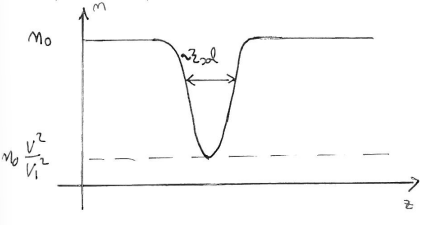
\includegraphics[width=0.5\linewidth]{Immagini - Capitolo 1/profilo densità solitone grigio.png}
    \caption{profilo di densità relativo alla soluzione del solitone grigio.}
    \label{fig: profilo densità solitone grigio}
\end{figure}
La fase della funzione d'onda subisce una variazione finita tra $z = -\infty$ e $z = \infty$, infatti partendo da
\begin{align}
    \phi_s(\infty) = i\sqrt{n_0}\bigg(\frac{v}{v_1} - i\sqrt{1 - \frac{v^2}{v_1}}\bigg), \\
    \phi_s(-\infty) = i\sqrt{n_0}\bigg(\frac{v}{v_1} + i\sqrt{1 - \frac{v^2}{v_1}}\bigg),
\end{align}
si può calcolare il rapporto 
\begin{equation}
    \frac{\phi_s(\infty)}{\phi_s(-\infty)} = e^{i\Delta\phi} = \bigg(\frac{v}{v_1} - i\sqrt{1 - \frac{v^2}{v_1^2}}\bigg)^2,
\end{equation}
da cui si trova che la differenza di fase è 
\begin{equation}
    \Delta\phi = 2\arccos{\bigg(\frac{v}{v_1}\bigg)}.
\end{equation}
\begin{obs}
    Per un ``dark soliton'' $\phi_s$ è reale e dispari, quindi la differenza di fase è pari a $\Delta\phi = \pi$, che corrisponde ad un ``difetto topologico'', ossia il fluido viene diviso a metà da uno strato di fluido in fase normale.
\end{obs}
La ``larghezza'' del solitone, mostrata in figura \ref{fig: profilo densità solitone grigio}, è legata alla lunghezza di healing tramite la relazione
\begin{equation}
    \xi_s = \frac{\xi}{\sqrt{1 - v^2/v_1^2}},
\end{equation}
la quale tende a divergere ad $\infty$ nel limite $v \to v_1$. Ora, è possibile calcolare l'energia del solitone per unità di superficie $\epsilon_s$ come
\begin{equation}
    \begin{split}
        \epsilon_s &= \int_\R dz\,\bigg[\frac{\hbar^2}{2m}\bigg|\frac{d\phi_s}{dz}\bigg|^2 + \bigg(\frac{g}{2}|\phi_s|^4 - gn_0|\phi_s|^2\bigg)\bigg] - \bigg(\frac{g}{2}|\phi_0|^4 - gn_0|\phi_0|^2\bigg). \\
        &= \int_\R dz\,\bigg[\frac{\hbar^2}{2m}\bigg|\frac{d\phi_s}{dz}\bigg|^2 + \frac{g}{2}(|\phi_s|^2 - n_0)^2\bigg],
    \end{split}
\end{equation}
dove il termine nella seconda parentesi tonda corrisponde all'energia dello stato imperturbato, per cui la differenza tra i due termini nelle tonde è la differenza tra le energie grancanoniche in presenza e in assenza del solitone; ad ogni modo, da questo, svolgendo l'integrale, si trova
\begin{equation}
    \epsilon_s = \frac{4}{3}\hbar v_1n_0\bigg( 1 - \frac{v^2}{v_1^2}\bigg)^{3/2}.
\end{equation}
Nel limite in cui $v \ll 1$, l'energia $\epsilon_s$ può essere espansa come
\begin{equation}
    \epsilon_s \simeq \frac{4}{3}\hbar v_1 n_0 - 2\hbar v_1 n_0 \frac{v^2}{v_1^2} = \frac{4}{3}\hbar v_1 n_0 + \frac{1}{2}\bigg(-\frac{4\hbar n_0}{v_1}\bigg)v^2,
\end{equation}
quindi il solitone si comporta come una particella di massa negativa
\begin{equation}
    m_s = -\frac{4\hbar n_0}{v_1},
\end{equation}
in accordo con il fatto che la modulazione di densità corrisponde ad una ``buca'' piuttosto che ad una ``particella''. Un fatto particolare, è che la velocità del solitone aumenta al decrescere dell'energia, questo vuole dire che in presenza di dissipazione dovuta alle collisioni con fononi a temperature $T > \SI{0}{\kelvin}$ il solitone accelera fino ad eventualmente scomparire quando $v \to v_1$. Quindi, il solitone è instabile per fluttuazioni nelle direzioni trasverse, per questo negli esperimenti con atomi freddi l'instabilità viene soppressa diminuendo le dimensioni trasversali tramite trappole magnetiche.

\section{Quantizzazione canonica}
Da un punto di vista formale, la Meccanica quantistica può essere interpretata come una deformazione della Meccanica classica, in cui le variabili classiche vengono sostituite da operatori che al posto di comparire nelle parentesi di Poisson compaiono nell'anticommutatore rispettivo. Quindi, date due variabili classiche $f$ e $g$ con la relazione
\begin{equation}
    \acomm{f}{g} = \sum_{i=1}^s\bigg(\frac{\p f}{\p q^i}\frac{\p g}{\p p_i} - \frac{\p f}{\p p_i}\frac{\p g}{\p q^i}\bigg),
\end{equation}
dove $s$ indica il numero di gradi di libertà del sistema, il passaggio alla trattazione quantistica consiste nel promuovere $f$ e $g$ al ruolo di operatori hermitiani $\hatf$ e $\hatg$, rispettivamente, e di definire una relazione di commutazione analoga alle parentesi di Poisson
\begin{equation}
     \acomm{f}{g} \xrightarrow{MQ} \frac{1}{i\hbar}\comm{\hatf}{\hatg} = \frac{1}{i\hbar} \sum_{i=1}^s\bigg(\frac{\p \hatf}{\p q^i}\frac{\p \hatg}{\p p_i} + \frac{\p \hatf}{\p p_i}\frac{\p \hatg}{\p q^i}\bigg),
\end{equation}
dove $\{q^i\}$ e $\{p_i\}$ sono le variabili canonicamente coniugate, ossia tali che
\begin{equation}
    \acomm{q^k}{p_j} = \sum_{i=1}^s\bigg(\frac{\p q_k}{\p q^i}\frac{\p p_j}{\p p_i} - \frac{\p q_k}{\p p_i}\frac{\p p_j}{\p q^i}\bigg) = \delta_{kj} \xrightarrow{MQ} \comm{\hatq_k}{\hatp_j} = i\hbar\delta_{kj}.
\end{equation}
L'evoluzione classica di una funzione $f$ è data da
\begin{equation}
    \frac{df}{dt} = \frac{\p f}{\p t} + \sum_{i=1}^s\bigg(\frac{\p f}{\p q^i}\frac{\p H}{\p p_i} - \frac{\p f}{\p p_i}\frac{\p H}{\p q^i}\bigg) = \frac{\p f}{\p t} + \acomm{f}{H} \xrightarrow{MQ} \frac{d\hatf}{dt} = \frac{\p\hatf}{\p t} + \comm{\hatf}{\hatH},
\end{equation}
dove $H(\vq,\vp)$ è l'hamiltoniana del sistema in Meccanica classica che soddisfa le equazioni di Hamilton
\begin{equation}
    \begin{cases}
        \dfrac{\p H}{\p p_i} = \dot{q}^i \\[2ex]
        \dfrac{\p H}{\p q^i} = -\dot{p}_i
    \end{cases},
\end{equation}
mentre $\hatH$ è l'operatore hamiltoniano in Meccanica quantistica. Si può poi introdurre la Lagrangiana del sistema come
\begin{equation}
    \dL(q_i,\dot{q}_i) = \sum_{i=1}^sp_i\dot{q}^i - H(\vq,\vp),
\end{equation}
da cui si definisce il momento canonicamente coniugato a $q^i$ come
\begin{equation}
    p_i = \frac{\p \dL}{\p \dot{q}^i}.
\end{equation}

\subsection{Oscillatore armonico come teoria di campo}
Si consideri l'hamiltoniana dell'oscillatore armonico 
\begin{equation}
\label{eq: hamiltoniana oscillatore armonico}
    H(\phi,\pi) = \frac{\pi(t)^2}{2m} + \frac{m\omega^2}{2}\phi(t)^2,
\end{equation}
dove $\phi$ e $\pi$ sono variabili canonicamente coniugate dalle relazioni
\begin{equation}
    \frac{\p H}{\p \pi} = \frac{\pi(t)}{m} = \dot{\phi}(t),\quad \frac{\p H}{\p \phi} = m\omega^2\phi(t) = -\dot{\pi}(t).
\end{equation}
In generale, esistono due modi per quantizzare il sistema dell'oscillatore armonico. Inizialmente, si può pensare di promuovere le variabili coniugate $\phi(t)$ e $\pi(t)$ al ruolo di operatori $\hatphi(t)$ e $\hatpi(t)$ con le relazioni di commutazione $\comm{\hatphi}{\hatpi} = i\hbar$ dove si passa
\begin{equation}
    \pi(t) \to \hatpi(t) = -i\hbar\frac{\p}{\p \phi},\quad \phi(t) \to \hatphi(t),
\end{equation}
in questo modo si arriva all'equazione di Schr\"odinger 
\begin{equation}
    \bigg(-\frac{\hbar^2}{2m}\frac{\p^2}{\p \phi^2} + \frac{m\omega}{2}\phi^2\bigg)\Psi(\phi,t) = i\hbar\frac{\p}{\p t}\Psi(\phi,t).
\end{equation}
Questo formalismo può essere utilizzato anche in una teoria di campo, ossia quando $\phi(\vr,t)$ dipende da un indice continuo $\vr$; tuttavia, è una tecnica non molto popolare a causa della perdita esplicita, nel caso di teorie invarianti relativistiche, della covarianza e delle difficoltà tecniche associate ad una trattazione rigorosa di equazioni alle derivate funzionali. In alternativa, si può dividere il campo $\phi(t)$ in due ``campi'' complessi
\begin{equation}
    \begin{cases}
        \phi(t) = \sqrt{\dfrac{\hbar}{2m\omega}}[a(t) + a^*(t)] \\[2ex]
        \pi(t) = \sqrt{\dfrac{m\omega\hbar}{2}}[a(t) - a^*(t)]
    \end{cases},
\end{equation}
da cui si ricavano le relazioni inverse
\begin{equation}
    \begin{cases}
        a(t) = \dfrac{i}{\sqrt{2\hbar m\omega}}\pi(t) + \sqrt{\dfrac{m\omega}{2\hbar}}\phi(t) \\
        a^*(t) = -\dfrac{i}{\sqrt{2\hbar m\omega}}\pi(t) + \sqrt{\dfrac{m\omega}{2\hbar}}\phi(t)
    \end{cases},
\end{equation}
che possono essere usate per riscrivere l'hamiltoniana nella \eqref{eq: hamiltoniana oscillatore armonico} come
\begin{equation}
    \begin{split}
        H &= \hbar\omega\bigg(-\dfrac{i}{\sqrt{2\hbar m\omega}}\pi(t) + \sqrt{\dfrac{m\omega}{2\hbar}}\phi(t)\bigg)\bigg(\dfrac{i}{\sqrt{2\hbar m\omega}}\pi(t) + \sqrt{\dfrac{m\omega}{2\hbar}}\phi(t)\bigg) \\
        &= \hbar\omega a^*(t)a(t).
    \end{split}
\end{equation}
Non è complesso vedere che il cambiamento di variabili $\{\phi,\pi\} \to i\hbar\{a,a^*\}$ corrisponde ad una trasformazione canonica
\begin{equation}
    \begin{split}
        i\hbar\acomm{a}{a^*} &= i\hbar\bigg(\frac{\p a}{\p \phi}\frac{\p a^*}{\p \pi} - \frac{\p a}{\p \pi}\frac{\p a^*}{\p \phi}\bigg) \\
        &= \bigg(-\dfrac{i}{\sqrt{2\hbar m\omega}}\sqrt{\dfrac{m\omega}{2\hbar}} -\dfrac{i}{\sqrt{2\hbar m\omega}}\sqrt{\dfrac{m\omega}{2\hbar}}\bigg) \\
        &= 1,
    \end{split}
\end{equation}
per quantizzare la teoria quindi si passa da
\begin{equation}
    i\hbar\acomm{a}{a^*} = 1 \xrightarrow{MQ} \comm{\hata}{\hataT} = 1,
\end{equation}
con la quale si può riscrivere l'operatore hamiltoniano come
\begin{equation}
    \hatH = \hbar\omega\bigg(\hataT\hata + \frac{1}{2}\bigg) \equiv \hbar\omega\bigg(\hatN + \frac{1}{2}\bigg),
\end{equation}
dove $\hatN := \hataT\hata$ è l'operatore numero che fornisce, tramite la sua equazione agli autovalori $\hatN\ket{N} = N\ket{N}$, il numero di quanti $N$. In Teoria dei campi l'idea è di identificare le particelle del sistema come gli autostati dell'hamiltoniana quantistica, ossia con le eccitazioni del campo ad energia definita, per cui gli operatori $\hata$ e $\hataT$ possono essere interpretati come gli operatori di distruzione di stati di particella con energia $\hbar\omega$ e di creazione di stati di particella con la medesima energia. Questi operatori agiscono su stati appartenenti ad uno spazio di Fock a numero finito di particelle; quindi, indicando con $\ko$ lo stato di vuoto, gli operatori si definiscono in modo che 
\begin{equation}
    \hata\ko = 0,\quad \hataT\ko = \ket{1},
\end{equation}
o su uno stato di $N$ particelle
\begin{equation}
    \hata\ket{N} = \sqrt{N}\ket{N - 1},\quad \hataT\ket{0} = \sqrt{N!}\ket{N}.
\end{equation}

\subsection{Quantizzazione dell'equazione di Gross-Pitaevskii}
L'equazione di Gross-Pitaevskii in seconda quantizzazione si ottiene, come nel caso dell'oscillatore armonico, individuando coppie di variabili classiche canonicamente coniugate e promuovendole al rango di operatori. La densità di lagrangiana di Gross-Pitaevskii è
\begin{equation}
    \dL_{GP} = i\hbar\phi^*(\vr,t)\frac{\p}{\p t}\phi(\vr,t) - \frac{\hbar^2}{2m}\nabla\phi^*(\vr,t)\nabla\phi(\vr,t) - \frac{g}{2}|\phi(\vr,t)|^4,
\end{equation}
quindi il momento coniugato a $\phi$ è 
\begin{equation}
    \pi(\vr,t) = \frac{\p \dL}{\p(\p_t\phi)} = i\hbar\phi^*(\vr,t).
\end{equation}
Promuovendo $\phi(\vr,t)$ e $\pi(\vr,t)$ ad operatori si definiscono le relazioni di commutazione a tempi uguali tra i due campi
\begin{equation}
\label{eq: relazioni di commutazione per campi bosonici}
    \begin{cases}
        \comm{\hatphi(\vr,t)}{\hatphid(\vr',t)} = \delta(\vr' - \vr) \\
        \comm{\hatphi(\vr,t)}{\hatphi(\vr',t)} = 0 \\ 
        \comm{\hatphid(\vr,t)}{\hatphid(\vr',t)} = 0
    \end{cases},
\end{equation}
da cui si capisce che i campi $\phi(\vr,t)$ e $\pi(\vr,t)$ seguono la statistica di Bose-Einstein. Se si definisce lo stato fondamentale $\kO$, allora il campo di creazione agisce su di esso come
\begin{equation}
    \hatphid(\vr)\kO = \ket{\vr},
\end{equation}
ovvero creando una particella con coordinate spaziali $\vr$; in modo analogo, lo stato a due particelle è dato da
\begin{equation}
    \frac{1}{\sqrt{2}}\hatphid(\vr_1)\hatphid(\vr_2)\kO = \ket{\vr_1,\vr_2} = \frac{1}{\sqrt{2}}\hatphid(\vr_2)\hatphid(\vr_1)\kO = \ket{\vr_2,\vr_1},
\end{equation}
che risulta essere simmetrico per lo scambio delle particelle dato che la statistica è quella bosonica. In generale, lo stato ad $N$ particella è completamente simmetrico sotto lo scambio di qualsiasi coppia di particelle ed è dato da
\begin{equation}
    \ket{\vr_1,\dots,\vr_N} = \frac{1}{\sqrt{N!}}\hatphid(\vr_1)\cdots\hatphid(\vr_N)\kO.
\end{equation}
L'hamiltoniana di Gross-Pitaevskii in seconda quantizzazione è
\begin{equation}
    \hatH_{GP} = \int d^3r\bigg[\hatphid(\vr)\bigg(-\frac{\hbar^2}{2m}\nabla^2\bigg)\hatphi(\vr) + \frac{g}{2}\hatphid(\vr)^2\hatphi(\vr)^2\bigg],
\end{equation}
la quale agisce sullo stato fondamentale annichilandolo, ossia $\hatH_{GP}\kO = 0$. Un generico stato fisico $\ket{\Phi(t)}$ deve essere una soluzione dell'equazione di Schr\"odinger 
\begin{equation}
    i\hbar\frac{\p}{\p t}\ket{\Phi(t)} = \hatH_{GP}\ket{\Phi(t)}.
\end{equation}
Si calcola ora il commutatore dell'hamiltoniana $\hatH_{GP}$ con il campo $\hatphid(\vr)$
\begin{equation}
    \begin{split}
        \comm{\hatH_{GP}}{\hatphid(\vr)} &= \int d^3r_1\bigg[\hatphid(\vr_1)\bigg(-\frac{\hbar^2}{2m}\nabla^2_{\vr_1}\bigg)\hatphi(\vr_1) + \frac{g}{2}\hatphid(\vr)^2\hatphi(\vr)^2,\hatphid(\vr)\bigg] \\
        &= \int d^3r_1\bigg\{-\frac{\hbar^2}{2m}\nabla^2_{\vr_1}\hatphid(\vr_1)\comm{\hatphi(\vr_1)}{\hatphid(\vr)} \\
        &+ g\hatphid(\vr_1)^2\hatphi(\vr_1)\comm{\hatphi(\vr_1)}{\hatphid(\vr)}\bigg\} \\
        &= -\frac{\hbar^2}{2m}\nabla^2\hatphid(\vr) + g\hatphid(\vr)^2\hatphi(\vr),
    \end{split}
\end{equation}
dove si sono usate nell'ultimo passaggio le relazioni di commutazioni definite nella \eqref{eq: relazioni di commutazione per campi bosonici}; quindi il commutatore cercato vale
\begin{equation}
\label{eq: commutatore H_GP e phiT}
    \comm{\hatH_{GP}}{\hatphid(\vr)} = \bigg[-\frac{\hbar^2}{2m}\nabla^2 + g\hatphid(\vr)\hatphi(\vr)\bigg]\hatphid(\vr),
\end{equation}
con il quale si può scrivere l'equazione di Gross-Pitaevskii per il campo $\hatphid$ come
\begin{equation}
\label{eq: equazione di Gross-Pitaevskii per campo phiT}
    i\hbar\frac{\p}{\p t}\hatphid(\vr) = -\comm{\hatH_{GP}}{\hatphid(\vr)}.
\end{equation}

\subsubsection{Stato ad una particella}
Ci consideri ora lo stato ad una particella $\ket{\vr} = \hatphid(\vr)\kO$ e se ne calcoli la norma
\begin{equation}
    \begin{split}
        \mybraket{\vr_1}{\vr} = \mybrakett{\Omega}{\hatphi(\vr_1)\hatphid(\vr)}{\Omega} &= \mybrakett{\Omega}{\comm{\hatphi(\vr_1)}{\hatphid(\vr)}}{\Omega} \\
        &= \mybrakett{\Omega}{\delta(\vr_1 - \vr)}{\Omega} \\
        &= \delta(\vr_1 - \vr),
    \end{split}
\end{equation}
mentre la relazione di completezza è
\begin{equation}
    \int d^3r\,\ket{\vr}\bra{\vr} = \MI.
\end{equation}
Uno stato fisico $\ket{\Phi(t)}$ ad una particella può essere quindi rappresentato utilizzando la base $\{\vr\}$ come
\begin{equation}
    \ket{\Phi(t)} = \int d^3r\,\ket{\vr}\mybraket{\vr}{\Phi(t)} = \int d^3r\,\Phi(\vr,t)\ket{\vr},
\end{equation}
dove $\Phi(\vr,t)$ è la funzione che determina la particolare sovrapposizione di autostati di posizione $\ket{\vr}$ che compongono $\ket{\Phi(t)}$. Si vuole ora dimostrare che $\Phi(\vr,t)$ soddisfa l'equazione di Schr\"odinger della particella libera 
\begin{equation}
\label{eq: equazione di schrodinger della particella libera}
    i\hbar\frac{\p}{\p t}\Phi(\vr,t) = -\frac{\hbar^2}{2m}\nabla^2\Phi(\vr,t);
\end{equation}
per farlo si calcola esplicitamente
\begin{equation}
    \begin{split}
        i\hbar\frac{\p}{\p t}\ket{\Phi(t)} &= \int d^3r\bigg(i\hbar\frac{\p}{\p t}\Phi(\vr,t)\bigg)\ket{\vr} \\
        &= \hatH_{GP}\ket{\Phi(\vr,t)} \\
        &= \int d^3r\,\Phi(\vr,t)\hatH_{GP}\hatphid(\vr)\kO \\
        &= \int d^3r\,\Phi(\vr,t)\comm{\hatH_{GP}}{\hatphid(\vr)}\kO \\
        &= \int d^3r\,\Phi(\vr,t)\bigg[-\frac{\hbar^2}{2m}\nabla^2\hatphid(\vr) + g\hatphid(\vr)^2\hatphi(\vr)\bigg]\kO \\
        &= \int d^3r\bigg(-\frac{\hbar^2}{2m}\nabla^2\bigg)\Phi(\vr,t)\hatphid(\vr)\kO \\
        &= \int d^3r\bigg(-\frac{\hbar^2}{2m}\nabla^2\Phi(\vr,t)\bigg)\ket{r},
    \end{split}
\end{equation}
dove nel secondo passaggio si è usata l'equazione \eqref{eq: equazione di Gross-Pitaevskii per campo phiT}, nel quarto si è usata la relazione \eqref{eq: commutatore H_GP e phiT} e infine nel quinto si è integrato due volte per parti in modo ``da spostare'' l'operatore $\nabla^2$; quindi, confrontando gli integrandi nel primo e nell'ultimo passaggio si trova direttamente quanto volevasi dimostrare
\begin{equation}
    i\hbar\frac{\p}{\p t}\Phi(\vr,t) = -\frac{\hbar^2}{2m}\nabla^2\Phi(\vr,t).
\end{equation}

\subsubsection{Stato a due particelle}
Si consideri ora lo stato a due particelle 
\begin{equation}
    \ket{r_1,r_2} = \frac{1}{\sqrt{2}}\hatphid(\vr_1)\hatphid(\vr_2)\kO
\end{equation}
e se ne calcoli la norma 
\begin{equation}
    \begin{split}
        \mybraket{r_1,r_2}{r_1',r_2'} &= \frac{1}{2}\mybrakett{\Omega}{\hatphi(\vr_1)\hatphi(\vr_2)\hatphid(\vr_1')\hatphid(\vr_2')}{\Omega} \\
        &= \frac{1}{2}\mybrakett{\Omega}{\hatphi(\vr_2)\{\comm{\hatphi(\vr_1)}{\hatphid(\vr_1')} + \hatphid(\vr_1')\hatphi(\vr_1)\}\hatphid(\vr_2')}{\Omega} \\
        &= \frac{1}{2}\mybrakett{\Omega}{\hatphi(\vr_2)[\delta(\vr_1 - \vr_1') + \hatphid(\vr_1')\hatphi(\vr_1)]\hatphid(\vr_2')}{\Omega} \\
        &= \frac{1}{2}\mybrakett{\Omega}{\hatphi(\vr_2)\delta(\vr_1 - \vr_1')\hatphid(\vr_2')}{\Omega} \\
        &+ \frac{1}{2}\mybrakett{\Omega}{\hatphi(\vr_2)\hatphid(\vr_1')\comm{\hatphi(\vr_1)}{\hatphid(\vr_2')}}{\Omega} \\
        &= \frac{1}{2}\delta(\vr_1 - \vr_1')\delta(\vr_2 - \vr_2') + \frac{1}{2}\delta(\vr_2 - \vr_1')\delta(\vr_1 - \vr_2').
    \end{split}
\end{equation}
Questa norma suggerisce che si sta studiando un sistema a due particelle identiche, infatti la norma è diversa da zero se e solo se
\begin{equation}
    \begin{cases}
        r_1 = r_1' \\
        r_2 = r_2'
    \end{cases}
    \quad \vee \quad\quad
    \begin{cases}
        r_1 = r_2' \\
        r_2 = r_1'
    \end{cases}.
\end{equation}
Un generico stato $\ket{\Phi(t)}$ a due particelle può quindi essere sviluppato sulla base $\ket{r_1,r_2}$ come
\begin{equation}
    \begin{split}
        \ket{\Phi(t)} &= \int d^3r_1\,d^3r_2\, \Phi(\vr_1,\vr_2,t)\ket{\vr_1,\vr_2} \\
        &= \frac{1}{\sqrt{2}}\int d^3r_1\,d^3r_2\,\Phi(\vr_1,\vr_2,t)\hatphid(\vr_1)\hatphid(\vr_2)\kO,
    \end{split}
\end{equation}
dove, poiché $\comm{\hatphid(\vr_1)}{\hatphid(\vr_2)} = 0$, l'integrale su $r_1$ e $r_2$ è simmetrico sotto lo scambio $(\vr_1 \longleftrightarrow \vr_2)$ quindi $\Phi(\vr_1,\vr_2,t) = \Phi(\vr_2,\vr_1,t)$ e si ha
\begin{equation}
\label{eq: equazione di schrodinger a due particelle}
    i\hbar\frac{\p}{\p t}\ket{\Phi(t)} = \int d^3r_1\,d^3r_2\,\bigg[i\hbar\frac{\p}{\p t}\Phi(\vr_1,\vr_2,t)\bigg]\ket{\vr_1,\vr_2}.
\end{equation}
A destra dell'equazione di Schr\"odinger \eqref{eq: equazione di schrodinger a due particelle} si ha
\begin{equation}
    \begin{split}
        \hatH_{GP}\ket{\Phi(t)} &= \frac{1}{\sqrt{2}}\int d^3r_1\,d^3r_2\,\Phi(\vr_1,\vr_2,t)\hatH_{GP}\hatphid(\vr_1)\hatphid(\vr_2)\kO \\
        &= \frac{1}{\sqrt{2}}\int d^3r_1\,d^3r_2\,\Phi(\vr_1,\vr_2,t) \\ &\times(\comm{\hatH_{GP}}{\hatphid(\vr_1)} + \hatphid(\vr_1)\hatH_{GP})\hatphid(\vr_2)\kO \\
        &= \frac{1}{\sqrt{2}}\int d^3r_1\,d^3r_2\bigg[-\frac{\hbar^2}{2m}\nabla^2_{\vr_1}\hatphid(\vr_1) + g\hatphid(\vr_1)^2\hatphi(\vr_1)\bigg] \\
        &\times\Phi(\vr_1,\vr_2,t)\hatphid(\vr_2)\kO + \frac{1}{2}\int d^3r_1\,d^3r_2\,\Phi(\vr_1,\vr_2,t)\hatphid(\vr_1) \\
        &\times\comm{\hatH_{GP}}{\hatphid(\vr_2)}\kO,
    \end{split}
\end{equation}
dove nell'ultimo passaggio si è usato che $\hatH_{GP}\kO = 0$, ora integrando per parti il primo termine si ha
\begin{equation}
    \begin{split}
        \hatH_{GP}\ket{\Phi(t)} &= \frac{1}{\sqrt{2}}\int d^3r_1\,d^3r_2\bigg[\hatphid(\vr_1)\bigg(-\frac{\hbar^2}{2m}\nabla^2_{\vr_1}\bigg) + g\hatphid(\vr_1)^2\hatphi(\vr_1)\bigg] \\
        &\times\Phi(\vr_1,\vr_2,t)\hatphid(\vr_2)\kO + \frac{1}{\sqrt{2}}\int d^3r_1\,d^3r_2\,\hatphid(\vr_1)\Phi(\vr_1,\vr_2,t) \\
        &\times\bigg[-\frac{\hbar^2}{2m}\nabla^2_{\vr_2}\hatphid(\vr_2) + g\hatphid(\vr_2)^2\hatphi(\vr_2)\bigg]\kO \\
        &= \frac{1}{\sqrt{2}}\int d^3r_1\,d^3r_2\bigg[-\frac{\hbar^2}{2m}\nabla^2_{\vr_1}\Phi(\vr_1,\vr_2,t)\bigg]\hatphid(\vr_1)\hatphid(\vr_2)\kO \\
        &+ \frac{1}{\sqrt{2}}\int d^3r_1\,d^3r_2\, g\hatphid(\vr_1)^2\delta(\vr_1 - \vr_2)\Phi(\vr_1,\vr_2,t)\kO \\
        &+ \frac{1}{\sqrt{2}}\int d^3r_1\,d^3r_2\,\bigg[-\frac{\hbar^2}{2m}\nabla^2_{\vr_2}\Phi(\vr_1,\vr_2,t)\bigg]\hatphid(\vr_1)\hatphid(\vr_2)\kO \\
        &= \int d^3r_1\,d^3r_2\bigg[-\frac{\hbar^2}{2m}\nabla^2_{\vr_1} -\frac{\hbar^2}{2m}\nabla^2_{\vr_2}\bigg]\Phi(\vr_1,\vr_2,t)\ket{\vr_1,\vr_2} \\
        &+ \int d^3r_1\,d^3r_2\,g\delta(\vr_1 - \vr_2)\Phi(\vr_1,\vr_2,t)\ket{\vr_1,\vr_2},
    \end{split}
\end{equation}
dove si è usata la proprietà $\hatphid(\vr_1)^2\delta(\vr_1 - \vr_2) = \hatphid(\vr_1)\hatphid(\vr_2)\delta(\vr_1 - \vr_2)$ e integrato per parti nel secondo passaggio. Finalmente, si arriva a 
\begin{multline}
    \int d^3r_1\,d^3r_2\,\bigg[i\hbar\frac{\p}{\p t}\Phi(\vr_1,\vr_2,t)\bigg]\ket{\vr_1,\vr_2} = \\ = \int d^3r_1\,d^3r_2\bigg[-\frac{\hbar^2}{2m}\nabla^2_{\vr_1} -\frac{\hbar^2}{2m}\nabla^2_{\vr_2} + g\delta(\vr_1 - \vr_2)\bigg]\Phi(\vr_1,\vr_2,t)\ket{\vr_1,\vr_2},
\end{multline}
la quale porta all'equazione di Schr\"odinger a due corpi con un potenziale a delta di Dirac
\begin{equation}
    i\hbar\frac{\p}{\p t}\Phi(\vr_1,\vr_2,t) = \bigg[-\frac{\hbar^2}{2m}\nabla^2_{\vr_1} -\frac{\hbar^2}{2m}\nabla^2_{\vr_2} + g\delta(\vr_1 - \vr_2)\bigg]\Phi(\vr_1,\vr_2,t).
\end{equation}
Nel caso di un sistema ad $N$ particelle, lo stato è dato da
\begin{equation}
    \ket{\Phi(t)} = \frac{1}{\sqrt{N!}}\int d^3r_1\cdots d^3r_N\,\Phi(\vr_1,\dots,\vr_N,t)\hatphid(\vr_1)\cdots\hatphid(\vr_N)\kO.
\end{equation}
\begin{obs}
    Un risultato simile si sarebbe potuto ottenere anche con un potenziale generico $V(\vr_1 - \vr_2)$.
\end{obs}
In conclusione, si è dimostrato che l'hamiltoniana in seconda quantizzazione $\hatH_{GP}$, quando ristretta ad un sottospazio con $N$ fissato, è equivalente ad un'equazione di Schr\"odinger a molti corpi con un interazione descritta dalla delta di Dirac e della statistica bosonica. Per sistemi non relativistici la ``seconda quantizzazione'' è solo un modo più conveniente per formulare la Meccanica quantistica a molti corpi. In Meccanica quantistica relativistica il numero di particelle non è in generale conservato e il formalismo della seconda quantizzazione è l'unico utilizzabile.
\begin{center}
    \begin{tikzpicture}[
        box/.style = {rectangle, draw, rounded corners=2mm, thin, minimum width=2.5cm, minimum height=1.4cm, align=center}, node distance=2.5cm]
        \node[box] (a) {Equazione di Schr\"odinger \\ a $N$ corpi con potenziale \\ a delta di Dirac};
        \node[box, right=of a] (b) {Equazione di Gross-Pitaevskii \\ in seconda quantizzazione};
        \node[box, below=of $(a)!0.5!(b)$] (c){Equazione di Gross-Pitaevskii ``classica''};
          
        \draw[<-] (a) -- node[above, align=center]{sottospazio \\ con $N$ fisso } (b);
        \draw[<-] (b) -- node[right=8pt, align=left]{ quantizzazione canonica \\ del campo di G-P} (c);
        \draw[<-] (c) -- node[left=8pt, align=right]{$N \gg 1$ campo medio \\ di Hartree-Fock} (a);
    \end{tikzpicture}
\end{center}

\subsubsection{Operatore numero di particelle}
Il numero di particelle in un determinato stato $\ket{\Phi(t)}$ è un autovalore dell'operatore
\begin{equation}
    \hatN = \int dr\,\hatphid(\vr)\hatphi(\vr),\quad \hatN\kO = 0.
\end{equation}
Calcolando i commutatori
\begin{align}
    \comm{\hatN}{\hatphi(\vr)} = \int dr_1\,\comm{\hatphid(\vr_1)\hatphi(\vr_1)}{\hatphi(\vr)} = -\int dr_1\delta(\vr_1 - \vr)\hatphi(\vr_1) = -\hatphi(\vr), \\
    \comm{\hatN}{\hatphid(\vr)} = \int dr_1\,\comm{\hatphid(\vr_1)\hatphi(\vr_1)}{\hatphid(\vr)} = \int dr_1\delta(\vr_1 - \vr)\hatphid(\vr_1) = \hatphid(\vr),
\end{align}
si possono riscrivere come
\begin{equation}
    \begin{cases}
        \hatN\hatphid(\vr) = \hatphid(\vr)(\hatN + 1) \\
        \hatN\hatphi(\vr) = \hatphi(\vr)(\hatN - 1)
    \end{cases};
\end{equation}
quindi per uno stato ad $N$ particelle si ha
\begin{equation}
    \begin{split}
        \hatN\ket{\vr_1,\dots,\vr_N} &= \frac{1}{\sqrt{N!}}\hatN\hatphid(\vr_1)\cdots\hatphid(\vr_N)\kO \\
        &= \frac{1}{\sqrt{N!}}\hatphid(\vr_1)\cdots\hatphid(\vr_N)(\hatN + N)\kO \\
        &= N\ket{\vr_1,\dots,\vr_N}.
    \end{split}
\end{equation}

\section{Spazio dei momenti}
Risulta probabilmente più intuitivo considerare gli operatori di creazione e distruzione nello spazio dei momenti dato che l'hamiltoniana è diagonale in tale spazio in assenza di un potenziale di interazione. Si supponga che il sistema sia contenuto in un volume $V = L^3$ con condizioni periodiche al bordo, in tal caso si può sviluppare il campo $\hatphi(\vr)$ in serie di Fourier 
\begin{equation}
    \hatphi(\vr) = \frac{1}{\sqrt{V}}\nsum_k\hata_ke^{i\vk\cdot\vr},\quad \vk = \frac{2\pi\hbar}{L}(n_x,n_y,n_z),\quad n_x,n_y,n_z \in \Z,
\end{equation}
per cui la trasformazione inversa è
\begin{equation}
    \hata_k = \frac{1}{\sqrt{V}}\int d^3r\,\hatphi(\vr)e^{-i\vk\cdot\vr},
\end{equation}
con la quale si può calcolare il commutatore
\begin{equation}
    \begin{split}
        \comm{\hata_k}{\hataT_q} &= \frac{1}{V}\int d^3r\,d^3r_1\comm{\hatphi(\vr)e^{-i\vk\cdot\vr}}{\hatphid(\vr)e^{i\vq\cdot\vr_1}} \\
        &= \frac{1}{V}\int d^3r\,d^3r_1\,\delta(\vr - \vr_1)e^{-i\vk\cdot\vr}e^{i\vq\cdot\vr_1} \\
        &= \frac{1}{V}\int d^3r\,e^{i(\vk - \vq)\vr} \\
        &= \delta_{k,q},
    \end{split}
\end{equation}
che corrisponde proprio alla relazione di commutazione canonica tra $\hata$ e $\hataT$ dell'oscillatore armonico; naturalmente, valgono anche le relazioni $\comm{\hata_k}{\hata_q} = \comm{\hataT_k}{\hataT_q} = 0$. Si riscrive quindi l'hamiltoniana $\hatH_{GP}$ nello spazio dei momenti come
\begin{equation}
    \begin{split}
        \hatH_{GP} &= \int d^3r\bigg[\hatphid(\vr)\bigg(-\frac{\hbar^2}{2m}\nabla^2\bigg)\hatphi(\vr) + \frac{g}{2}\hatphid(\vr)^2\hatphi(\vr)^2\bigg] \\
        &\equiv \int d^3r\,(\hatT_{GP} + \hatV_{GP}),
    \end{split}
\end{equation}
dove il termine cinetico è
\begin{equation}
    \begin{split}
        \hatT_{GP} &= \int d^3r\,\hatphid(\vr)\bigg(-\frac{\hbar^2}{2m}\nabla^2\bigg)\hatphi(\vr) \\
        &= \frac{1}{V}\int d^3r\,\sum_{k,q}\hataT_qe^{-iqr}\bigg(-\frac{\hbar^2}{2m}\nabla^2\bigg)\hata_ke^{i\vk\cdot\vr} \\
        &= \sum_{k,q}\hataT_q\hata_k\bigg(\frac{\hbar^2k^2}{2m}\bigg)\frac{1}{V}\int d^3r\,e^{-i(\vq - \vk)\cdot r} \\
        &= \sum_{k,q}\hataT_q\hata_k\bigg(\frac{\hbar^2k^2}{2m}\bigg)\delta_{k,q} \\
        &= \nsum_{k}\frac{\hbar^2k^2}{2m}\hataT_k\hata_k \\
        &\equiv \nsum_{k}\frac{\hbar^2k^2}{2m}\hatN_k,
    \end{split}
\end{equation}
mentre quello di interazione è
\begin{equation}
    \begin{split}
        \hatV_{GP} &= \frac{g}{2}\int d^3r\,\hatphid(\vr)\hatphid(\vr)\hatphi(\vr)\hatphi(\vr) \\
        &= \frac{g}{2V^2}\sum_{\substack{k1,k_2 \\ q_1,q_2}}\int d^3r\,\hataT_{q_2}\hataT_{q_1}\hata_{k_1}\hata_{k_2}e^{i(q_1 + q_2 - k_1 - k_1)r} \\
        &= \frac{g}{2V}\sum_{\substack{k1,k_2 \\ q_1,q_2}}\hataT_{q_2}\hataT_{q_1}\hata_{k_1}\hata_{k_2}\delta_{k_1 + k_2, q_1 + q_2}.
    \end{split}
\end{equation}
Quindi, l'interpretazione dell'hamiltoninana nello spazio dei momenti 
\begin{equation}
\label{eq: hamiltoniana nello spazio dei momenti}
    \hatH_{GP} = \nsum_k\frac{\hbar^2k^2}{2m}\hataT_k\hata_k + \frac{g}{2V}\sum_{\substack{k1,k_2 \\ q_1,q_2}}\hataT_{q_2}\hataT_{q_1}\hata_{k_1}\hata_{k_2}\delta_{k_1 + k_2, q_1 + q_2}
\end{equation}
consiste nelle seguenti osservazioni:
\begin{enumerate}
    \item il termine cinetico $\hatT_{GP}$ è interpretato come l'operatore che conta il numero di particelle con momento $\vk$ e che associa ad ognuna di esse un'energia $\hbar^2k^2/2m$ ;
    \item il termine di potenziale $\hatV_{GP}$ causa la scattering annichilendo due particelle con impulso $\vk_1$ e $\vk_2$ e creandone altre due con impulso $\vq_1$ e $\vq_2$, conservando sempre il momento totale con $\vk_1 + \vk_2 = \vq_1 + \vq_2$.
\end{enumerate}
Usando la conservazione del quadrimpulso codificata dalla $\delta_{k_1 + k_2, q_1 + q_2}$ si può riscrivere il termine di interazione nella \eqref{eq: hamiltoniana nello spazio dei momenti} come
\begin{equation}
    \hatV_{GP} = \frac{g}{2V}\sum_{\substack{k1,k_2 \\ q}}\hataT_{k_2 + q}\hataT_{k_1 - q}\hata_{k_1}\hata_{k_2}.
\end{equation}
\begin{obs}
    Se ci fosse un termine che non conserva il numero di particelle, ad esempio $\hataT\hataT\hataT\hata\hata$, non sarebbe possibile stabilire l'equivalenza con l'equazione di Schr\"odinger a molti corpi. In questi casi la trattazione tramite la Teoria dei campi è l'unica possibile.
\end{obs}

\section{Stati coerenti}
Dalla Meccanica quantistica è noto che lo stato fondamentale dell'oscillatore armonico minimizza il principio di indeterminazione di Heisenberg 
\begin{equation}
    \vmedio{(\Delta\hatphi)^2}_0\vmedio{(\Delta\hatpi)^2}_0 = \frac{\hbar^2}{4},
\end{equation}
dove $\Delta\hatphi = \hatphi - \vmedio{\hatphi}_0 = \hatphi$ e $\Delta\hatpi = \hatpi - \vmedio{\hatpi}_0 = \hatpi$. Non è complesso dimostrare che invece lo stato ad $N$ particelle non minimizza il principio di indeterminazione, infatti
\begin{align}
    \mybrakett{N}{(\hata + \hataT)(\hata + \hataT)}{N} &= \mybrakett{N}{\hata\hataT + \hataT\hata}{N} \notag \\
    &= \mybrakett{N}{2\hataT\hata + \comm{\hata}{\hataT}}{N} \\
    &= 2N + 1, \notag \\
    \mybrakett{N}{(\hata + \hataT)(\hata + \hataT)}{N} &= -(2N + 1),
\end{align}
poiché gli operatori si possono esprimere come
\begin{equation}
    \begin{cases}
        \hata - \hataT = i\sqrt{\dfrac{2}{m\omega\hbar}}\hatpi \\[2ex]
        \hata + \hataT = \sqrt{\dfrac{2m\omega}{\hbar}}\hatphi
    \end{cases}
\end{equation}
si ottiene
\begin{equation}
    \vmedio{(\Delta\hatphi)^2}_N\vmedio{(\Delta\hatpi)^2}_N = \frac{\hbar^2}{4}(2N + 1)^2.
\end{equation}
Questo dimostra che la parte destra dell'uguaglianza dipende da $N$ ed è minima per $N = 0$; quindi, il principio di indeterminazione non è minimizzato se si considerano valori medi sullo stato con numero di particelle fissato. Per il vuoto funziona perché $\hata\ko = 0\ko$, cioè $\ko$ è autostato di $\hata$. Se si considera ora un autostato generico di $\hata$ con autovalore $\alpha \in \C$ definito da
\begin{equation}
    \begin{cases}
        \hata\ket{\alpha} = \alpha\ket{\alpha} \\
        \bra{\alpha}\hataT = \alpha^*\ket{\alpha}
    \end{cases}
    ,\quad \mybraket{\alpha}{\alpha} = 1,
\end{equation}
si hanno $\mybrakett{\alpha}{(\hata + \hataT)}{\alpha} = \alpha + \alpha^*$ e $\mybrakett{\alpha}{(\hata - \hataT)}{\alpha} = \alpha - \alpha^*$ con i quali si calcola
\begin{align}
    \begin{split}
        \mybrakett{\alpha}{(\hata + \hataT)(\hata + \hataT)}{\alpha} &= \mybrakett{\alpha}{\hata^2 + (\hataT)^2 + \hata\hataT + \hataT\hata}{\alpha} \\
        &= \alpha^2 + (\alpha^*)^2 + 2\alpha^*\alpha + 1 \\
        &= (\alpha + \alpha^*)^2 + 1
    \end{split} \\
    \begin{split}
        \mybrakett{\alpha}{(\hata - \hataT)(\hata - \hataT)}{\alpha} &= \mybrakett{\alpha}{\hata^2 + (\hataT)^2 - \hata\hataT - \hataT\hata}{\alpha} \\
        &= \alpha^2 + (\alpha^*)^2 - 2\alpha^*\alpha - 1 \\
        &= (\alpha - \alpha^*)^2 - 1.
    \end{split}
\end{align}
Quindi, si calcolano
\begin{align}
    \begin{split}
        \vmedio{(\Delta\hatphi)^2}_\alpha = \vmedio{\hatphi^2}_\alpha - \vmedio{\hatphi}_\alpha^2 &= \frac{\hbar}{2m\omega}[(\alpha + \alpha^*)^2 + 1 - (\alpha + \alpha^*)^2] \\
        &= \frac{\hbar}{2m\omega},
    \end{split} \\
    \begin{split}
        \vmedio{(\Delta\hatpi)^2}_\alpha = \vmedio{\hatpi^2}_\alpha - \vmedio{\hatpi}_\alpha^2 &= -\frac{m\omega}{2\hbar}[(\alpha - \alpha^*)^2 - 1 - (\alpha - \alpha^*)^2] \\
        &= \frac{m\omega}{2\hbar}.
    \end{split}
\end{align}
Dunque, si ottiene la relazione di indeterminazione
\begin{equation}
\label{eq: principio di indeterminazione}
    \vmedio{(\Delta\hatphi)^2}_\alpha\vmedio{(\Delta\hatpi)^2}_\alpha = \frac{\hbar^2}{4}
\end{equation}
e lo stato $\ket{\alpha}$ minimizza il principio di indeterminazione per ogni $\alpha \in \C$. Il fatto che gli stati coerenti minimizzano il principio di indeterminazione è molto importante perché se si interpreta $\hata$ come il campo $\hatphi$ dell'equazione di Gross-Pitaesvkii, il valore di aspettazione di $\hata$ deve essere diverso da zero, come lo deve essere quello di $\hatphi$, così da poter ottenere $\mybrakett{\alpha}{\hata}{\alpha} = \alpha$.
\begin{obs}
    In questo caso si è posto $t = 0$, ma il risultato finale vale per ogni $t$, in accordo con l'idea che la coerenza viene conservata nel tempo.
\end{obs}
Lo stato coerente $\ket{\alpha}$ può essere rappresentato come somma infinita, con particolari coefficienti, nella base dello spazio di Fock come
\begin{equation}
    \ket{\alpha} = e^{-|\alpha|^2/2}\sum_{N=0}^\infty\frac{\alpha^N}{\sqrt{N!}}\ket{N},
\end{equation}
sul quale può agire l'operatore $\hata$ nel modo seguente
\begin{equation}
    \begin{split}
        \hata\ket{\alpha} &= e^{-|\alpha|^2/2}\sum_{N=1}^\infty\frac{\alpha^N\sqrt{N}}{\sqrt{(N - 1)!\sqrt{N}}}\ket{N - 1} \\
        &= \alpha e^{-|\alpha|^2/2}\sum_{N=1}^\infty\frac{\alpha^{N - 1}}{\sqrt{(N - 1)!}}\ket{N - 1} \\
        &= \alpha\ket{\alpha},
    \end{split}
\end{equation}
o alternativamente come
\begin{equation}
    \begin{split}
        \ket{\alpha} = e^{-(|\alpha|^2/2) + \alpha\hataT}\ko &=  e^{\alpha\hataT - \alpha^*\hata}\ko \\
        &= e^{-|\alpha|^2/2}\sum_{N=0}^\infty\frac{\alpha^N(\hataT)^N}{N!}\ko \\
        &= e^{-|\alpha|^2/2}\sum_{N=0}^\infty\frac{\alpha^N}{\sqrt{N!}}\ket{N},
    \end{split}
\end{equation}
dove nel primo passaggio si è usata la relazione di Baker-Campbell-Hausdorff
\begin{equation}
    e^{\hatA + \hatB} = e^{-\comm{\hatA}{\hatB}/2}e^{\hatA} e^{\hatB},
\end{equation}
che vale solamente se il commutatore dei due operatori commuta con i medesimi operatori singolarmente
\begin{equation}
    \comm{\comm{\hatA}{\hatB}}{\hatA} = \comm{\comm{\hatA}{\hatB}}{\hatB} = 0,
\end{equation}
dove $\hatA$ e $\hatB$ non commutano necessariamente tra di loro. Inoltre, l'evoluzione temporale di $\hata$ è dettata da
\begin{equation}
    \hata(t) = \hata e^{-i\omega t} = \hata e^{-i(\p E/\p N)t/\hbar} \equiv \hata e^{-i\mu t/\hbar},
\end{equation}
dove quindi è il potenziale chimico $\mu$, e non l'energia $E$, a determinare l'evoluzione temporale dello stato coerente. L'operatore 
\begin{equation}
    \hatD(\alpha) := e^{\alpha\hataT - \alpha^*\hata},
\end{equation}
tale che $\hatD(\alpha)\ko = \ket{\alpha}$, è detto operatore di Glauber. Questo operatore è unitario dato che $\hat\hatD(\alpha)\hatD^\dg(\alpha) = \MI$, inoltre usando il lemma di Hadamard
\begin{equation}
    e^{\hatA} e^{\hatB} = \hatB + \comm{\hatA}{\hatB} + \frac{1}{2!}\comm{\hatA}{\comm{\hatA}{\hatB}} + \cdots,
\end{equation}
con $\hatA = \alpha\hataT - \alpha^*\hata$ e $\hatB = \hata$ in modo che $\comm{\hatA}{\hatB} = \alpha$, si trova che
\begin{equation}
    \begin{cases}
        \hatD(\alpha)\hata\hatD(\alpha) = \hata - \alpha \\
        \hatD(\alpha)\hataT\hatD^\dg(\alpha) = \hataT - \alpha^*
    \end{cases};
\end{equation}
quindi, l'operatore di Glauber trasla il campo $\hata$ di un fattore $\alpha$ costante. Due stati coerenti $\ket{\alpha}$ e $\ket{\beta}$ non sono ortogonali, ossia $\mybraket{\alpha}{\beta} \neq 0$ per $\alpha \neq \beta$; infatti lo si può vedere calcolando
\begin{align}
    \begin{split}
        \mybraket{\alpha}{\beta} &= e^{-|\alpha|^2/2}e^{-|\beta|^2/2}\nsum_N\nsum_{N'}\frac{(\alpha^*)^N(\beta)^{N'}}{\sqrt{N!}\sqrt{N'!}}\mybraket{N}{N'} \\
        &= e^{-|\alpha|^2/2 -|\beta|^2/2 - \alpha^*\beta},
    \end{split} \\
    |\mybraket{\alpha}{\beta}|^2 &= e^{-|\alpha|^2 -|\beta|^2 + \alpha^*\beta + \alpha\beta^*} = e^{-|\alpha - \beta|^2},
\end{align}
ma per $|\alpha| = |\beta| \to \infty$, allora $|\mybraket{\alpha}{\beta}|^2 \to 0$. Adesso, introducendo la fase con $\alpha = |\alpha|e^{i\theta}$, si ha che lo stato è
\begin{equation}
    \ket{\alpha} = e^{|\alpha|^2/2}\nsum_N\frac{|\alpha|^N}{\sqrt{N!}}e^{i\theta N}\ket{N},\quad \ket{N} \propto \int_0^{2\pi}\frac{d\theta}{2\pi}e^{-i\theta N}\ket{\alpha(\theta)}.
\end{equation}
Quindi, le variabili $N$ e $\theta$ sono canonicamente coniugate:
\begin{enumerate}
    \item per $\ket{N}$, $N$ è fissato e $\theta$ è massimalmente indeterminato;
    \item per $\ket{\alpha}$, $\theta$ è fissato a meno di una fase di $2\pi$ ed $N$ è indeterminato.
\end{enumerate}
\begin{ex}
    Si considera un oscillatore armonico con un potenziale $V(\phi)$ quadratico centrato in $\phi = 0$; lo stato fondamentale è una gaussiana, con zero nodi e gli stati eccitati sono caratterizzati da un nodo al centro e antisimmetrici. Ponendo $m = \hbar = \omega = 1$, si ha
    \begin{equation}
        \mybraket{\phi}{0} = e^{\phi^2/2},\quad \hatH_0 = \frac{1}{2}\bigg(-\frac{d^2}{d\phi^2} + \phi^2\bigg),
    \end{equation}
    e si considera un'altra hamiltoniana associata ad un altro sistema traslato rispetto al primo
    \begin{equation}
        \hatH_\alpha = \frac{1}{2}\bigg[-\frac{d^2}{d\phi^2} + (\phi - \sqrt{2}\alpha)^2\bigg].
    \end{equation}
    Gli autovalori e le autofunzioni del sistema traslato sono collegate in modo semplice rispetto a quello originale, ma non sono identici; si scrive quindi la proiezione di $\alpha$ su $\phi$, dove $\ket{\alpha}$ è lo stato di vuoto traslato, ottenendo
    \begin{equation}
        \begin{split}
            \mybraket{\phi}{\alpha} = \exp{\bigg[-\frac{(\phi - \sqrt{2}\alpha)^2}{2}\bigg]} &= e^{-\alpha^2/2}\exp{\bigg[-\frac{(\phi - \sqrt{2}\alpha)^2}{2} + \frac{\alpha^2}{2}\bigg]} \\
            &= e^{-\alpha^2/2}\sum_{n=0}^\infty\frac{\alpha^n}{n!}\frac{H_n(\phi)}{(\sqrt{2})^n}e^{-\phi^2/2} \\
            &= e^{\alpha^2/2}\sum_{n=0}^\infty\frac{\alpha^n}{\sqrt{n!}}\ket{n}.
        \end{split}
    \end{equation}
    Compare quindi un termine gaussiano che caratterizza le soluzioni dell'oscillatore armonico, incluso il termine legato agli stati eccitati, dove $H_n(\phi)$ sono i polinomi di Hermite i cui zeri corrispondono a quelli della funzione d'onda; alla fine del calcolo ricompare lo stato coerente. 
\end{ex}
Gli stati che minimizzano il principio di indeterminazione tra $\hatphi$ e $\hatpi$ in equazione \eqref{eq: principio di indeterminazione} sono stati coerenti
\begin{equation}
    \ket{\alpha} = e^{|\alpha|^2/2}\sum_{N=0}^\infty\frac{\alpha^N}{\sqrt{N!}}\ket{N},
\end{equation}
ossia stati a numero di particelle non determinato, ovvero con $\vmedio{(\Delta\hatN)^2}_\alpha \neq 0$. In Meccanica statistica, nella descrizione grancanonica il numero di particelle del sistema non è fissato, ma lo è $\vmedio{\hatN}_\alpha$, dato da
\begin{equation}
    \vmedio{\Delta\hatN}_\alpha = \mybrakett{\alpha}{\hataT\hata}{\alpha} = |\alpha|^2,
\end{equation}
mentre il valore medio di $\hatN^2$ è dato da
\begin{equation}
    \begin{split}
        \vmedio{(\Delta\hatN)^2}_\alpha = \mybrakett{\alpha}{\hataT\hata\hataT\hata}{\alpha} &= \mybrakett{\alpha}{\hataT(\hataT\hata + 1)\hata}{\alpha} \\
        &= |\alpha|^4 + |\alpha|^2 \\
        &= \vmedio{\hatN}_\alpha^2 + \vmedio{\hatN}_\alpha.
    \end{split} 
\end{equation}
Poiché $\ket{\alpha}$ non è uno stato a numero ben definito di particelle, la deviazione standard è diversa da zero. Tuttavia, ci si potrebbe chiedere perché se nello stato $\ket{\alpha}$ la fase di $\hata$ è completamente determinata, la deviazione non è infinita. Il motivo è che l'operatore associato alla fase $\theta$, $\hatheta$, non è hermitiano, ossia non è un'osservabile. Infatti, si può scrivere
\begin{equation}
    \begin{cases}
        \hata = \sqrt{\hatN}e^{i\hatheta} \equiv \sqrt{\hatN}\hatU \\
        \hataT = \sqrt{\hatN}e^{-i\hatheta} \equiv \sqrt{\hatN}\hatU^\dg
    \end{cases},
\end{equation}
dove l'azione di $\hatU$ porta alle relazioni
\begin{equation}
    \begin{cases}
        \hata\ket{N} = \sqrt{N}\ket{N - 1} \\
        \hataT\ket{N} = \sqrt{N + 1}\ket{N + 1}
    \end{cases}.
\end{equation}
Adesso si deve capire se $\hatU$ è unitario, per farlo si considerano 
\begin{equation}
    \begin{cases}
        \hatU\ket{N} = \ket{N - 1} \\
        \hatU\ko = 0
    \end{cases},
\end{equation}
da cui si deduce che $\hatU^\dg\ket{N} = \ket{N + 1}$, quindi si trova che
\begin{equation}
    \begin{cases}
        \mybrakett{m}{\hatU\hatU^\dg}{n} = \delta_{m,n} \\
        \mybrakett{m}{\hatU^\dg\hatU}{n} = \delta_{m,n}
    \end{cases},\quad m,n > 0,
\end{equation}
tuttavia, per $ m = n = 0$ si ha anche che
\begin{equation}
    \mybrakett{0}{\hatU^\dg\hatU}{0} = 0 \quad\Longrightarrow\quad \hatU\hatU^\dg = 1 \neq \hatU^\dg\hatU,
\end{equation}
ossia che $\hatheta$ non commuta con $\hatheta^\dg$, dunque non è un'osservabile. Tuttavia, il problema diventa trascurabile se $\vmedio{\hatN}_\alpha \gg 1$ per cui le propabalità che lo stato coerente sia quello di vuoto o di $n$ particelle sono rispettivamente
\begin{equation}
    |\mybraket{0}{\alpha}|^2 = e^{-\vmedio{\hatN}_\alpha} \to 0,\quad |\mybraket{n}{\alpha}|^2 = e^{-\vmedio{\hatN}_\alpha}\frac{\vmedio{\hatN}^n_\alpha}{n!} \to 0,
\end{equation}
dove nella prima relazione sopravvive solo l'esponenziale nella definizione di $\alpha$, mentre nella seconda è calcolato su un numero finito di particelle. Per $n \ll \vmedio{\hatN}_\alpha$, si ha $\hatheta \simeq \hatheta^\dg$, quindi in questo caso si ha
\begin{equation}
    \sigma_{\hatN}\sigma_{\hatheta} \ge \frac{1}{2}\quad\Longrightarrow\quad \sigma_{\hatheta} \simeq \frac{1}{\sqrt{\vmedio{\Delta\hatN}_\alpha}}
\end{equation}
e la fase diventa localizzata per $\vmedio{\hatN} \to \infty$ ed osservabile, quindi trattabile come una variabile classica. Inoltre, per piccole fluttuazioni di densità si ha
\begin{equation}
    \sigma_{|\alpha|} \simeq \frac{\p|\alpha|}{\p\vmedio{\hatN}}\sigma_{\hatN} \simeq \frac{1}{2} = o(1) \ll \sqrt{\vmedio{\hatN}}.
\end{equation}
Dunque, nel limite in cui $N \to \infty$, è possibile sostituire gli operatori $\hata$ e $\hataT$ con i corrispondenti valori classici
\begin{equation}
    \hata = \sqrt{\hatN}e^{i\hatheta} \to a = \sqrt{\vmedio{\hatN}}e^{i\theta},\quad \hataT = \sqrt{\hatN}e^{-i\hatheta} \to a^* = \sqrt{\vmedio{\hatN}}e^{-i\theta}.
\end{equation}
Riassumendo brevemente quanto detto:
\begin{enumerate}
    \item gli stati coerenti permettono la localizzazione della fase e di trattare l'operatore $\hata$ come una quantità classica quando $\vmedio{\hatN} \gg 1$ passando ad $a = \sqrt{\vmedio{\hatN}}e^{i\theta}$;
    \item il valore di aspettazione del campo $\hata$ è nullo sul vuoto $\ko$, ma è diverso da zero sul vuoto coerente $\ket{\alpha}$ dove avviene una rottura spontanea di simmetria tramite $\mybrakett{\alpha}{\hata}{\alpha} = \alpha = \sqrt{N_0}e^{i\theta}$;
    \item l'operatore che crea lo stato coerente agendo su $\ko$ è l'operatore $\hatD(\alpha)$ di traslazione di campo;
    \item gli stati coerenti emergono in modo naturale quando si cerca di descrivere lo stato di minima energia nella fase dove la simmetria è rotta da $\vmedio{\hatphi(\vr,t)} \neq 0$, usando come base gli stati dello spazio di Fock del sistema a simmetria non rotta, dove $\vmedio{\hatphi(\vr,t)} = 0$.
\end{enumerate}
\begin{figure}[h]
    \centering
    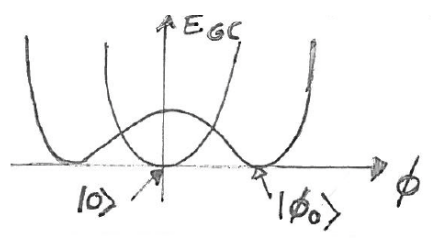
\includegraphics[width=0.4\linewidth]{Immagini - Capitolo 1/stati coerenti.png}
    \caption{stato di vuoto e stato coerente come stato di minima energia nella fase a simmetria rotta.}
    \label{fig: stati coerenti}
\end{figure}

\section{Approssimazione di Bogoljubov}
Si comincia separando la parte corrispondente allo stato fondamentale $\ko$ contenente gli operatori $\hata_0$ e $\hataT_0$ da quella relativa agli stati con $\vk \neq \vo$ considerandone solamente i termini quadratici in $\hata_k$, quindi l'hamiltoninana di partenza è
\begin{equation}
\label{eq: hamiltoniana G-P per approx. Bogoljubov}
    \begin{split}
        \hatH_{GP} &= \nsum_k\frac{\hbar^2k^2}{2m}\hataT_k\hata_k + \frac{g}{2V}\hataT_0\hataT_0\hata_0\hata_0 \\
        &+ \frac{g}{2V}\sum_{\vk \neq \vo}(4\hataT_0\hataT_k\hata_0\hata_k + \hataT_k\hataT_{-k}\hata_0\hata_0 + \hataT_0\hataT_0\hata_{-k}\hata_k) + o[(\hata_k)^3].
    \end{split}
\end{equation}
Infatti, nel termine $\sum_{k_1,k_2,q}\hataT_{k_2 + q}\hataT_{k_1 - q}\hata_{k_2}\hata_{k_1}$ ci sono sei termini che dipendono da due operatori $\hata_0$:
\begin{enumerate}
    \item $\hataT_q\hataT_{-q}\hata_0\hata_0$ per $(\vk_1 = \vo, \vk_2 = \vo)$;
    \item $\hataT_{k_2}\hataT_0\hata_{k_2}\hata_0$ per $(\vk_1 = \vo, \vk_1 - \vq = \vo)$;
    \item $\hataT_0\hataT_{k_2}\hata_{k_2}\hata_0$ per $(\vk_1 = \vo, \vk_2 + \vq = \vo)$;
    \item $\hataT_{k_1}\hataT_0\hata_0\hata_{k_1}$ per $(\vk_2 = \vo, \vk_1 - \vq = \vo)$;
    \item $\hataT_0\hataT_{k_1}\hata_0\hata_{k_1}$ per $(\vk_2 = \vo, \vk_2 + \vq = \vo)$;
    \item $\hataT_0\hataT_0\hata_{-k_1}\hata_{k_1}$ per $(\vk_1 - \vq = \vo, \vk_2 + \vq = \vo)$.
\end{enumerate}
Di questi sei termini $\hataT_q\hataT_{-q}\hata_0\hata_0$ e $\hataT_0\hataT_0\hata_{-k_1}\hata_{k_1}$ sono distinti, mentre gli altri quattro sono equivalenti a meno di rinominare le variabili, per cui 
\begin{equation}
    \hataT_{k_2}\hataT_0\hata_{k_2}\hata_0 + \hataT_0\hataT_{k_2}\hata_{k_2}\hata_0 + \hataT_{k_1}\hataT_0\hata_0\hata_{k_1} + \hataT_0\hataT_{k_1}\hata_0\hata_{k_1} = 4\hataT_0\hataT_k\hata_0\hata_k.
\end{equation}
Questi tre termini possono poi essere rappresentati graficamente come mostrato in figura \ref{fig: scattering 1, 2, 3}, interpretandoli come: lo scattering elastico tra una particella con $\vk \neq \vo$ e una del condensato; due particelle con impulso $\vk$ e $-\vk$ che escono dal condensato; due particelle con impulso $\vk$ e $-\vk$ che entrano nel condensato. In particolare, gli ultimi due processi non comportano una violazione della conservazione dell'energia in quanto le onde piane, ossia le particelle libere, non sono autofunzioni di $\hatH_{GP}$.
\begin{figure}[h]
    \centering
    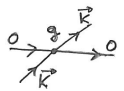
\includegraphics[width=0.2\linewidth]{Immagini - Capitolo 1/scattering 1.png}
    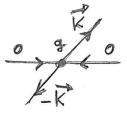
\includegraphics[width=0.2\linewidth]{Immagini - Capitolo 1/scattering 2.png}
    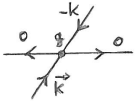
\includegraphics[width=0.2\linewidth]{Immagini - Capitolo 1/scattering 3.png}
    \caption{i termini di scattering distinti dell'hamiltoniana $\hatH_{GP}$ sono: (i) $\hataT_0\hataT_k\hata_0\hata_k$; (ii) $\hataT_k\hataT_{-k}\hata_0\hata_0$; (iii) $\hataT_0\hataT_0\hata_{-k}\hata_k$.}
    \label{fig: scattering 1, 2, 3}
\end{figure}

Si supponga ora che lo stato con $\vk = \vo$, su cui agiscono gli operatori $\hataT_0$ e $\hata_0$, sia uno stato coerente occupato in media dalla quasi totalità delle particelle, ossia $\hatN_0 \simeq \hatN$; per cui da
\begin{equation}
    \hatN = \hataT_0\hata_0 + \sum_{\vk \neq \vo}\hataT_k\hata_k = \hatN_0 + \sum_{\vk \neq \vo}\hataT_k\hata_k,
\end{equation}
si scrive il numero di particelle nello stato fondamentale in funzione di $\hatN$ invertendo la relazione
\begin{equation}
    \hatN_0 = \hatN - \sum_{\vk \neq \vo}\hataT_k\hata_k,
\end{equation}
considerando il termine $\sum_{\vk \neq \vo}\hataT_k\hata_k$ come una correzione al primo ordine dell'ordine zero $\hatN$. Si può allora scrivere il secondo termine dell'hamiltoniana \eqref{eq: hamiltoniana G-P per approx. Bogoljubov} come
\begin{equation}
    \begin{split}
        \frac{g}{2V}(\hataT_0\hataT_0\hata_0\hata_0) &= \frac{g}{2V}(\hatN^2 - 2\hatN\sum_{\vk \neq \vo}\hataT_k\hata_k) + \cdots \\
        &\simeq \frac{g}{2V}(N^2 - 2N\sum_{\vk \neq \vo}\hataT_k\hata_k),
    \end{split}
\end{equation}
dove si è sostituito a $\hatN$ il suo valore medio $\vmedio{\hatN} \equiv N$; l'hamiltoniana in questione quindi diventa l'hamiltoniana di Bogoljubov
\begin{equation}
\label{eq: hamiltoniana di Bogoljubov}
    \begin{split}
        \hatH_{GP} &\simeq \frac{gN^2}{2V} + \sum_{\vk \neq \vo}\frac{\hbar^2k^2}{2m}\hataT_k\hata_k - \frac{2gN}{2V}\sum_{\vk \neq \vo}\hataT_k\hata_k \\
        &+ \frac{g}{2V}\sum_{\vk \neq \vo}(4\hataT_0\hataT_k\hata_0\hata_k + \hataT_k\hataT_{-k}\hata_0\hata_0 + \hataT_0\hataT_0\hata_{-k}\hata_k) \\
        &= \frac{gN^2}{2V} + \sum_{\vk \neq \vo}\bigg(\frac{\hbar^2k^2}{2m} + \frac{2gN}{V}\bigg)\hataT_k\hata_k + \frac{gN}{2V}\sum_{\vk \neq \vo}(\hataT_k\hataT_{-k} + \hata_{-k}\hata_k) \\
        &\equiv \hatH_B
    \end{split}
\end{equation}
L'hamiltoniana $\hatH_B$ trovata può essere diagonalizzata attraverso la trasformazione di Bogoljubov.

\subsection{Trasformazione di Bogoljubov}
Prima di diagonalizzare direttamente $\hatH_B$, si considera un'hamiltoniana generica della forma
\begin{equation}
\label{eq: hamiltoniana generica h}
    \hath = \bar{\epsilon}(\hataT_1\hata_1 + \hataT_2\hata_2) + \lambda(\hataT_1\hataT_2 + \hata_2\hata_1),
\end{equation}
dove il secondo termine corrisponde ad un termine di interazione in quanto ``mescola'' gli operatori con indici diversi. Ad ogni modo, l'hamiltoniana $\hath$ può essere diagonalizzata utilizzando la trasformazione di Bogoljubov nel modo seguente. Si introducono due coppie di operatori di distruzione e creazione $(\hatd_1, \hatdT_1)$ e $(\hatd_2, \hatdT_2)$, legati agli operatori $(\hata_1, \hataT_1)$ e $(\hata_2, \hataT_2)$ attraverso la trasformazione canonica $\comm{\hatd_1}{\hatdT_1} = \comm{\hatd_2}{\hatdT_2} = 1$; si definisce la trasformazione di Bogoljubov
\begin{equation}
    \begin{cases}
        \hata_1 = u\hatd_1 + v\hatdT_2 \\
        \hataT_1 = u\hatdT_1 + v\hatd_2 \\
    \end{cases},\quad 
    \begin{cases}
        \hata_2 = u\hatd_2 + v\hatdT_1 \\
        \hataT_2 = u\hatdT_2 + v\hatd_1 \\
    \end{cases},\quad u,v \in \R,
\end{equation}
che infatti soddisfano le relazioni di commutazione
\begin{align}
    \begin{split}
        \comm{\hata_1}{\hataT_1} = \comm{u\hatd_1 + v\hatdT_2}{u\hatdT_1 + v\hatd_2} &= u\comm{\hatd_1}{u\hatdT_1 + v\hatd_2} + v\comm{\hatdT_2}{u\hatdT_1 + v\hatd_2} \\
        &= u^2\comm{\hatd_1}{\hatdT_1} + v^2\comm{\hatdT_2}{\hatd_2} \\
        &= u^2 - v^2 \\
        &= 1,
    \end{split} \\
    \begin{split}
        \comm{\hata_2}{\hataT_2} = \comm{u\hatd_2 + v\hatdT_1}{u\hatdT_2 + v\hatd_1} &= u\comm{\hatd_2}{u\hatdT_2 + v\hatd_1} + v\comm{\hatdT_1}{u\hatdT_2 + v\hatd_1} \\
        &= u^2\comm{\hatd_2}{\hatdT_2} + v^2\comm{\hatdT_1}{\hatd_1} \\
        &= u^2 - v^2 \\
        &= 1.
    \end{split}
\end{align}
Da queste ultime due relazioni si può pensare di parametrizzare i coefficienti $u$ e $v$ come $u = \cosh{\alpha}$ e $v = \sinh{\alpha}$, dove $\alpha$ deve essere fissato in modo da diagolinazzare $\hath$, così da poter usare anche le proprietà trigonometriche $u^2 + v^2 = \cosh{(2\alpha)}$ e $2uv = \sinh{(2\alpha)}$. Adesso, si riscrive $\hath$ in forma matriciale
\begin{equation}
\label{eq: hamiltoniana generica h in forma matriciale}
    \hath = \frac{1}{2}
    \begin{pmatrix}
        \hataT_1 & \hata_2 & \hataT_2 & \hata_1
    \end{pmatrix}
    \begin{pmatrix}
        \bar{\epsilon} & \lambda & 0 & 0 \\
        \lambda & \bar{\epsilon} & 0 & 0 \\
        0 & 0 & \bar{\epsilon} & \lambda \\
        0 & 0 & \lambda & \bar{\epsilon}
    \end{pmatrix}
    \begin{pmatrix}
        \hata_1 \\
        \hataT_2 \\
        \hata_2 \\
        \hataT_1
    \end{pmatrix} - \bar{\epsilon}
\end{equation}
\begin{obs}
    Si può verificare che effettivamente la riscrittura \eqref{eq: hamiltoniana generica h in forma matriciale} dell'hamiltoniana \eqref{eq: hamiltoniana generica h} considerando che la parte diagonale è
    \begin{equation}
        \begin{split}
            \frac{1}{2}
            \begin{pmatrix}
            \hataT_1 & \hata_2 & \hataT_2 & \hata_1
        \end{pmatrix}
        \begin{pmatrix}
            \hata_1 \\
            \hataT_2 \\
            \hata_2 \\
            \hataT_1
        \end{pmatrix} &= \frac{1}{2}\bar{\epsilon}(\hataT_1\hata_1 + \hata_2\hataT_2 + \hataT_2\hata_2 + \hata_1\hataT_1) \\
        &= \bar{\epsilon}(\hataT_1\hata_1 + \hataT_2\hata_2) + \bar{\epsilon},
        \end{split}
    \end{equation}
    mentre la parte non diagonale restituisce per il primo blocco
    \begin{equation}
        \frac{1}{2}
            \begin{pmatrix}
                \hataT_1 & \hata_2
            \end{pmatrix}
            \begin{pmatrix}
                0 & \lambda \\
                \lambda & 0
            \end{pmatrix}
            \begin{pmatrix}
                \hata_1 \\
                \hataT_2
            \end{pmatrix} = \frac{\lambda}{2}(\hataT_1\hataT_2 + \hata_2\hata_1),
    \end{equation}
    e per il secondo blocco un risultato analogo semplicemente scambiando gli indici $1$ e $2$; mettendo tutto insieme si ottiene proprio l'espressione \eqref{eq: hamiltoniana generica h}.
\end{obs}
Si parte dal primo blocco della matrice diagonale
\begin{equation}
    \begin{pmatrix}
        \hataT_1 & \hata_2
    \end{pmatrix}
    \begin{pmatrix}
        \bar{\epsilon} & \lambda \\
        \lambda & \bar{\epsilon}
    \end{pmatrix}
    \begin{pmatrix}
        \hata_1 \\
        \hataT_2
    \end{pmatrix}
\end{equation}
da cui, sostituendo la trasformazione di Bogoljubov definita dalle espressioni
\begin{equation}
    \begin{pmatrix}
        \hata_1 \\
        \hataT_2
    \end{pmatrix} = 
    \begin{pmatrix}
        u & v \\
        v & u
    \end{pmatrix}
    \begin{pmatrix}
        \hatd_1 \\
        \hatdT_2
    \end{pmatrix}, \quad 
    \begin{pmatrix}
        \hataT_1 & \hata_2
    \end{pmatrix} = 
    \begin{pmatrix}
        \hatdT_1 & \hatd_2
    \end{pmatrix}
    \begin{pmatrix}
        u & v \\
        v & u
    \end{pmatrix},
\end{equation}
si trova che
\begin{multline}
    \begin{pmatrix}
        \hatdT_1 & \hatd_2
    \end{pmatrix}
    \begin{pmatrix}
        u & v \\
        v & u
    \end{pmatrix}
    \begin{pmatrix}
        \bar{\epsilon}u + \lambda v & \bar{\epsilon}v + \lambda u \\
        \bar{\epsilon}v + \lambda u & \bar{\epsilon}u + \lambda v
    \end{pmatrix}
    \begin{pmatrix}
        \hatd_1 \\
        \hatdT_2
    \end{pmatrix} = \\
    = \begin{pmatrix}
        \hatdT_1 & \hatd_2
    \end{pmatrix}
    \begin{pmatrix}
        \bar{\epsilon}(u^2 + v^2) + 2\lambda uv & 2\bar{\epsilon} uv + \lambda(u^2 + v^2) \\
        2\bar{\epsilon} uv + \lambda(u^2 + v^2) & \bar{\epsilon}(u^2 + v^2) + 2\lambda uv 
    \end{pmatrix}
    \begin{pmatrix}
        \hatd_1 \\
        \hatdT_2
    \end{pmatrix}.
\end{multline}
Adesso, imponendo che i termini fuori dalla diagonale si annullino con $\bar{\epsilon} uv + \lambda(u^2 + v^2) = 0$, usando la parametrizzazione dei coefficienti $u$ e $v$ insieme alle loro proprietà, si trova che 
\begin{equation}
    \lambda = -\bar{\epsilon}\tanh{(2\alpha)};
\end{equation}
di conseguenza, i termini sulla diagonale diventano
\begin{equation}
    \bar{\epsilon}\cosh{(2\alpha)} - \bar{\epsilon}\frac{\sinh^2{(2\alpha)}}{\cosh{(2\alpha)}} = \frac{\bar{\epsilon}}{\cosh{(2\alpha)}} = \bar{\epsilon}\sqrt{1 - \tanh^2{(2\alpha)}} = \bar{\epsilon}\sqrt{1 - \frac{\lambda^2}{\bar{\epsilon}^2}},
\end{equation}
dove si è considerata la radice quadrata positiva in quanto $\bar{\epsilon}/\cosh{(2\alpha)}$ è una quantità positiva. Quindi, si arriva all'espressione
\begin{equation}
    \begin{pmatrix}
        \hatdT_1 & \hatd_2
    \end{pmatrix}
    \begin{pmatrix}
        \sqrt{\bar{\epsilon}^2 - \lambda^2} & 0 \\
        0 & \sqrt{\bar{\epsilon}^2 - \lambda^2}
    \end{pmatrix}
    \begin{pmatrix}
        \hatd_1 \\
        \hatdT_2
    \end{pmatrix} \equiv 
    \begin{pmatrix}
        \hatdT_1 & \hatd_2
    \end{pmatrix}
    \begin{pmatrix}
        \epsilon & 0 \\
        0 & \epsilon
    \end{pmatrix}
    \begin{pmatrix}
        \hatd_1 \\
        \hatdT_2
    \end{pmatrix},
\end{equation}
dove si è posto $\epsilon \equiv \sqrt{\bar{\epsilon}^2 - \lambda^2}$. Analogamente, con procedimenti simili si arriva al medesimo risultato per il secondo blocco della matrice dato che è identico al primo. Dunque, l'hamiltoniana diagonalizzata è
\begin{equation}
    \begin{split}
        \hath &= \frac{1}{2}
        \begin{pmatrix}
            \hatdT_1 & \hatd_2 & \hatdT_2 & \hatd_1
        \end{pmatrix}
        \diag{\epsilon, \epsilon, \epsilon, \epsilon}
        \begin{pmatrix}
            \hatd_1 \\
            \hatdT_2 \\
            \hatd_2 \\
            \hatdT_1
        \end{pmatrix}
        - \bar{\epsilon} \\
        &= \frac{\epsilon}{2}(\hatdT_1\hatd_1 + \hatd_2\hatdT_2 + \hatdT_2\hatd_2 + \hatd_1\hatdT_1) - \bar{\epsilon} \\
        &= \epsilon(\hatdT_1\hatd_1 + \hatdT_2\hatd_2) + (\epsilon - \bar{\epsilon}).
    \end{split}
\end{equation}
Adesso si hanno tutti gli strumenti per diagonalizzare $\hatH_B$, che quindi diventa
\begin{equation}
    \begin{split}
        \hatH_B &= \frac{gN^2}{2V} + \sum_{\vk \neq \vo}\bigg(\frac{\hbar^2k^2}{2m} + \frac{gN}{V}\bigg)\hataT_k\hata_k + \frac{gN}{V}\sum_{\vk \neq \vo}(\hataT_k\hataT_{-k} + \hata_{-k}\hata_k) \\
        &= \frac{gN^2}{2V} + \frac{1}{2}\sum_{\vk \neq \vo}\bigg[\bar{\epsilon}(\hataT_k\hata_k + \hataT_{-k}\hata_{-k}) + \lambda(\hataT_k\hataT_{-k} + \hata_{-k}\hata_k)\bigg],
    \end{split}
\end{equation}
dove si sono posti
\begin{equation}
    \bar{\epsilon}(k) = \frac{\hbar^2k^2}{2m} + \frac{gN}{V},\quad \lambda = \frac{gN}{V} \equiv \mu.
\end{equation}
Il risultato della trasformazione di Bogoljubov è
\begin{equation}
    \epsilon(k) = \sqrt{\bar{\epsilon}(k)^2 - \lambda^2},
\end{equation}
da cui, sostituendo le relazioni precedenti, si ricava la legge di dispersione di Bogoljubov
\begin{equation}
\label{eq: legge di dispersione di Bogoljubov}
    \epsilon(k) = \sqrt{\epsilon_0(k)^2 + 2\mu\epsilon_0(k)},
\end{equation}
la stessa già trovata nell'equazione \eqref{eq: relazione di dispersione di Bogoljubov}. Se si sostituisce nell'hamiltoniana \eqref{eq: hamiltoniana di Bogoljubov} la legge di dispersione \eqref{eq: legge di dispersione di Bogoljubov} si trova
\begin{equation}
    \hatH_B = E_0 + \sum_{\vk \neq \vo}\epsilon(k)\hatdT_k\hatd_k,\quad E_0 = \frac{gN^2}{2V} + \frac{1}{2}\sum_{\vk \neq \vo}[\epsilon(k) - \bar{\epsilon}(k)].
\end{equation}
Quest'ultimo risultato implica che il sistema originario composto da particelle interagenti può essere descritto da un'hamiltoniana di quasi-particelle libere con legge di dispersione data da \eqref{eq: legge di dispersione di Bogoljubov}. Ci si domanda in ultima istanza se è possibile trovare un'espressione dei coefficienti $u$ e $v$ in funzione di $\vk$. Si parte quindi dal sistema 
\begin{equation}
    \begin{cases}
        u^2 - v^2 = 1 \\
        2\bar{\epsilon}uv + \lambda(u^2 + v^2) = 0
    \end{cases};
\end{equation}
la prima equazione è soddisfatta dalla parametrizzazione 
\begin{equation}
\label{eq: parametrizzazione coefficienti u e v}
    \begin{cases}
        u^2 = \dfrac{\gamma}{2} + \dfrac{1}{2} \\[2ex]
        v^2 = \dfrac{\gamma}{2} - \dfrac{1}{2}
    \end{cases},
\end{equation}
che sostituita nella seconda equazione del sistema restituisce
\begin{equation}
    \begin{split}
        2\bar{\epsilon}\sqrt{\frac{\gamma^2}{4} - \frac{1}{4}} &= -\lambda\bigg(\frac{\gamma}{2} + \frac{1}{2} + \frac{\gamma}{2} - \frac{1}{2}\bigg) \\
        \bar{\epsilon}\sqrt{\gamma^2 - 1} &= -\lambda\gamma \\
        \bar{\epsilon}^2(\gamma^2 - 1) &= \lambda^2\gamma^2,
    \end{split}
\end{equation}
da cui si ha 
\begin{equation}
    \gamma = \frac{\bar{\epsilon}}{\sqrt{\bar{\epsilon}^2 - \lambda^2}} > 1.
\end{equation}
Dunque, sostituendo l'espressione trovata per $\gamma$ nella parametrizzazione \eqref{eq: parametrizzazione coefficienti u e v} si trovano
\begin{equation}
    u_k = \sqrt{\frac{\bar{\epsilon}}{2\sqrt{\bar{\epsilon}^2 - \lambda^2}} + \frac{1}{2}},\quad v_k = -\sqrt{\frac{\bar{\epsilon}}{2\sqrt{\bar{\epsilon}^2 - \lambda^2}} - \frac{1}{2}}.
\end{equation}
Si considerano infine due limiti particolari:
\begin{enumerate}
    \item se $g \simeq 0$ e $\vk$ è una quantità finita, allora si ha che 
    \begin{equation}
        \epsilon \simeq \bar{\epsilon} \simeq \frac{\hbar^2k^2}{2m},\quad \lambda \simeq 0,
    \end{equation}
    e poiché $\hataT_k = u_k\hatdT_k + v_k\hatd_k$, in questo limite, dato che $u_k \simeq 1$ e $v_k \simeq 0$, si ha che $\hataT_k \simeq \hatdT_k$, la quale identifica il limite di particella libera;
    \item se $g$ è una quantità finita e $\vk \simeq 0$, allora si ha che
    \begin{equation}
        \bar{\epsilon}(k) \simeq \frac{gN}{V} \equiv \mu,\quad \epsilon(k) \simeq v_1\hbar k,
    \end{equation}
    i coefficienti sono legati dalla relazione
    \begin{equation}
        u_k \simeq \sqrt{\frac{\mu}{2v_1\hbar k}} \simeq \frac{1}{\sqrt{k}}\sqrt{\frac{\mu}{2v_1\hbar}} \simeq -v_k,
    \end{equation}
    mentre per gli operatori si ha
    \begin{equation}
        \hataT_k \simeq \frac{1}{\sqrt{k}}(\hatdT_k - \hatd_{-k})\sqrt{\frac{\mu}{2v_1\hbar}},
    \end{equation}
    che implica l'evoluzione temporale dell'operatore
    \begin{equation}
        \hataT_k(t) \simeq \frac{1}{\sqrt{k}}(\hatdT_ke^{i\epsilon t/\hbar} - \hatd_{-k}e^{-i\epsilon t/\hbar})\sqrt{\frac{\mu}{2v_1\hbar}},
    \end{equation}
    da quest'ultimo risultato si deduce che una particella ``reale'' a piccoli valori di $\vk$ corrisponde ad oscillazioni di densità di fononi.
\end{enumerate}

\section{Deplezione quantistica}
Lo stato vuoto, per la teoria di un gas di bosoni interagenti con potenziale a delta di Dirac, nell'approssimazione di Bogoliubov è definito da $\hatd_k\ket{B} = 0$, per ogni $k$, cioè lo stato di vuoto è caratterizzato dall'assenza totale di quasi-particelle. Tuttavia, ci si domanda se si può affermare che $\ket{B}$ sia composto solo da particelle di massa $m$ nello stato con energia cinetica e momento nulli, in altre parole, vale che $\hata_k\ket{B} = 0$ per ogni $k$?. Per capirlo, si definisce l'operatore numero di pseudo-particelle con impulso $\vk$ come
\begin{equation}
    \hatN_k^B := \hatdT_k\hatd_k,
\end{equation}
dove essendo le particelle dei bosoni $\comm{\hatdT_k}{\hatdT_{k'}} = 0$ e a temperatura $T \neq \SI{0}{\kelvin}$ si ha
\begin{equation}
    N_k^B \equiv \vmedio{N_k^B}_T = \vmedio{\hatdT_k\hatd_k}_T = \frac{1}{e^{\beta\epsilon(k)} - 1},
\end{equation}
il quale non ha nulla a che fare con il numero medio di particelle ``reali'' di massa $m$ che compongono il gas. Usando la trasformazione di Bogoliubov
\begin{equation}
    \begin{cases}
        \hata_k = u_k\hatd_k + v_k\hatdT_{-k} \\
        \hataT_k = u_k\hatdT_k + v_k\hatd_{-k}
    \end{cases},
\end{equation}
si calcola
\begin{equation}
    \begin{split}
        N_k &= \vmedio{(u_k\hatdT_k + v_k\hatd_{-k})(u_k\hatd_k + v_k\hatdT_{-k})} \\
        &= u_k^2\vmedio{\hatdT_k\hatd_k} + v_k^2\vmedio{\hatd_{-k}\hatdT_{-k}}_T + u_kv_k\vmedio{\hatdT_k\hatdT_{-k}}_T + v_ku_k\vmedio{\hatd_k\hatd_k} \\
        &= u_k^2\vmedio{\hatdT_k\hatd_k}_T + v_k^2\vmedio{\hatdT_{-k}\hatd_{-k}}_T + v_k^2 \\
        &= (u_k^2 + v_k^2)\vmedio{\hatdT_k\hatd_k}_T + v_k^2 \\
        &= (u_k^2 + v_k^2)N_k^B + v_k^2,
    \end{split}
\end{equation}
dove si è sfruttata la simmetria $k \longleftrightarrow -k$ e posto $\vmedio{\hatdT_k\hatd_k}_T = \vmedio{\hatdT_{-k}\hatd_{-k}}_T$ e $\vmedio{\hatd_k\hatd_{-k}}_T = \vmedio{\hatdT_k\hatdT_{-k}}_T = \vmedio{\hatd_k}_T\vmedio{\hatd_{-k}}_T = 0$ per uno stato all'equilibrio termico. Per determinare quante particelle occupano lo stato con $\vk = \vo$, si considera che
\begin{equation}
    \hatN_0 = \hatN - \sum_{k \neq 0}\hatN_k,
\end{equation}
da cui, passando al continuo, si calcola il valore medio
\begin{equation}
    \begin{split}
        N_0 &= N - \frac{V}{h^3}\int d^3k\,\bigg[v^2_k + \frac{v^2_k + u^2_k}{e^{\beta\epsilon(k)} - 1}\bigg] \\
        &= N - \frac{V}{h^3}\int d^3k\,v^2_k - \frac{V}{h^3}\int d^3k\,\frac{v^2_k + u^2_k}{e^{\beta\epsilon(k)} - 1},
    \end{split} 
\end{equation}
dove il secondo termine corrisponde alla deplezione quantistica, mentre il terzo alla deplezione termica. Infatti, il terzo termine a $T = \SI{0}{\kelvin}$ si annulla e rimane solamente il termine quantistico
\begin{equation}
    N_0(T = 0) = N - \frac{V}{h^3}\int d^3k\,v^2_k.
\end{equation}
Pertanto, una frazione finita di particelle del gas si trova in uno stato con $\vk \neq \vo$ e non fa quindi parte del condensato sebbene non vi siano pseudo-particelle e tutto il gas sia superfluido. L'effetto di deplezione quantistica svanisce nel limite $g \to 0$. In particolare, nell'elio-II la percentuale di particelle nello stato $\vk = \vo$ misurata sperimentalmente è circa solo l'8\%. Nonostante questo, la componente normale dell'elio-II è nulla a $T = \SI{0}{\kelvin}$. Nei moderni esperimenti con gas rarefatti a bassa temperatura si arriva a percentuali prossime al 100\%. Tuttavia, va notato che i gas reali diluiti a bassa temperatura sono metastabili: il vero stato fondamentale è solido. Nonostante questo, lo stato metastabile sopravvive per tempi sufficientemente lunghi da permettere la raccolta di tutti i dati sperimentali di interesse fisico. D'altra parte, a temperature più alte, il termine ``classico'' diventa dominante. Quindi, negli esperimenti bisogna operare a bassa temperatura per evitare la deplezione termica e con gas rarefatti per diminuire il valore efficace della costante $g$ e ridurre al minimo la deplezione quantistica. 

% \chapter{Superconduttività}
La superconduttività fu scoperta per la prima volta nel 1911 da Kamerlingh Onnes durante uno studio riguardante la resistività dei metalli puri a bassa temperatura. Onnes osservò che la resistività del campione di mercurio oggetto di studio scendeva drasticamente a temperature sotto i $\SI{4.2}{\kelvin}$, come mostrato in figura \ref{fig: resistività Hg}. 
\begin{figure}[h]
    \centering
    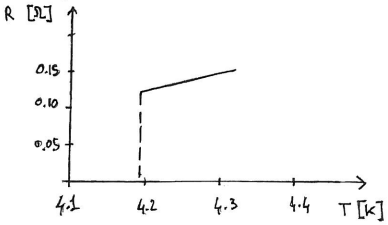
\includegraphics[width=0.5\linewidth]{Immagini - Capitolo 2/resistività Hg.png}
    \caption{andamento della resistenza $R$ del mercurio in funzione della temperatura.}
    \label{fig: resistività Hg}
\end{figure}

Valori di resistenza anche molto piccoli possono essere misurati attraverso la diminuzione della corrente in un conduttore ad anello. La corrente in quest'ultimo dovrebbe diminuire secondo la legge 
\begin{equation}
    i(t) = I_0e^{-Rt/L},
\end{equation}
dove $L$ è l'induttanza dell'anello. Dagli esperimenti di questo tipo si può concludere che la resistività crolla di almeno sedici ordini di grandezza scendendo al di sotto di una certa temperatura critica $T_c$, entrando nel regime di superconduzione. In queste condizioni la corrente scorre senza subire fenomeni di dissipazione dimostrando che la resistività di un superconduttore non è solo piccola ma essenzialmente nulla. La temperatura critica, o di transizione, dipende quasi esclusivamente dalla natura del superconduttore e varia in un range molto ampio, alcuni esempi sono elencati in tabella \ref{tab: esempi di temperature critiche}.
\begin{table}[h]
    \centering
    \begin{tabular}{|c|c|}
        \hline
         Elemento & $T_c\,[\mathrm{K}]$ \\ \hline
         $\ce{Al}$ & 1.19 \\
         $\ce{Hg}$ & 4.15 \\ 
         $\ce{Ga}$ & 1.09 \\ 
         $\ce{HgBa2Ca2Cu3O_x}$ & 135 \\ \hline
    \end{tabular}
    \caption{esempi di temperature critiche di alcuni elementi.}
    \label{tab: esempi di temperature critiche}
\end{table}
Infatti, la struttura reticolare non è rilevante per determinare quali materiali possono essere superconduttori: cristalli puri, leghe e metalli amorfi possiedono proprietà di superconduzione; persino il silicio diventa un superconduttore, seppur ad alta pressione e bassa temperatura. Tipicamente, i metalli puri entrano in regime di conduzione al di sotto dei $\SI{10}{\kelvin}$, mentre i composti metallici attorno ai $\SI{20}{\kelvin}$. Ottimi conduttori come l'oro, il rame e l'argento non entrano in regime di conduttore fino a temperature nell'ordine del kelvin. In generale, nemmeno le impurità influiscono sul comportamento di un superconduttore, a parte le impurità magnetiche. Queste ultime infatti tendono ad intrappolare elettroni e ad annullare le proprietà di superconduttività, un fenomeno che prende il nome di effetto Kondo. Tipicamente, la transizione di fase a supeconduttore avviene senza un cambiamento della struttura reticolare. Inoltre, materiali composti possono essere superconduttori sebbene i loro singoli costituenti rimangano nel regime di conduzione normale. Risulta invece essere rilevante il volume atomico, infatti normalmente materiali composti da volumi atomici grandi sono sfavoriti ad entrare in superconduzione. 

\section{Effetto Meissner-Ochsenfeld}
Nel 1933, Meissner e Ochsenfeld scoprirono che la transizione al regime di superconduzione non corrisponde solo alla quasi totale assenza di resistenza, ma anche alla comparsa di un comportamento diamagnetico ideale. Questo effetto sta anche alla base della distinzione tra un superconduttore e un conduttore ideale con resistenza nulla. Dalla legge di Faraday
\begin{equation}
    \frac{\p \Phi(t)}{\p t} = -\oint_{\p\Sigma}\vE \cdot d\bm{\Sigma},
\end{equation}
si ha che la variazione di flusso di campo magnetico attraverso un cammino chiuso induce un campo elettrico $\vE$. Tuttavia, in un conduttore ideale e in un superconduttore la resistenza è nulla, per cui non vi possono essere differenze di potenziale, quindi un campo elettrico, per cui il campo magnetico $\vB$ risulta stazionario all'interno di essi. Nella pratica, la schermatura del campo magnetico esterno avviene grazie alla formazioni di correnti superficiali di superconduzione.

Si considerino quindi due esperimenti in cui si confronta il comportamento di un conduttore ideale con quello di un superconduttore. Dato un campo magnetico esterno $\vB_a$, si indica con $t_0$ l'istante in cui viene raggiunto il regime di superconduzione. Nel primo esperimento, mostrato sempre in figura \ref{fig: effetto M-O I e II}, per entrambi i campioni il campo magnetico non può penetrare al loro interno. Dato che la resistenza è nulla, la corrente schermante in entrambi i casi non si dissipa fino alla scomparsa del campo magnetico esterno. Nel secondo esperimento, mostrato in figura \ref{fig: effetto M-O I e II}, il campo magnetico viene acceso prima dell'istante $t_0$, il quale non viene schermato da entrambi i campioni. Tuttavia, dopo l'istante $t_0$, il campo magnetico viene schermato solo dal superconduttore, mentre il conduttore ideale continua ad essere attraversato da esso. Quando poi il campo magnetico viene spento, il conduttore ideale rimane magnetizzato, mentre il superconduttore non presenta alcun segno della presenza di $\vB_a$. Questa differenza nel comportamento dei due campioni è proprio l'effetto di Meissner-Ochsenfeld. 
\begin{figure}[h]
    \centering
    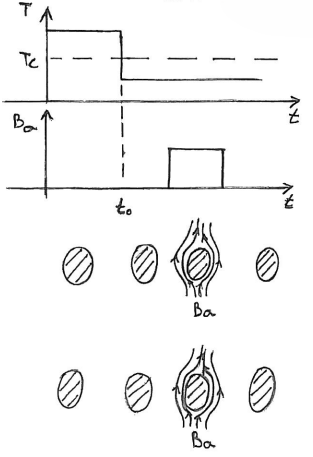
\includegraphics[width=0.4\linewidth]{Immagini - Capitolo 2/effetto M-O I.png}
    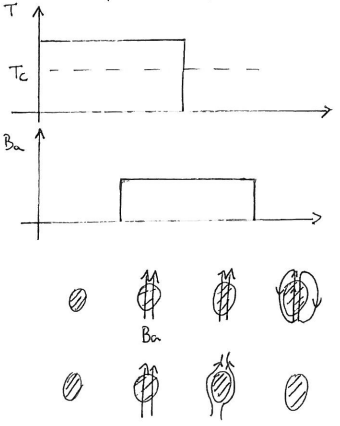
\includegraphics[width=0.45\linewidth]{Immagini - Capitolo 2/effetto M-O II.png}
    \caption{visualizzazione dell'effetto Meissner-Ochsenfeld (la prima riga si riferisce al conduttore ideale, la seconda al superconduttore).}
    \label{fig: effetto M-O I e II}
\end{figure}

Nel caso di un conduttore ad anello, la situazione non è molto differente. Il campo magnetico viene espulso dall'interno del superconduttore, ma si instaurano delle correnti schermanti sulla superficie che persistono anche quando il campo magnetico cessa di esserci, come mostrato in figura \ref{fig: effetto M-O III}. Si noti comunque come il flusso di campo magnetico all'interno dell'anello non viene respinto dal superconduttore.
\begin{figure}[h]
    \centering
    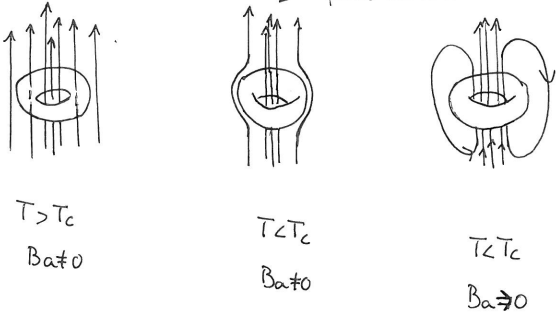
\includegraphics[width=0.5\linewidth]{Immagini - Capitolo 2/effetto M-O III.png}
    \caption{effetto Meissner-Ochsenfeld in un superconduttore ad anello.}
    \label{fig: effetto M-O III}
\end{figure}

Ad ogni modo, un forte campo magnetico esterno può distruggere la superconduttività, ristabilendo lo stato normale di conduzione. A seconda del tipo di transizione, si possono distinguere due tipi di superconduttori, quelli di tipo I e quelli di tipo II.

\section{Superconduttori di tipo I}
Il comportamento di un superconduttore di tipo I immerso in campo magnetico esterno $\vB_a$ è mostrato in figura \ref{fig: SC tipo I}, dove si osserva un valore critico $\vB_c$ del campo magnetico che sancisce il confine tra il regime di conduzione normale e quello di superconduzione. Il campo magnetico interno al superconduttore può essere scritto 
\begin{equation}
    B_i = B_a + \mu_0M = \mu_0(H_a + M),
\end{equation}
dove $\mu_0$ è il coefficiente di suscettività magnetica nel vuoto. Per temperature $T < T_c$ si ha che $B_i = 0$ se e solo se
\begin{equation}
    \chi = \mu_0\frac{\p M}{\p B_a}\bigg|_{B_a = 0} = \frac{\mu_0M}{B_a} = -1.
\end{equation}
Questo risultato esprime il fatto che i superconduttori di tipo I sono diamagneti ideali. Se il campo magnetico esterno viene incrementato, la schermatura si ``rompe'' al valore critico $B_c$ e il conduttore ritorna allo stato normale di conduzione. Il valore del campo magnetico critico dipende dalla temperatura del materiale, in particolare segue la legge empirica
\begin{equation}
\label{eq: valore cricito Bc nei SC di tipo I}
    B_c(T) = B_c(0)\bigg[1 - \bigg(\frac{T}{T_c}\bigg)^2\bigg].
\end{equation}
\begin{figure}[h]
    \centering
    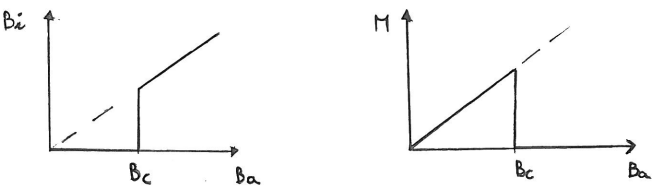
\includegraphics[width=0.7\linewidth]{Immagini - Capitolo 2/SC tipo I.png}
    \caption{andamento in funzione di $B_a$: (i) del campo magnetico interno al superconduttore $\vB_i$; (ii) della magnetizzazione $M$.}
    \label{fig: SC tipo I}
\end{figure}

Analogamente, quando un superconduttore è percorso da una corrente elettrica $I > I_c$, il campione transisce al regime normale. Per determinare il valore critico della corrente $I_c$ si deve considerare che in nessuna regione del superconduttore la corrente può superare $I_c$. Non ha importanza che questa sia la corrente di schermaggio o causata da un generatore di corrente ai capi del superconduttore. Si considera quindi un filo di raggio $R$, il campo magnetico sulla superficie del cavo è
\begin{equation}
    B = \frac{\mu_0I}{2\pi R},
\end{equation}
di conseguenza la corrente critica è semplicemente data da
\begin{equation}
    I_c = \frac{2\pi RB_c}{\mu_0},
\end{equation}
da cui si nota la proporzionalità con la circonferenza del filo, e non con la sua area. Alcuni esempi di superconduttori di tipo I sono il piombo, il mercurio e l'alluminio.

\section{Superconduttori di tipo II}
Come in quelli di tipo I, il campo magnetico viene completamente espulso fino a quando il valore del campo è inferiore ad un primo valore critico $B_{c_1}$. A valori superiori si formano canali di conduttore normale in regime di conduzione normale che permettono al campo esterno $\vB_a$ di penetrare nella forma di filamenti sottili, chiamati linee di flusso o vortici di superconduttori.
\begin{obs}
    Si vedrà che il flusso del campo magnetico, per ognuno di questi filamenti, o equivalentemente la circuitazione delle supercorrenti, non è quantizzata.
\end{obs}
L'esistenza di due tipi di superconduttore è legata all'energia di interfaccia tra regimi normale e di superconduzione che è positiva in quelli di tipo I, ma negativa in quelli di tipo II, favorendo così la formazione regioni di conduzione normale all'interno dei secondi. Il campo magnetico e la magnetizzazione all'interno di un superconduttore di tipo II, in funzione del campo magnetico applicato, hanno l'andamento la forma mostrata in figura \ref{fig: SC tipo II}.
\begin{figure}[h]
    \centering
    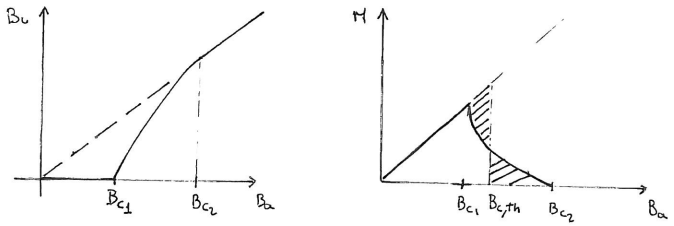
\includegraphics[width=0.7\linewidth]{Immagini - Capitolo 2/SC tipo II.png}
    \caption{andamento in funzione di $B_a$: (i) del campo magnetico interno al superconduttore $\vB_i$; (ii) della magnetizzazione $M$.}
    \label{fig: SC tipo II}
\end{figure}

Il secondo valore critico del campo magnetico $B_{c_2}$ in questo tipo di superconduttori può anche essere cento volte più alto del valore critico $B_c$ nei superconduttori di tipo I, risultando così più utili in applicazioni tecnologiche. I valori di $B_{c_1}$ e $B_{c_2}$ dipendono anch'essi dalla temperatura con un andamento parabolico simile a quello visto in equazione \eqref{eq: valore cricito Bc nei SC di tipo I}. In particolare, nei cristalli perfetti, le linee di flusso sono sistemate in modo regolare secondo il reticolo di Abrikosov, identico a quello osservato nei superfluidi in rotazione. 

\section{Termodinamica dei superconduttori}
La Termodinamica è basata sui principi generali e non dipende dalla descrizione microscopica del modello, essendo quindi in gradi di fornire risultati universali. Si considera il campo magnetico esterno $\vB \equiv \vB_a = \mu_0\vH$ come variabile indipendente e si descrive il sistema utilizzando l'insieme di variabili indipendenti $\{T,p,B\}$, ossia tramite l'energia libera di Gibbs 
\begin{equation}
    G = U - TS +pV - \vm \cdot \vB.
\end{equation}
Poiché $\vm$ e $\vB$ sono paralleli si possono ignorare le proprietà vettoriali e tenere conto solo del segno del momento magnetico. La variazione di energia libera quindi è 
\begin{equation}
    dG = -SdT + Vdp - mdB.
\end{equation}
Si vuole ora confrontare l'energia libera di Gibbs della fase normale con quella della fase superconduttiva.  Questa differenza è intimamente connessa con la natura della transizione di fase. Si supponga che il fattore di demagnetizzazione sia nullo e si trascurino i cambiamenti dovuti alla variazione di pressione. Per il superconduttore, si ha come magnetizzazione $M = m/V = -B/\mu_0$; per cui 
\begin{equation}
    dG_S  = -SdT + \cancelto{0}{Vdp} - mdB = -SdT + \frac{VB}{\mu_0}dB
\end{equation}
ed integrando
\begin{equation}
    G_S(B,T) = G_S(0,T) + \int_0^BdB'\,\frac{VB'}{\mu_0} = G_S(0,T) + \frac{VB^2}{2\mu_0},
\end{equation}
si trova un'espressione dove l'ultimo termine è positivo, indicando che l'energia necessaria per repellere il campo magnetico è positiva. Nel metallo normale, si trascurano le variazioni di energia dovute al campo magnetico poiché le variazioni di magnetizzazione dovute alla superconduttività sono molto più grandi rispetto al paramagnetismo o al diamagnetismo dei conduttori normali, per cui si ha $G_N(B,T) \simeq G_N(0,T)$. In accordo con
\begin{equation}
    G_S(B,T) = G_S(0,T) + \frac{VB^2}{2\mu_0},
\end{equation}
l'energia libera di Gibbs aumenta al crescere del campo magnetico: ad un certo punto necessariamente $G_S(B,T) \ge G_N(B,T)$ e lo stato superconduttore diventa instabile, ritornando allo stato normale. Quindi, deve esistere un valore di soglia $B_c$ tale per cui 
\begin{equation}
    G_S(B_c,T) = G_N(B_c,T) \simeq G_N(0,T) = G_S(0,T) + \frac{VB_c^2}{2\mu_0},
\end{equation}
da cui si ha
\begin{equation}
    G_N(0,T) - G_S(0,T) = \frac{V}{2\mu_0}B_c(T)^2,\quad B_C(T) \simeq B_c(0)\bigg(1 - \frac{T^2}{T_c^2}\bigg),
\end{equation}
dove poiché $G_N(B_c,T_c) = G_S(B_c,T_c)$, allora $B_c(T) \to 0$ per $T \to T_c$, come infatti mostra l'andamento di $B_c(T)$. Dalla differenza di energia libera tra il conduttore normale e il superconduttore, ricordando che $\p G/\p T = -S$, si può determinare la differenza di entropia come
\begin{equation}
    \Delta S= S_N(0,T) - S_S(0,T) = -\frac{VB_c}{\mu_0}\frac{dB_c(T)}{dT} \simeq \frac{2VB_c(0)^2}{\mu_0T_c^2}\bigg(1 - \frac{T^2}{T_c^2}\bigg)T.
\end{equation}
Per $T \to T_c$, la differenza di entropia $\Delta S$ tende ad annullarsi, come accade per il calore latente $\Delta Q = T_c\Delta S$; pertanto, la transizione è del secondo ordine, per $B = 0$. Analogamente, per $T \to 0$, ancora $\Delta Q \to 0$, ossia $\Delta S \to 0$, come ci si aspetta dal terzo principio della Termodinamica. Invece, per $0 < T < T_c$, si ha che
\begin{equation}
    \frac{dB_c(T)}{dT} <0, \quad \Delta S > 0,
\end{equation}
ossia il superconduttore è più ordinato del conduttore normale; dal grafico in figura \ref{fig: S(T) e B(T)} si vede come $S_N$ cresca linearmente con $T$ per basse temperature. Poiché la variazione di energia di Gibbs è
\begin{equation}
    \Delta G(B,T) = G_N(B,T) - G_S(B,T) \simeq G_N(0,T) - G_S(0,T) - \frac{VB^2}{2\mu_0},
\end{equation}
allora la variazione di entropia è
\begin{equation}
    \Delta S(B,T) \simeq \Delta S(0,T) \neq 0,\quad 0 < T < T_c,
\end{equation}
e la transizione di fase, al variare del campo magnetico sulla linea $B = B_c(T)$, è del primo ordine, come mostrato in figura \ref{fig: S(T) e B(T)}.
\begin{figure}[h]
    \centering
    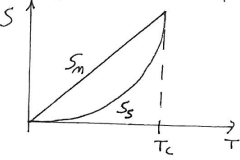
\includegraphics[width=0.4\linewidth]{Immagini - Capitolo 2/S(T).png}
    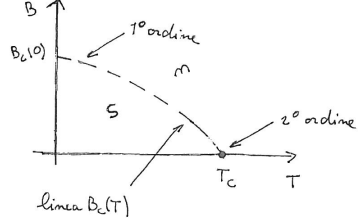
\includegraphics[width=0.4\linewidth]{Immagini - Capitolo 2/B(T).png}
    \caption{andamento in funzione della temperatura: (i) dell'entropia  per le fase normale e di superconduzione; (ii) del campo magnetico.}
    \label{fig: S(T) e B(T)}
\end{figure}

\subsection{Equazioni di London}
L'effetto Meissner-Ochsenfeld è il punto di partenza per la derivazione delle equazioni di London. Si considera un conduttore ideale, quindi, avendo resistenza nulla, le collisioni elettrone-elettrone ed elettrone-reticolo sono nulle. La seconda legge di Newton per il singolo elettrone di massa $m$ è semplicemente $m\va = -e\vE$. Definendo la densità di corrente $\vJ  = -ne\vv$, tale equazione si può riscrivere come
\begin{equation}
    \frac{\p\vJ}{\p t} = \frac{ne^2}{m}\vE.
\end{equation}
Supponendo che quest'ultima sia valida anche per i superconduttori, si trova la prima equazione di London
\begin{equation}
\label{eq: I equazione di London}
    \frac{\p\vJ}{\p t} = \frac{n_Se^2_S}{m_S}\vE,
\end{equation}
dove $n_S = n/2$, $e_S = 2e$ e $m_S = 2m$, dato che in questo regime i portatori di carica sono le coppie di Cooper, come descritto dalla teoria BCS. Diversamente da un conduttore normale, non è la corrente ad essere proporzionale al campo elettrico, ma lo è la sua derivata. Ad ogni modo, la prima equazione di London dà l'impressione che la corrente di un superconduttore possa crescere indefinitamente. In realtà, proprio perché la resistenza è nulla, anche il campo elettrico $\vE$ si annulla nello stato stazionario. Quindi, la variazione temporale di $\vJ$ si annulla, per cui la corrente rimane costante ed è esclusivamente determinata dalla sorgente. 

Si riparte adesso dalla terza equazione di Maxwell $\nabla \times \vE = -\p\vB/\p t$, dalla quale, moltiplicando per $n_Se^2_S/m_S$, si trova
\begin{equation}
    \frac{\p}{\p t}\bigg(\nabla \times \vJ_S + \frac{n_Se_S^2}{m_S}\vB\bigg) = 0.
\end{equation}
All'interno di un conduttore ideale, il flusso attraverso un circuito arbitrario non può variare nel tempo. Tuttavia, per un superconduttore, il campo magnetico all'interno non solo è costante, ma è proprio nullo. Da questo si trova la seconda equazione di London
\begin{equation}
\label{eq: II equazione di London}
    \nabla \times \vJ_S + \frac{n_Se_S^2}{m_S}\vB = 0.
\end{equation}
Dalla relazione $\vB = \nabla \times \vA$ si ha 
\begin{equation}
    \nabla \times \bigg(\vJ_S + \frac{n_Se_S^2}{m_S}\vA\bigg) = 0,
\end{equation}
da cui si trova immediatamente, imponendo il gauge di London $\nabla \cdot \vA = 0$, la forma della densità di corrente 
\begin{equation}
    \vJ_S = -\frac{n_Se_S^2}{m_S}\vA.
\end{equation}
Di conseguenza, dall'equazione di Maxwell per il potenziale vettore
\begin{equation}
    \square\vA = \nabla^2\vA - \cancelto{0}{\frac{1}{c^2}\frac{\p^2\vA}{\p t^2}} = -\mu_0\vJ_s = \frac{\mu_0n_Se_S^2}{m_S}\vA
\end{equation}
si trova l'equazione di Klein-Gordon per tale campo
\begin{equation}
    \bigg(\nabla^2 - \frac{c^2m_\gamma^2}{\hbar^2}\bigg)\vA = 0,\quad m_\gamma \equiv \sqrt{\frac{\mu_0n_Se_S^2}{m_S}}\frac{\hbar}{c}.
\end{equation}
Da questo risultato si conclude che in un superconduttore dove si verifica l'effetto di Meissner-Ochsenfeld corrisponde all'acquisizione da parte dei fotoni al suo interno di una massa pari a $m_\gamma$, in analogia con il meccanismo di Higgs-Anderson in Teoria dei campi. 

Una delle applicazioni più importanti della seconda equazione di London è la descrizione dello schermaggio nei superconduttori nello stato di Meissner. Fino ad ora si è sostenuto che il campo magnetico fosse completamente espulso in tale stato; tuttavia, se ciò fosse vero, una corrente di densità infinita dovrebbe circolare sulla superficie del superconduttore. Per discutere questo fenomeno, si assume che il superconduttore occupi lo spazio per $x > 0$ e che il campo magnetico sia $\vB = (0,0,B_{0z})$, come mostrato in figura \ref{fig: lunghezza di penetrazione}.
\begin{figure}[h]
    \centering
    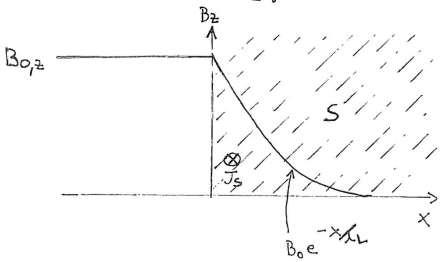
\includegraphics[width=0.5\linewidth]{Immagini - Capitolo 2/lunghezza di penetrazione.png}
    \caption{andamento del campo magnetico $\vB$ in un superconduttore.}
    \label{fig: lunghezza di penetrazione}
\end{figure}
Se si inserisce la seconda equazione di London nella quarta equazione di Maxwell $\nabla \times \vB = \mu_0\vJ_S$ si ha
\begin{equation}
    \nabla \times \nabla \times \vB + \frac{\mu_0n_Se_S^2}{m_S}\vB = 0,
\end{equation}
da cui, poiché $\nabla \times \nabla \times \vf = \nabla(\nabla \cdot \vf) - \nabla^2\vf$ e $\nabla \cdot \vB = 0$, si trova
\begin{equation}
    \begin{split}
        \nabla^2\vB - \frac{\mu_0n_Se_S^2}{m_S}\vB = \frac{d^2B_z(x)}{dx^2} - \frac{B_z(x)}{\Lambda_L^2} = 0,\quad \Lambda_L = \sqrt{\frac{m_s}{\mu_0n_Se_S^2}},
    \end{split}
\end{equation}
dove $\Lambda_L$ è la lunghezza di penetrazione di London, la quale è legata alla massa acquisita dal fotone da $\Lambda_L = \hbar/cm_\gamma$. La soluzione dell'equazione in $B_z(x)$ è
\begin{equation}
    B_z(x) = B_{0z}e^{-x/\Lambda_L},
\end{equation}
che inserita nella quarta equazione di Maxwell restituisce la variazione spaziale della corrente di screening
\begin{equation}
    J_{S,y}(x) = J_{0y}e^{-x/\Lambda_L} = \frac{B_{0z}}{\mu_0\Lambda_L}e^{-x/\Lambda_L}.
\end{equation}
Quindi, sia il campo magnetico che la densità di corrente decrescono esponenzialmente all'interno di un superconduttore con una lunghezza di penetrazione $\Lambda_L$ data dall'inverso della massa acquisita dal fotone in tale mezzo. Inoltre, il campo magnetico applicato e la corrente sono proporzionali, $B_{0z} = \mu_0\Lambda_LJ_{0y}$.

\section{Modello di Landau-Ginzburg}
La teoria di Landau-Ginzburg per la superconduttività è stata formulata utilizzando un approccio generale alle transizioni di fase del secondo ordine. Tale teoria è caratterizzata da un parametro d'ordine il cui valore all'equilibrio è nullo nella fase disordinata a $T \ge T_c$ ma diventa diverso da zero per $T < T_c$. In particolare, per la superconduttività, la teoria di Landau-Ginzburg postula l'esistenza di un parametro d'ordine $\psi$, il quale caratterizza lo stato superconduttore nello stesso modo in cui la magnetizzazione caratterizza lo stato di un ferromagnete. Si assume quindi che all'equilibrio
\begin{equation} 
    \begin{cases}
        \psi = 0, \quad T \ge T_c \\
        \psi \neq 0, \quad T \le T_c
    \end{cases},\quad \psi \equiv \psi_0(T).
\end{equation}
Il parametro d'ordine è postulato essere complesso, facendo riferimento ad una funzione d'onda macroscopica per il superconduttore analoga a quella dell'elio-II. Inizialmente, il significato di $\psi$ non era chiaro, ma con lo sviluppo della teoria BCS si intuì fosse legato alla densità di coppie di Cooper. Si assume che l'energia libera del superconduttore dipenda in modo ``smooth'' dal parametro d'ordine. Inoltre, poiché $\psi$ è complesso, l'energia libera deve dipendere solo da $\psi^*\psi = |\psi|^2$, per cui
\begin{equation}
   \Delta f \equiv f_S(T) - f_N(T) = a(T)|\psi|^2 + \frac{b(T)}{2}|\psi|^4 + o(|\psi|^6),
\end{equation}
dove $f = F/V$ è l'energia libera di Helmoltz e $f_S$ ed $f_n$ sono quelle relative allo stato superconduttivo e normale, rispettivamente, mentre i parametri $a(T)$ e $b(T)$ sono parametri fenomenologici che dipendono in modo ``smooth'' dalla temperatura $T$. Se si grafica l'andamento di $\Delta f$ in funzione di $|\psi|$, mostrato in figura \ref{fig: energia di Helmoltz (teoria L-G)}, si presentano due casi:
\begin{enumerate}
    \item se $a(T) > 0$, la curva ha un minimo in $|\psi|^2 = |\psi_0|^2 = 0$ e $f_S > f_N$;
    \item se $a(T) < 0$, la curva ha un minimo in $|\psi|^2 = |\psi_0|^2 = -a(T)/b(T)$.
\end{enumerate}
Nel modello di Landau-Ginzburg si assume che 
\begin{equation}
    \begin{cases}
        a(T) > 0,\quad T > T_c \\
        a(T) = 0,\quad T = T_c \\
        a(T) < 0,\quad T < T_c
    \end{cases}
\end{equation}
e che $b(T)$ vari lentamente attorno a $T = T_c$, per cui 
\begin{equation}
    \begin{cases}
        a(T) \simeq \tilde{a}(T - T_c) \\
        b(T) \simeq b
    \end{cases},
\end{equation}
mentre
\begin{equation}
    |\psi_0| = \begin{cases}
        0,\quad T \ge T_c \\
        \bigg(\dfrac{\tilde{a}}{b}\bigg)^{1/2}(T - T_c)^{1/2},\quad T < T_c
    \end{cases},
\end{equation}
dove $|\psi_0|$ minimizza $\Delta f \equiv f_S - f_N$.
\begin{figure}[h]
    \centering
    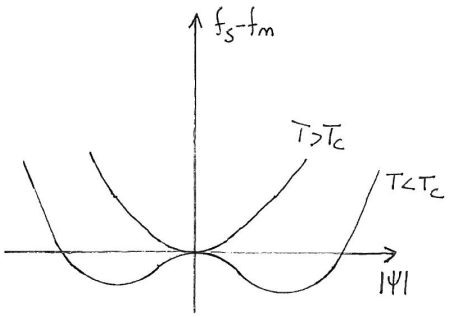
\includegraphics[width=0.4\linewidth]{Immagini - Capitolo 2/energia di Helmoltz (teoria L-G).png}
    \caption{andamento di $\Delta f \equiv f_S - f_N$ in funzione di $|\psi|$.}
    \label{fig: energia di Helmoltz (teoria L-G)}
\end{figure}
Sostituendo $|\psi|^2 = |\psi_0|^2 = \tilde{a}(T_c - T)/b$, si ha
\begin{equation}
    \begin{split}
        f_S(T) - f_N(T) &= \tilde{a}(T - T_c)\bigg(\frac{\tilde{a}}{b}\bigg)(T_c - T) + \frac{b}{2}\bigg(\frac{\tilde{a}}{b}\bigg)^2(T_c - T)^2 \\
        &= -\frac{\tilde{a}^2}{2b}(T - T_c)^2.
    \end{split}
\end{equation}
Poiché, la differenza di energia libera di Gibbs è
\begin{equation}
    G_N(0,T) - G_S(0,T) = \frac{\mu_0H_c^2V}{2} = F_N(0,T) - F_S(0,T) + \mu_0 \cancelto{0}{(\vH \cdot \vM)},
\end{equation}
si ha
\begin{equation}
    F_S(0,T) - F_N(0,T) = -\frac{\mu_0VH_c^2}{2},
\end{equation}
che confrontata con $\Delta f(0,T) = -\tilde{a}^2(T - T_c)^2/2b$, restituisce
\begin{equation}
    H_c = \frac{\tilde{a}(T_c - T)}{\sqrt{\mu_0 b}},
\end{equation}
che coincide con l'approssimazione lineare a $T \simeq T_c$ di 
\begin{equation}
    H_c(T) = H_c(0)\bigg(1 - \frac{T^2}{T_c^2}\bigg) = \frac{H_c(0)}{T_c^2}(T_c - T)(T_c + T) \simeq \frac{2H_c(0)}{T_c}(T_c - T).
\end{equation}

\subsection{Sistemi non omogenei}
Per completare la teoria di Landau-Ginzburg per la superconduttività, si permette al parametro d'ordine $\psi$ di dipendere anche dalle coordinate spaziali $\vr$. La teoria in questo modo comincia ad assomigliare alla teoria dei superfluidi 
\begin{equation}
    f_S(T,\vr) - f_N(T,\vr) = \frac{\hbar^2}{2m^*}|\nabla\psi(\vr)|^2 + a(T)|\psi(\vr)|^2 + \frac{b(T)}{2}|\psi(\vr)|^4,
\end{equation}
dove si nota come ponendo $\psi(\vr) = \psi$ si ritorni al caso precedente. Inoltre, il parametro $m^*$, avente le dimensioni di una massa, determina il costo di energia associato a gradienti non nulli di $\psi(\vr)$. Quindi, $m^*$ gioca il ruolo di massa efficace nel sistema quantistico con funzione d'onda macroscopica $\psi(\vr)$. L'energia totale del sistema è
\begin{equation}
    F_S(T) = F_N(T) + \int_Vd^3r\,\bigg[-\frac{\hbar^2}{2m^*}\psi^*\nabla^2\psi + a(T)\psi^*\psi + \frac{b}{2}(\psi^*\psi)^2\bigg]
\end{equation}
La configurazione di equilibrio termodinamico si ha imponendo
\begin{equation}
    \frac{\delta F_S}{\delta \psi^*} = 0,
\end{equation}
ossia richiedendo che la funzione integranda sia minima; da qui si ottiene
\begin{equation}
    \bigg[-\frac{\hbar^2}{2m^*}\nabla^2 + a + b|\psi(\vr)|^2\bigg]\psi(\vr) = 0,
\end{equation}
che coincide all'equazione stazionaria di Gross-Pitaevskii per i gasi diluiti a bassa temperatura.

\subsection{Interfaccia nei superconduttori}
L'equazione non lineare di Schr\"odinger ha svariate applicazioni, ad esempio può essere usata per studiare la risposta del parametro d'ordine ad una perturbazione esterna. Si consideri un modello semplice di interfaccia tra un superconduttore ed un conduttore normale, come mostrato in figura \ref{fig: interfaccia SC I}; l'equazione da risolvere è
\begin{equation}
    -\frac{\hbar^2}{2m^*}\frac{d^2\psi(x)}{dx^2} + a(T)\psi(x) + b\psi(x)^3 = 0,
\end{equation}
con le condizioni al contorno
\begin{equation}
    \begin{cases}
        \psi(x) \neq 0,\quad x > 0 \\
        \psi(x) = 0,\quad x < 0
    \end{cases}.
\end{equation}
\begin{figure}[h]
    \centering
    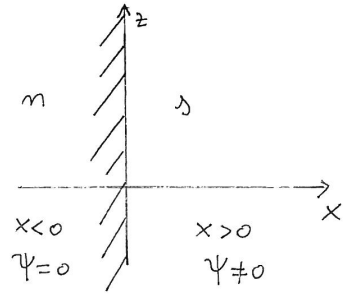
\includegraphics[width=0.35\linewidth]{Immagini - Capitolo 2/interfaccia SC I.png}
    \caption{interfaccia tra un superconduttore ed un conduttore normale.}
    \label{fig: interfaccia SC I}
\end{figure}

Ricordando l'equazione soddisfatta da $f(z) = \tanh{z}$,
\begin{equation}
    \frac{df(z)}{dz} = 1 - f(z)^2,
\end{equation}
da cui si può calcolare
\begin{equation}
    \begin{split}
        \frac{d^2f(z)}{dz^2} = -2f(z)[1 - f(z)^2] = -2f(x) + 2f(z)^3,
    \end{split}
\end{equation}
si trova un'equazione con la medesima forma di quella che si intende risolvere
\begin{equation}
    -\frac{d^2f(z)}{dz^2} - 2f(x) + 2f(z)^3 = 0.
\end{equation}
Usando infatti l'ansatz $\psi(x) = \alpha\phi(x\beta)$, e usando il fatto che $a(T) = -|a(T)|$, si ha
\begin{equation}
    \begin{split}
        -\frac{\hbar^2\beta^2\alpha}{2m^*}\frac{d^2\phi(x\beta)}{d(x\beta)^2} - |a(T)|\alpha\phi(x\beta) + \alpha^3b\phi(x\beta)^3 &= 0 \\
        -\frac{d^2\phi(x\beta)}{d(x\beta)^2} - \frac{|a(T)|}{\bigg(\dfrac{\hbar^2\beta^2}{2m^*}\bigg)}\phi(x\beta) + \frac{\alpha^2b}{\bigg(\dfrac{\hbar^2\beta^2}{2m^*}\bigg)}\phi(x\beta)^3 &= 0,
    \end{split}
\end{equation}
Quindi, definendo i parametri $\alpha$ e $\beta$ in modo opportuno imponendo
\begin{equation}
    \begin{cases}
        \dfrac{|a(T)|}{\bigg(\dfrac{\hbar^2\beta^2}{2m^*}\bigg)} = 2 \\[5ex]
        \dfrac{\alpha^2b}{\bigg(\dfrac{\hbar^2\beta^2}{2m^*}\bigg)} = 2
    \end{cases}\quad\Longrightarrow\quad
    \begin{cases}
        \alpha = \sqrt{\dfrac{|a(T)|}{b}} \\[2ex]
        \beta = \sqrt{\dfrac{|a(T)|m^*}{\hbar^2}}
    \end{cases},
\end{equation}
si trova la soluzione 
\begin{equation}
    \psi(x) = \sqrt{\frac{|a(T)|}{b}}\phi\bigg(x\sqrt{\frac{|a(T)|m^*}{\hbar^2}}\bigg) \equiv \psi_0\tanh{\bigg[\frac{x}{\sqrt{2}\xi(T)}\bigg]},
\end{equation}
dove si è definita la lunghezza di healing, o di coerenza, come 
\begin{equation}
    \xi(T) \equiv \frac{\hbar}{\sqrt{2m^*|a(T)|}} = \frac{\hbar}{\sqrt{2m^*\tilde{a}(T - T_c)}},
\end{equation}
che racchiude l'informazione di quanto la funzione d'onda cambi all'interfaccia rispetto allo stato lontano da essa, che tende a $\psi_0$, come mostrato in figura \ref{fig: parametro d'ordine SC in x}. Il fatto che $\xi(T) \propto |T - T_c|^{-1/2}$ implica che la lunghezza di healing diverge alla temperatura critica con un esponente critico pari a $-1/2$. Da questo risultato è possibile ottenere l'energia associata alla penetrazione dell'interfaccia all'interno del superconduttore in $x > 0$; in altre parole, si vuole determinare la differenza in energia tra le due configurazioni mostrate in figura \ref{fig: interfaccia SC II}. L'energia libera di bulk nel volume $V = \Sigma x_0$ è 
\begin{equation}
    F_S(0,T) - F_N(0,T) = -\mu_0\frac{VH_c^2}{2} = -\frac{a^2}{2b}\Sigma x_0,
\end{equation}
a cui corrisponde un'energia per unità di superficie 
\begin{equation}
    \sigma_{bulk} = \frac{F_S(0,T) - F_N(0,T)}{S} = -\int_0^{x_0}dx\,\frac{\mu_0H_c^2}{2}
\end{equation}
e una differenza di energia pari a 
\begin{equation}
    \begin{split}
        \sigma &= \sigma_\psi - \sigma_{bulk} \\
        &= \int_0^\infty dx\,\bigg[\frac{\hbar^2}{2m^*}\bigg(\frac{d\psi(x)}{dx}\bigg)^2 + a(T)\psi(x)^2 + \frac{b}{2}\psi(x)^4 + \frac{\mu_0H_c^2}{2}\bigg].
    \end{split}
\end{equation}
Quest'ultima, dal calcolo dovuto a de Gennes, risulta essere pari a
\begin{equation}
    \sigma \simeq (1.89)\times\frac{1}{2}\mu_0H_c^2\xi(T).
\end{equation}
\begin{figure}[h]
    \centering
    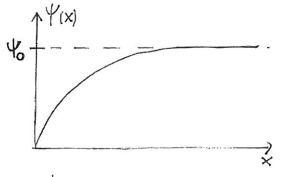
\includegraphics[width=0.4\linewidth]{Immagini - Capitolo 2/parametro d'ordine SC in x.png}
    \caption{andamento del parametro d'ordine $\psi$ in funzione di $x$.}
    \label{fig: parametro d'ordine SC in x}
\end{figure}
\begin{figure}[h]
    \centering
    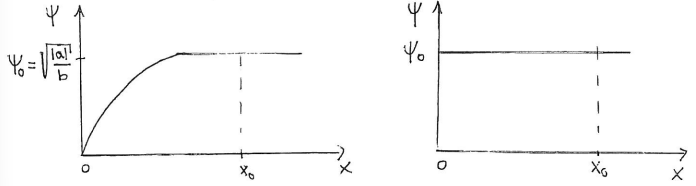
\includegraphics[width=0.9\linewidth]{Immagini - Capitolo 2/interfaccia SC II.png}
    \caption{configurazioni dove $\psi(x)$ è: (i) pari a $\sqrt{|a(T)|/b}$; (ii) costante.}
    \label{fig: interfaccia SC II}
\end{figure}

\subsection{Teoria di Landau-Ginzburg in campo magnetico}
La vera potenzialità dell'approccio di Landau e Ginzburg applicato ai superconduttori diventa evidente solo quando si inserisce il contributo del campo magnetico. Infatti, fino ad ora quanto discusso non include gli effetti legati alla caratteristica del superfluido di non essere neutro, ma carico, essendo appunto una supercorrente. L'introduzione del contributo di campo magnetico viene postulato da Landau e Ginzburg assumendo un accoppiamento minimo tra il parametro d'ordine $\psi(\vr)$ e $\vB$, ottenuto dalla sostituzione
\begin{equation}
    -i\hbar\nabla \to -i\hbar\nabla - q\vA,
\end{equation}
equivalente a considerare $\psi(\vr)$ come una funzione d'onda di particelle cariche con carica $q$. In particolare, risultava che per i tutti i superconduttori la carica era $q = 2e \equiv e_S$, per cui
\begin{equation}
    -i\hbar\nabla \to -i\hbar\nabla - 2e\vA.
\end{equation}
Di nuovo, la spiegazione di questo avvenne con lo sviluppo della teoria BCS e con la comprensione del legame tra tale teoria e quella di Landau-Ginzburg. Ad ogni modo, ora l'energia libera nella teoria di Landau-Ginzburg è
\begin{equation}
    f_S(T) - f_N(T) = \frac{1}{2m^*}|(-i\hbar\nabla - 2e\vA)\psi(\vr)|^2 + a(T)|\psi(\vr)|^2 + \frac{b}{2}|\psi(\vr)|^4.
\end{equation}
Quest'ultima espressione contiene l'accoppiamento tra la funzione d'onda del condensato e il campo magnetico attraverso il potenziale vettore $\vA$, con $\vB = \nabla \times \vA$. Tuttavia, a questo punto non è possibile separare completamente il condensato dal campo magnetico e nel calcolo dell'energia libera bisogna pertanto includere anche il termine 
\begin{equation}
    \Delta F_{\vB} = \frac{1}{2\mu_0}\int_{\R^3} d^3r\,\vB(\vr)^2,
\end{equation}
dove l'integrale in $\R^3$ è inteso su tutto lo spazio. Quindi, così facendo si ottiene che $\Delta F \equiv F_S(T) - F_N(T)$ è data da
\begin{equation}
    \begin{split}
        \Delta F &= \int_V d^3r\,\bigg[\frac{1}{2m^*}|(-i\hbar\nabla - 2e\vA)\psi(\vr)|^2 + a(T)|\psi(\vr)|^2 + \frac{b}{2}|\psi(\vr)|^4\bigg] \\
        &+ \frac{1}{2\mu_0}\int_{\R^3} d^3r\,\vB(\vr)^2.
    \end{split}
\end{equation}
Quindi, $\Delta F$ è costituita da tre contributi $\Delta F = \Delta F_\psi + \Delta F_{\vB} + \Delta F_{int}$, dove 
\begin{align}
    \Delta F_\psi &= \int_V d^3r\,\bigg[\frac{\hbar^2}{2m}|\nabla^2\psi| + a(T)|\psi(\vr)|^2 + \frac{b}{2}|\psi(\vr)|^4\bigg], \\
    \Delta F_{\vB} &= \frac{1}{2\mu_0}\int_{\R^3} d^3r\,\vB(\vr)^2, \\
    \begin{split}
        \Delta F_{int} &= \int_V\frac{d^3r}{2m^*}[-2ei\hbar\nabla\psi^*(\vr)\vA\psi(\vr) + 2ei\hbar\nabla\psi(\vr)(\vA\psi(\vr))^* \\
        &+ (2e)^2|\psi(\vr)|^2(\vA \cdot \vA)] \\
        &= \int_V d^3r\,\bigg[\frac{2ei\hbar}{2m^*}(\psi^*\nabla\psi - \psi\nabla\psi^*)\cdot\vA + \frac{(2e)^2}{2m^*}|\psi|^2(\vA\cdot\vA)\bigg].
    \end{split}
\end{align}
In particolare, l'energia di interazione può essere sempre scritta come
\begin{equation}
    F_{int} = -\int_Vd^3r\,\vJ_S\cdot\vA,
\end{equation}
ovvero
\begin{equation}
    \frac{\delta F_{int}}{\delta \vA} = -\vJ_S,
\end{equation}
per cui la densità di supercorrente è
\begin{equation}
    \vJ_S = -\frac{2ei\hbar}{2m^*}(\psi^*\nabla\psi - \psi\nabla\psi^*) - \frac{(2e)^2}{m^*}|\psi|^2\vA.
\end{equation}
Inoltre, ponendo $\psi(\vr) = |\psi(\vr)|e^{i\theta}$, il termine $\psi^*\nabla\psi - \psi\nabla\psi^* = 2i|\psi(\vr)|\nabla\theta$, quindi si può scrivere $\vJ_S$ come
\begin{equation}
    \begin{split}
        \vJ_S &= \frac{2e\hbar}{m^*}|\psi(\vr)|^2\nabla\theta - \frac{(2e)^2}{m^*}|\psi(\vr)|^2\vA \\
        &= \frac{(2e)^2}{m^*}|\psi(\vr)|^2\bigg(\frac{\hbar}{2e}\nabla\theta - \vA\bigg).
    \end{split}
\end{equation}
Il parametro d'ordine $\psi(\vr)$ è soluzione dell'equazione di Gross-Pitaesvkii con accoppiamento minimale
\begin{equation}
    -\frac{\hbar^2}{2m^*}\bigg(\nabla - \frac{2ei}{\hbar}\vA\bigg)^2 + [a(T) + b|\psi(\vr)|^2]\psi(\vr) = 0.
\end{equation}

\subsection{Simmetria di gauge}
Il parametro d'ordine dei superconduttori $\psi(\vr) = |\psi(\vr)|e^{i\theta(\vr)}$ ha un'ampiezza ed una fase. Da questo punto di vista la situazione è molto simile a quella dei superfluidi, ma con una differenza sostanziale. Per capire di cosa si tratta si consideri l'operatore momento 
\begin{equation}
    \hatp = -i\hbar\nabla - 2e\vA,
\end{equation}
se si trasforma $\psi(\vr)$ con un fattore di fase moltiplicativo $\psi(\vr) \to \psi(\vr)e^{i\chi(\vr)}$ si ha 
\begin{equation}
    \begin{split}
        \hatp\psi(\vr)e^{i\chi(\vr)} &= e^{i\chi(\vr)}(-i\hbar\nabla - 2e\vA)\psi(\vr) + \hbar\psi(\vr)e^{i\chi(\vr)}\nabla\chi(\vr) \\
        &= e^{i\chi(\vr)}\bigg[-i\hbar\nabla - 2e\bigg(\vA - \frac{\hbar}{2e}\nabla\chi(\vr)\bigg)\bigg]\psi(\vr),
    \end{split}
\end{equation}
da cui si può dedurre che, se si operano simultaneamente le trasformazioni di gauge
\begin{equation}
\label{eq: trasformazione di gauge locale superconduttori}
    \begin{cases}
        \psi(\vr) \to \psi(\vr)e^{i\chi(\vr)} \\[2ex]
        \vA(\vr) \to \vA(\vr) + \dfrac{\hbar}{2e}\nabla\chi(\vr)
    \end{cases},
\end{equation}
la teoria presenta un'invarianza di gauge locale; infatti, sia la fase della funzione d'onda $e^{i\chi(\vr)}$ che il potenziale vettore $\vA$ dipendono dalla scelta del gauge, ma tutte le osservabili sono invarianti. Ora si consideri la corrente
\begin{equation}
    \vJ_S = \frac{(2e)^2}{m^*}|\psi(\vr)|^2\bigg(\frac{\hbar}{2e}\nabla\theta - \vA\bigg),
\end{equation}
che è come ci si aspetta invariante per la trasformazione di gauge locale \eqref{eq: trasformazione di gauge locale superconduttori}, e se ne calcoli il rotore
\begin{equation}
    \nabla \times \vJ_S = 0 - \frac{(2e)^2}{m^*}|\psi_0|^2(\nabla \times \vA) = -\frac{(2e)^2}{m^*}|\psi_0|^2\vB,
\end{equation}
dove si è assunto che $|\psi|^2 = |\psi_0|^2 = costante$ e si è usata la proprietà $\nabla \times (\nabla\vf) = 0$ per ogni $\vf$. Si nota che tale rotore coincide con la seconda equazione di London \eqref{eq: II equazione di London}, a patto di identificare
\begin{equation}
    m_S = m^* = 2m_e,\quad e_S = 2e,\quad n_S = |\psi_0|^2.
\end{equation}
Quindi, poiché la seconda equazione di London è equivalente all'effetto di Meissner-Ochesenfeld, si è così verificato che il modello di Landau e Ginzburg descrive la fisica dei superconduttori. Inoltre, considerando il regime stazionario dove si ha $\p_t\vE = 0$ e assumendo l'assenza di correnti esterne, si ha che
\begin{equation}
    \nabla \times \vB = \mu_0\vJ_s\quad \Longrightarrow\quad \nabla \times \nabla \times \vB = \mu_0(\nabla \times \vJ_s),
\end{equation}
per cui 
\begin{equation}
    \nabla^2\vB = -\frac{(2e)^2\mu_0}{m^*}|\psi_0|^2\vB = -\frac{c^2m_\gamma^2}{\hbar^2}\vB,
\end{equation}
che riarrangiata corrisponde all'equazione
\begin{equation}
    \nabla^2\vB + \frac{c^2m_\gamma^2}{\hbar^2}\vB = 0,\quad m_\gamma = \frac{\hbar}{c}\sqrt{\frac{\mu_0(2e)^2|\psi_0|^2}{m}}.
\end{equation}
Dunque, la massa acquisita dal fotone tramite il meccanismo di Anderson-Higgs è proporzionale al modulo del parametro d'ordine all'equilibrio. L'acquisizione di massa da parte del fotone in particolare deriva dalla variazione di fase della funzione d'onda, questo cambiamento longitudinale può essere assorbito da $\vA$: nel vuoto il campo è ortogonale alla direzione di propagazione, ma adesso il campo acquisisce un grado di libertà longitudinale, passando da due a tre gradi di libertà, permettendogli appunto di acquisire massa.
\begin{obs}
    Si può seguire un procedimento analogo per il potenziale vettore $\vA$ nel caso omogeneo con $\theta = costante$ ponendosi nel gauge di London con $\nabla \cdot \vA = 0$.
\end{obs}

\section{Quantizzazione del flusso magnetico}
In generale, la fase $\theta(\vr)$ della funzione d'onda macroscopica nei superconduttori è ben definita a meno di multipli di $2\pi$. La differenza $\Delta\theta$ tra due punti del superconduttore si ottiene calcolando l'integrale di linea sulla curva $L$ che unisce i due punti 
\begin{equation}
    \Delta\theta = \oint_L\nabla\theta \cdot d\vl = 2\pi n,\quad n \in \Z.
\end{equation}
Per dimostrare la quantizzazione del flusso di campo magnetico, si consideri un superconduttore a forma toroidale, quindi un dominio connesso, ma non semplicemente. Immergendo il toroide in un campo magnetico esterno, che passa attraverso il foro, mentre all'esterno viene deviato. L'esistenza di una funzione d'onda macroscopica ha una conseguenza importante per il flusso del flusso di campo magnetico all'interno del foro. Si consideri ora di nuovo l'espressione della corrente
\begin{equation}
    \vJ_S = \frac{(2e)^2}{m^*}|\psi|^2\bigg(\frac{\hbar}{2e}\nabla\theta - \vA\bigg),
\end{equation}
integrandola su un cammino chiuso all'interno del superconduttore dove $\vJ_S = \vo$, assumendo $|\psi|^2 = |\psi_0|^2 = costante$, si ha
\begin{equation}
    \oint_L\bigg(\vA - \frac{h}{2e}\nabla\theta\bigg)\cdot d\vl = 0,
\end{equation}
da cui, calcolando gli integrali dei due termini separatamente, si hanno
\begin{equation}
    \frac{\hbar}{2e}\oint_L\nabla\theta\cdot d\vl = \dfrac{nh}{2e},\quad n \in \Z
\end{equation}
e
\begin{equation}
    \oint_L \vA \cdot d\vl = \int_\Sigma(\nabla \times \vA)\cdot d\bm{\Sigma} = \int_\Sigma\vB \cdot \bm{\Sigma} = \Phi.
\end{equation}
Dunque, il flusso di campo magnetico all'interno del foro è un multiplo intero di un quanto di flusso $\Phi_0$, chiamato spesso ``flussone'', dato da
\begin{equation}
    \Phi_0 = \frac{h}{2e} \simeq \SI{2.05e-15}{\tesla\meter\squared},
\end{equation}

\subsection{Effetto Josephson}
La previsione teorica di Josephson consisteva tra due materiali superconduttori separati da una piccola barriera di isolante si instaura una corrente spontanea $I_S = I_C\sin{(\Delta\theta_0)}$, dove $\Delta\theta_0$ è la differenza di fase tra le due funzioni d'onda.

Inizialmente, quello che si cerca di capire una volta ipotizzato che ai superconduttori può essere associata una funzione d'onda macroscopica e complessa, è cercare la prova dell'esistenza o meno di una fase. L'effetto Josephson può essere indotto riducendo lo spessore dello strato isolante tra due superconduttori a circa $\SI{10}{\angstrom}$, si ottiene una sovrapposizione non nulla delle funzioni d'onda macroscopiche e si instaura la corrente di superconduzione, oppure al contrario instaurando una differenza di potenziale tra i due materiali, che a sua volta genera una supercorrente alternata con frequenza $\omega = 2e\Delta V/\hbar$. L'apparato sperimentale consiste nel porre a contatto due cavi superconduttori, tra i quali si deposita uno strato di ossido molto sottile, così che le funzioni d'onda si sovrappongano nelle vicinanze di questa giunzione isolante, chiamata giunzione di Josephson. Si preparano quindi due superconduttori inizialmente separati e si abbassa la temperatura sotto la soglia critica, cosicché la funzione d'onda acquisisca un valore di aspettazione non nullo nello stato fondamentale. 

Si considera ora l'equazione di Schr\"odinger per due superconduttori accoppiati da un termine di interazione 
\begin{equation}
\label{eq: equazioni superconduttori giunzione di Josephson}
    \begin{cases}
        i\hbar\dfrac{\p \psi_1}{\p t} = \mu_1\psi_1 + k\psi_2 \\[2ex]
        i\hbar\dfrac{\p \psi_2}{\p t} = \mu_2\psi_2 + k\psi_1
    \end{cases},
\end{equation}
dove $\mu_1$ e $\mu_2$ rappresentano i potenziali chimici dei due superconduttori, mentre la costante $k$ riflette l'intensità dell'accoppiamento. In assenza della giunzione, le due funzioni d'onda sono descritte dalle leggi 
\begin{equation}
    \psi_i(t) = \psi_{0,i}e^{-i\mu_it/\hbar},\quad i = \{1,2\}.
\end{equation}
Nel caso di una differenza di potenziale alla giunzione nulla, i potenziali chimici sono identici $\mu_1 = \mu_2 \equiv \mu$, invece una differenza di potenziale $\Delta V \neq 0$ sposta i livelli di Fermi dei due superconduttori in modo che $\mu_2 - \mu_1 = -2e\Delta V$. Inoltre, per semplificare la trattazione, si assume che i due superconduttori siano dello stesso materiale e abbiano la medesima densità di portatori di supercorrente, $n_{S_1} = n_{S_2} \equiv n_S$. Quindi, se si inserisce $\psi_i(t) = \sqrt{n_{S_i}(t)}\exp{[i\theta_i(t)]}$, nelle equazioni accoppiate \eqref{eq: equazioni superconduttori giunzione di Josephson} si hanno
\begin{equation}
    \begin{cases}
        i\hbar\dfrac{\p}{\p t}[\sqrt{n_{S_1}}(t)]e^{i\theta_1(t)} - \hbar\dot{\theta}_1\sqrt{n_S}e^{i\theta_1} = \mu_1\sqrt{n_S}e^{i\theta_1} + k\sqrt{n_S}e^{i\theta_2} \\[2ex]
        i\hbar\dfrac{\p}{\p t}[\sqrt{n_{S_2}}(t)]e^{i\theta_2(t)} - \hbar\dot{\theta}_2\sqrt{n_S}e^{i\theta_2} = \mu_2\sqrt{n_S}e^{i\theta_2} + k\sqrt{n_S}e^{i\theta_1}
    \end{cases}
\end{equation}
che si possono riscrivere come
\begin{equation}
    \begin{cases}
        \dfrac{i\hbar}{2}\dot{n}_{S_1} - \hbar\dot{\theta}_1n_S = \mu_1 n_S + kn_Se^{i(\theta_2 - \theta_1)} \\[2ex]
        \dfrac{i\hbar}{2}\dot{n}_{S_2} - \hbar\dot{\theta}_2n_S = \mu_2 n_S + kn_Se^{i(\theta_1 - \theta_2)}
    \end{cases},
\end{equation}
separando poi la parte reale da quella immaginaria rispettivamente 
\begin{equation}
    \Re :
    \begin{cases}
        \dot{\theta}_1 = -\dfrac{\mu_1}{\hbar} - \dfrac{k}{\hbar}\cos{(\theta_2 - \theta_1)} \\[2ex]
        \dot{\theta}_2 = -\dfrac{\mu_2}{\hbar} - \dfrac{k}{\hbar}\cos{(\theta_2 - \theta_1)}
    \end{cases},\quad \Im :
    \begin{cases}
        \dot{n}_{S_1} = \dfrac{2k}{\hbar}n_S\sin{(\theta_2 - \theta_1)} \\[2ex]
        \dot{n}_{S_2} = -\dot{n}_{S_1}
    \end{cases}
\end{equation}
e combinandole, si ottengono le equazioni
\begin{equation}
\label{eq: equazioni effetto Josephson}
    \begin{cases}
        \dot{n}_{S_1} = \dfrac{2k}{\hbar}\sin{(\theta_2 - \theta_1)} = -\dot{n}_{S_2} \\[2ex]
        \hbar(\dot{\theta}_2 - \dot{\theta}_1) = -(\mu_2 - \mu_1) = 2e\Delta V
    \end{cases}.
\end{equation}
Si considera come primo caso quello in cui la differenza di potenziale alla giunzione è nulla. Se $\Delta V = 0$, allora la differenza di fase è indipendente dal tempo, per cui anche $\dot{n}_S$ è costante e nella giunzione si instaura una supercorrente continua. Essendo tale corrente proporzionale a sua volta a $\dot{n}_{S_1}$ si può scrivere
    \begin{equation}
        I_S = I_C\sin{(\theta_2 - \theta_1)}.
    \end{equation}
Questo fenomeno, ossia lo scorrere di una corrente attraverso un contatto isolante senza generare una differenza di potenziale prende il nome di ``effetto Josephson in DC''. Negli esperimenti si opera tipicamente al contrario imponendo una corrente $I_S$ attraverso la giunzione e poi misurando $\Delta V$, dove $\Delta V = 0$ per $I_S < I_C$, mentre $\Delta V \neq 0$ per $I_S > I_C$. In particolare, la corrente critica $I_C$ dipende dalla densità $n_S$, dall'area di contatto $A$ e dalla costante di accoppiamento $k$. Il motivo per cui $I_C$ è chiamata corrente critica è chiarito in figura \ref{fig: effetto Josephson DC} che rappresenta una giunzione di Josephson formata da due cavi di superconduttore separati da un sottile strato isolante.
\begin{figure}[h]
    \centering
    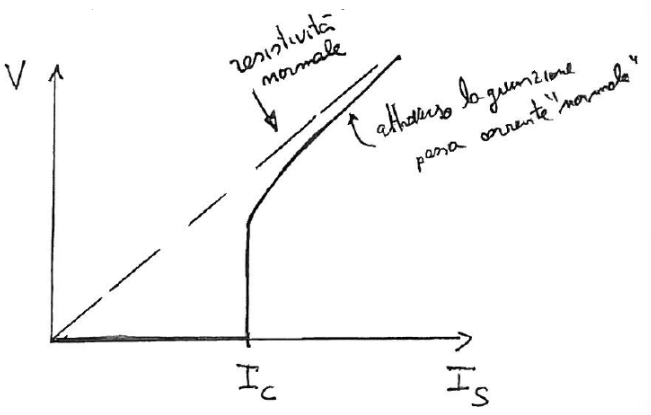
\includegraphics[width=0.35\linewidth]{Immagini - Capitolo 2/effetto Josephson DC.png}
    \caption{andamento di $\Delta V$ alla giunzione in funzione di $I_S$.}
    \label{fig: effetto Josephson DC}
\end{figure}
Fintanto che la corrente è minore del valore critico $I_C$ non si osserva sperimentalmente alcuna differenza di potenziale alla giunzione, tuttavia incrementando l'intensità della corrente oltre $I_C$ la differenza di potenziale balza ad un valore finito, dipendente dalle caratteristiche della giunzione stessa, conseguente in un passaggio di corrente normale. Nel caso in cui $I_S > I_C$ però Josephson scoprì anche una seconda conseguenza dell'effetto tunnel della giunzione: una differenza di potenziale tra i due superconduttori implica che le funzioni d'onda diventano dipendenti dal tempo. Integrando quindi la seconda equazione del sistema \eqref{eq: equazioni effetto Josephson} si ha 
\begin{equation}
    \theta_2 - \theta_1 = \frac{2e\Delta V}{\hbar}t + \theta_0 = \omega_jt + \theta_0.
\end{equation}
Quindi, la differenza di fase cresce linearmente nel tempo e si ha che la corrente è
\begin{equation}
    I_N = I_C\sin{(\omega_jt + \theta_0)}.
\end{equation}
Questo fenomeno invece prende il nome di ``effetto Josephson in AC''. La frequenza $\nu_j \equiv \omega_j/2\pi$ è molto elevata $\nu_j \simeq \SI{48}{\giga\hertz}$ per $\Delta V = \SI{100}{\micro\volt}$. 
\begin{figure}[h]
    \centering
    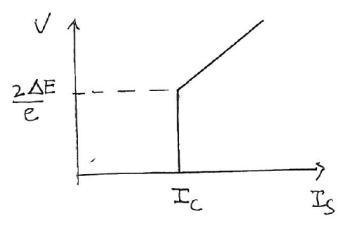
\includegraphics[width=0.35\linewidth]{Immagini - Capitolo 2/effetto Josephson giunzione ideale.png}
    \caption{andamento di $\Delta V$ in funzione di $I_S$ per una giunzione ideale.}
    \label{fig: effetto Josephson giunzione ideale}
\end{figure}

A temperatura $T = \SI{0}{\kelvin}$, in una giunzione ideale, ci si aspetta un comportamento del tipo mostrato in figura \ref{fig: effetto Josephson giunzione ideale}, dove $\Delta E$ è l'energia necessaria per rompere una coppia di Cooper e dove:
\begin{enumerate}
    \item per $I_S < I_C$ la corrente attraverso la giunzione è una supercorrente che non genera una differenza di potenziale;
    \item per $I_S > I_C$ la corrente attraverso la giunzione è una corrente normale, per cui le coppie di Cooper si spezzano.
\end{enumerate}

\subsection{Interferenza quantistica}
L'effetto Josephson è un elemento chiave in molte applicazioni riguardanti l'informatica quantistica. Uno tra i dispositivi più semplici da realizzare è l'anello SQUID (Supeconducting QUantum Interference Device), che consiste in un anello superconduttivo su cui vengono applicate due giunzioni di Josephson, con ognuna delle metà è connessa da un cavo esterno, come mostrato in figura \ref{fig: SQUID}. Le correnti attraverso le giunzioni sono
\begin{equation}
    \begin{cases}
        I_1 = I_{C_1}\sin{\Delta\theta_1} \\
        I_2 = I_{C_2}\sin{\Delta\theta_2} 
    \end{cases},\quad \Delta\theta_i = \theta_{i,R} - \theta_{i,L},\, i = \{1,2\}.
\end{equation}
\begin{figure}[h]
    \centering
    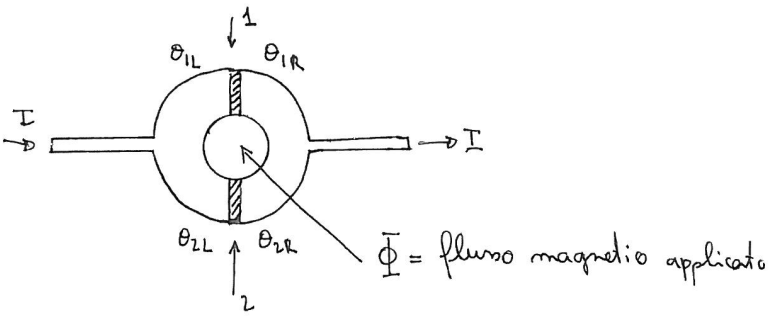
\includegraphics[width=0.6\linewidth]{Immagini - Capitolo 2/SQUID.png}
    \caption{diagramma circuitale dello SQUID.}
    \label{fig: SQUID}
\end{figure}

Supponendo che le giunzioni siano perfettamente identiche, cioè che $I_{C_1} = I_{C_2}$, si ha
\begin{equation}
\label{eq: corrente dello SQUID per giunzioni identiche}
    I = I_C[\sin{(\Delta\theta_1)} + \sin{(\Delta\theta_2)}] = 2I_C\cos{\bigg(\frac{\Delta\theta_1 - \Delta\theta_2}{2}\bigg)}\sin{\bigg(\frac{\Delta\theta_1 + \Delta\theta_2}{2}\bigg)}.
\end{equation}
Se le due giunzioni sono perfettamente bilanciate, applicando una corrente $I < I_C$ ci si aspetta una differenza di fase identica, ossia $\Delta\theta_1 = \Delta\theta_2$, con 
\begin{equation}
    \Delta\theta = \sin^{-1}{\bigg(\frac{I}{2I_C}\bigg)} \neq 0.
\end{equation}
Tuttavia, questo è vero solo se non è presente un campo magnetico all'interno dell'anello. In questo caso la differenza $\Delta\theta_1 - \Delta\theta_2$ dipende dal flusso magnetico $\Phi$ attraverso il dispositivo. Per determinare questa quantità si procede in modo analogo a quanto fatto per la quantizzazione del flusso di campo magnetico per un superconduttore toroidale. Si considerano quindi due cammini $L_1$ ed $L_2$ all'interno del superconduttore dove $\vB = \vo$ e $\vJ_S = \vo$, come mostrato in figura \ref{fig: SQUID calcolo}. 
\begin{equation}
    \begin{cases}
        \theta_{1,R} - \theta_{2,R} = \dfrac{2e}{\hbar}\displaystyle\int_{L_1}\vA \cdot d\vl \\
        \theta_{2,L} - \theta_{1,L} = \dfrac{2e}{\hbar}\displaystyle\int_{L_2}\vA \cdot d\vl
    \end{cases},
\end{equation}
la cui somma risulta in
\begin{equation}
\label{eq: differenza di fase dello SQUID}
    \begin{split}
        \theta_{1,R} - \theta_{2,R} + \theta_{1,L} - \theta_{2,L} &= \frac{2e}{\hbar}\oint\vA \cdot d\vl \\
        \Delta\theta_1 - \Delta\theta_2 &= \frac{2e}{\hbar}\Phi \\
        &= \frac{2\pi\Phi}{\Phi_0}.
    \end{split}
\end{equation}
\begin{figure}[h]
    \centering
    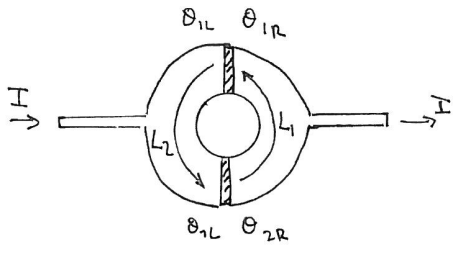
\includegraphics[width=0.5\linewidth]{Immagini - Capitolo 2/SQUID calcolo.png}
    \caption{scelta dei due percorsi per il calcolo della corrente nello SQUID.}
    \label{fig: SQUID calcolo}
\end{figure}

Sostituendo quanto trovato in \eqref{eq: differenza di fase dello SQUID} nell'equazione della corrente \eqref{eq: corrente dello SQUID per giunzioni identiche} si ha
\begin{equation}
    I = 2I_C\sin{\bigg(\frac{\Delta\theta_1 + \Delta\theta_2}{2}\bigg)}\cos{\bigg(\frac{\pi\Phi}{\Phi_0}\bigg)},
\end{equation}
per cui la corrente critica è
\begin{equation}
    I_C(\Phi) = 2I_C\bigg|\cos{\bigg(\frac{\pi\Phi}{\Phi_0}\bigg)}\bigg|.
\end{equation}
L'andamento della corrente critica $I_C(\Phi)$ è mostrato in figura \ref{fig: IC SQUID.png}. Si noti che per $I_C = 0$, una piccolissima corrente $I$ genera una differenza di potenziale ai capi della giunzione. Questo dispositivo permette di misurare piccolissime variazioni di flusso del campo magnetico, con precisione fino a variazioni del campo magnetico nell'ordine di $\SI{e-10}{\tesla}$ attraverso la misura di differenza di potenziale ai capi delle giunzioni quando $I_C \simeq 0$ e $I_C \neq 0$.
\begin{figure}[h]
    \centering
    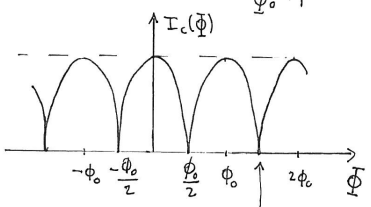
\includegraphics[width=0.5\linewidth]{Immagini - Capitolo 2/IC SQUID.png}
    \caption{andamento della corrente critica $I_C(\Phi)$ dello SQUID.}
    \label{fig: IC SQUID.png}
\end{figure}

\section{Modello di Cooper}
Nonostante il modello di Landau e Ginzburg nonostante sia una teoria fenomenologica che descrive con grande successo molti aspetti e proprietà dei superconduttori, il grande limite di questa teoria tuttavia è la mancata spiegazione dell'origine microscopica del fenomeno di superconduttività. A completare e generalizzare la teoria di Landau e Ginzburg furono Bardeen, Cooper e Schiffer con la loro teoria BCS che provvedeva una spiegazione della superconduttività a livello microscopico prevedendo quantitativamente molte delle proprietà dei superconduttori ``classici''.

Un anno prima della pubblicazione della teoria BCS, Cooper dimostrò che lo stato fondamentale normale di un gas di elettroni è instabile rispetto alla formazione di ``stati legati'' di coppie di elettroni, dove la coppia non è legata nel modo usuale ma lo è a causa delle presenza di un ``mare'' di Fermi, l'elemento chiave per l'esistenza di questo stato; inoltre, in realtà tale stato è a molti elettroni. Alla temperatura $T = \SI{0}{\kelvin}$, nello stato fondamentale normale, tutti gli orbitali macroscopici degli elettroni in un metallo sono occupati fino a $E < \epsilon_F$, mentre i restanti sono vuoti. L'idea di Cooper è di considerare un mare di Fermi ``congelato'' più una coppia di elettroni con energia $E > \epsilon_F$ e con un potenziale efficace a due corpi attrattivo $U(\vr_1,\vr_2) < 0$. Cooper immaginava quindi un'interazione molto debole tra gli elettroni con $U(\vr_1,\vr_2) \simeq 0$; in queste condizioni ci si aspetterebbe che l'eccesso di energia cinetica $\Delta E_K = (E_{K_1} + E_{K_2} -2\epsilon_F) > 0$ non possa essere compensato dalla diminuzione di energia potenziale $\Delta U = 0$. 

Per capire se questo è il caso, si parte dall'equazione di Schr\"odinger corrispondente
\begin{equation}
\label{eq: equazione di Schrodinger BCS completa}
    \bigg[-\frac{\hbar^2}{2m}(\nabla^2_1 + \nabla_2^2) + U(\vr_1,\vr_2)\bigg]\psi(\vr_1,\vr_2) = (\Delta E + 2\epsilon_F)\psi(\vr_1,\vr_2).
\end{equation}
La parte della funzione d'onda $\psi(\vr_1,\vr_2)$ legata allo spin può essere o nello stato di singoletto o in quello di tripletto; tuttavia, maggior parte dei superconduttori le coppie di Cooper corrispondono a stati di singoletto
\begin{equation}
    \chi_{\sigma_1,\sigma_2} = \frac{1}{\sqrt{2}}(\ket{\upa\doa} - \ket{\doa\upa}),
\end{equation}
la quale è antisimmetrica per lo scambio degli elettroni, ossia degli indici $1 \leftrightarrow 2$, mentre $\psi(\vr_1,\vr_2)$ è simmetrica dato che le particelle in questione sono appunto identiche. L'autovalore $\Delta E$ è definito relativamente al livello di Fermi $2\epsilon_F$. Si consideri il sistema di coordinate del centro di massa
\begin{equation}
    \begin{cases}
        \vR = \dfrac{1}{2}(\vr_1 + \vr_2) \\
        \vr = \vr_1 - \vr_2
    \end{cases},
\end{equation}
così da riscrivere l'equazione di Schr\"odinger come
\begin{equation}
   \bigg[-\frac{\hbar^2}{4m}\nabla^2_R - \frac{2\hbar^2}{2m}\nabla^2_r\bigg]\psi(\vR,\vr) + U(\vr)\psi(\vR,\vr) = (\Delta E + 2\epsilon_F)\psi(\vR,\vr).
\end{equation}
Separando adesso la funzione d'onda nelle sue variabili ponendo
\begin{equation}
    \psi(\vR,\vr) = \Phi(\vR)\psi(\vr),\quad \Phi(\vR) = e^{i(\vQ\cdot \vR)}
\end{equation}
e considerando al momento solo lo stato con $\vQ = \vo$, si rimane con
\begin{equation}
\label{eq: equazione di Schrodinger BCS psi(r)}
   \bigg[- \frac{2\hbar^2}{2m}\nabla^2_r + U(\vr)\bigg]\psi(\vr) = (\Delta E + 2\epsilon_F)\psi(\vr),
\end{equation}
gli stati con $\vQ \neq \vo$ sono invece necessari per descrivere un flusso di corrente stazionario. Si supponga adesso che la funzione d'onda $\psi(\vr)$ sia una certa sovrapposizione su tutti gli stati
\begin{equation}
    \psi(\vr) = \frac{1}{\sqrt{V}}\sum_{k  > k_F}a_ke^{i(\vk \cdot \vr)},
\end{equation}
dove la somma è fatta su tutti i numeri d'onda $k \equiv |\vk| > k_F$. Sostituendo quest'ultima relazione nell'equazione \eqref{eq: equazione di Schrodinger BCS psi(r)} si ha
\begin{equation}
    \sum_{k > k_F}[2(\epsilon_k - \epsilon_F) - \Delta E]a_ke^{i(\vk \cdot \vr)} + \sum_{k > k_F}U(\vr)a_ke^{i(\vk \cdot \vr)} = 0,\quad \epsilon_k \equiv \frac{\hbar^2k^2}{2m}
\end{equation}
che se moltiplicata per $e^{-i(\vk' \cdot \vr)}/V$ ed integrata su $\vr$ porta a
\begin{equation}
    \begin{split}
        0 &= [2(\epsilon_{k'} - \epsilon_F) - \Delta E]a_{k'} + \sum_{k > k_F}a_k\int\frac{d^3r}{V}U(\vr)e^{i(\vk - \vk')\cdot \vr} \\
        &= [2(\epsilon_{k'} - \epsilon_F) - \Delta E]a_{k'} + \sum_{k > k_F}a_kU(\vk,\vk'),
    \end{split}
\end{equation}
dove $U(\vk,\vk')$ è la trasformata di Fourier di $U(\vr)$, ossia
\begin{equation}
    U(\vk,\vk') = \frac{1}{V}\int d^3r\,e^{i(\vk - \vk')\cdot \vr}U(\vr).
\end{equation}
Per procedere si deve necessariamente supporre la forma del potenziale di interazione, in questo caso
\begin{equation}
    U(\vk,\vk') =
    \begin{cases}
        -V_0,\quad 0 \le \epsilon_{k,k'} - \epsilon_F \le \hbar\omega_D\\
        0,\quad \mathrm{altrimenti}
    \end{cases},
\end{equation}
dove $\hbar\omega_D$ è un valore di soglia che formalizza l'assunzione che solo gli elettroni in una banda attorno al livello di Fermi contribuiscono al processo di scattering $(\vk_i,\vk'_i) \to (\vk_f,\vk'_f)$, il quale è possibile solo se $|\vk_i|$, $|\vk_i'|$, $|\vk_f|$ e $|\vk_f'|$ sono maggiori di $k_F$. In particolare, $\hbar\omega_D$ è l'energia di Debye, ossia la massima energia che può acquisire un fonone in un reticolo. Questo riflette l'idea che l'interazione tra elettroni avvenga attraverso lo scambio di fononi reticolari. Si trova allora
\begin{equation}
    \sum_{k > k_F}a_kU(\vk,\vk') = 
    \begin{cases}
        -V_0\nsump{k > k_F}a_k,\quad 0 \le \epsilon_{k'} - \epsilon_F \le \hbar\omega \\
        0,\quad \mathrm{altrimenti}
    \end{cases},
\end{equation}
quindi si ha
\begin{align}
    [2(\epsilon_{k'} - \epsilon_F) - \Delta E]a_{k'} - V_0\sump_{k > k_F}a_k &= 0 \\
    a_{k'} &= \frac{V_0\nsump{k > k_F}a_k}{2(\epsilon_{k'} - \epsilon_F) - \Delta E},
\end{align}
da cui, sommando su $k'$, si trova
\begin{equation}
    \frac{1}{V_0} = \sump_{k > k_F}\frac{1}{2(\epsilon_k - \epsilon_F) - \Delta E}.
\end{equation}
La somma può essere trasformata in un integrale se si introduce la densità degli stati $D(\epsilon_k)$, così da avere
\begin{equation}
    \int_{\epsilon_F}^{\epsilon_F + \hbar\omega_D}d\epsilon\,\frac{V_0D(\epsilon)}{2(\epsilon - \epsilon_F) - \Delta E} = 1.
\end{equation}
Considerando adesso il limite in cui $\hbar\omega_D \ll 1$, allora $D(\epsilon) \simeq D(\epsilon_F)$ e l'integrale si riduce all'equazione
\begin{equation}
    \begin{split}
        \frac{V_0}{2}D(\epsilon_F)\log{[2(\epsilon - \epsilon   _F) - \Delta E]}|_{\epsilon_F}^{\epsilon_F + \hbar\omega_D} &= \frac{V_0}{2}D(\epsilon_F)\log{\bigg(\frac{\Delta E - 2\hbar\omega_D}{\Delta E}\bigg)} \\
        &\simeq 1,
    \end{split}
\end{equation}
che risolvendo per $\Delta E$ restituisce
\begin{equation}
\label{eq: differenza di energia stati BCS}
    \Delta E = -\frac{2\hbar\omega_D}{e^{2/V_0D(\epsilon_F)} - 1}.
\end{equation}
In particolare, nel limite di interazione debole $V_0D(\epsilon_F) \ll 1$, l'esponenziale domina a denominatore risultando in 
\begin{equation}
\label{eq: differenza di energia stati BCS limite interazione debole}
    \Delta E \simeq -2\hbar\omega_De^{-2/V_0D(\epsilon_F)},
\end{equation}
che se sostituito in $\Delta E + 2\epsilon_F$ porta al risultato ottenuto da Cooper
\begin{equation}
    \Delta E + 2\epsilon_F \simeq 2\epsilon_F - 2\hbar\omega_De^{-2/V_0D(\epsilon_F)} < 2\epsilon_F.
\end{equation}
Esiste quindi uno stato ``legato'' con energia negativa, rispetto alla superficie di Fermi costituito da elettroni con $|\vk| > k_F$, cioè con energia cinetica superiore a $\epsilon_F$. Lo stato composto da elettroni accoppiati in questo modo avrà sempre un'energia minore di quella dello stato fondamentale, anche per valori di $V_0$ arbitrariamente piccoli. Questo è il motivo per cui si considera lo stato fondamentale normale instabile rispetto alla formazione di coppie di Cooper. Inoltre, questo risultato non può essere ottenuto con metodi perturbativi sviluppando in potenze di $V_0$. L'espressione ottenuta per $\Delta E$ nell'equazione \eqref{eq: differenza di energia stati BCS limite interazione debole} mette in evidenza una gerarchia di energia $\epsilon_F \gg \hbar\omega_D \gg |\Delta E|$, assumendo poi che $|\Delta E| \simeq kT_c$, allora tale gerarchia spiega come mai la transizione a superconduttore avviene a temperature molto basse rispetto alla temperatura di Debye $T_D = \hbar\omega_D/k$. 

\paragraph{Effetto isotropico.} L'idea che 
l'attrazione tra elettroni sia conseguenza dell'interazione elettrone-fonone è confermata dall'effetto isotropico, che consiste nella relazione $T_c \propto m^{-\alpha}$, dove $m$ è la massa dello ione che costituisce, il reticolo cristallino. La teoria delle vibrazioni nei cristalli prevede che la frequenza di vibrazione $\omega(q)$ siano tutte proporzionali a $\sqrt{K/m}$, dove $K$ è la costante elastica del potenziale classico di interazione elastica fra tutti i primi vicini del reticolo. Quindi, poiché
\begin{equation}
    kT_c \simeq \Delta E \propto \hbar\omega_D \propto \sqrt{\frac{K}{m}},
\end{equation}
si trova immediatamente che $T_c \propto m^{-1/2}$, che corrisponde al valore osservato dell'esponente critico per i metalli puri. L'ipotesi che le interazioni elettrone-nucleo fossero importanti è dovuta a Fr\"olich: al passaggio di un elettrone. il reticolo tende a deformarsi creando un eccesso di carica totale che può attrarre un secondo elettrone, come mostrato in figura \ref{fig: carica di un reticolo}. In particolare, gli elettroni interagiscono a distanza attraverso il reticolo e tale interazione è attrattiva e mediata dallo scambio di fononi. Nei superconduttori ad alta temperatura l'effetto isotropico non si verifica, ciò potrebbe indicare che non sono i fononi i responsabili del gap di energia.
\begin{figure}[h]
    \centering
    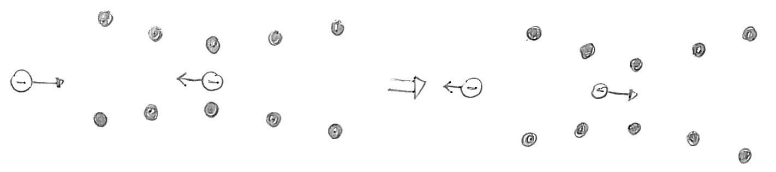
\includegraphics[width=0.6\linewidth]{Immagini - Capitolo 2/carica di un reticolo.png}
    \caption{deformazione della distribuzione di carica di un reticolo cristallino al passaggio di un elettrone.}
    \label{fig: carica di un reticolo}
\end{figure}

\subsection{Stato fondamentale}
Più sopra si è dimostrato che il mare di Fermi è instabile per la creazione di coppie di Cooper quando l'interazione effettiva tra due elettroni è attrattiva. Ci si aspetta di conseguenza una condensazione di coppie di Cooper fino a quando non si raggiunge uno stato di equilibrio. Questo avviene dopo che lo stato di Fermi è cambiato così tanto che l'aggiunta di un'altra coppia di Cooper non è più associata ad una diminuzione dell'energia. Per studiare uno stato interagente di questo tipo si deve introdurre il formalismo della seconda quantizzazione per i fermioni seguendo un procedimento del tutto simile al caso bosonico, con la differenza che questa volta si introduce una relazione di anti-commutazione
\begin{equation}
    \acomm{\hata}{\hatb} = \hata\hatb + \hatb\hata,
\end{equation}
passando così dalla statistica di Bose-Einstein a quella di Fermi-Dirac. Fin dal principio è conveniente lavorare nello spazio degli impulsi introducendo gli operatori di creazione $\hatC^\dg_{k\sigma}$ e di distruzione $\hatC_{k\sigma}$ che, rispettivamente, creano e distruggono un fermione con momento $\vk$ e terza componente di spin $\sigma = \{\upa,\doa\}$. Indicando con $\kO$ lo stato di vuoto corrispondente alla totale assenza di fermioni in modo tale che $\hatC_{k\sigma}\kO = 0$, gli operatori $\hatC$ e $\hatC^\dg$ soddisfano le seguenti regole di anticommutazione
\begin{equation}
    \begin{cases}
        \acomm{\hatC_{k\sigma}^\dg}{\hatC_{k'\sigma'}} = \delta_{k,k'}\delta_{\sigma,\sigma'} \\
        \acomm{\hatC_{k\sigma}^\dg}{\hatC^\dg_{k'\sigma'}} = 0 \\
        \acomm{\hatC_{k\sigma}}{\hatC_{k'\sigma'}} = 0
    \end{cases}.
\end{equation}
Applicando l'operatore di creazione $\hatC^\dg$ sullo stato fondamentale $\kO$ si ottiene uno stato 
\begin{equation}
    \hatC^\dg_{k\sigma}\kO = \ket{k\sigma} \equiv \ket{1_{k\sigma}},
\end{equation}
inoltre gli stati a molti elettroni sono automaticamente antisimmetrici per lo scambio delle particelle. Se poi $(k,\sigma) = (k',\sigma')$, allora $\ket{2_{k\sigma}} = -\ket{2_{k\sigma}}$, per cui $\ket{2_{k\sigma}} = 0$, o analogamente
\begin{equation}
    (\hatC^\dg_{k\sigma})^2 = (\hatC_{k\sigma})^2 = 0,
\end{equation}
che corrisponde al principio di esclusione di Pauli in Meccanica quantistica. L'operatore $\hatN_{k\sigma} = \hatC^\dg_{k\sigma}\hatC_{k\sigma}$ è l'operatore ``numero di elettroni'' con impulso $\vk$ e terza componente di spin $\sigma$, il quale soddisfa le seguenti regole di commutazione
\begin{equation}
    \begin{cases}
        \comm{\hatN_{k\sigma}}{\hatC^\dg_{k\sigma}} = \hatC^\dg_{k\sigma}(\hatN_{k\sigma} + 1) \\
        \comm{\hatN_{k\sigma}}{\hatC_{k\sigma}} = \hatC_{k\sigma}(\hatN_{k\sigma} - 1)
    \end{cases}
\end{equation}
e che agisce su uno stato generico $\ket{S}$ come
\begin{equation}
    \hatN_{k\sigma}\ket{S} = 
    \begin{cases}
        0,\quad \ket{S} = \ket{\dots,0_{k\sigma},\dots} \\
        1,\quad \ket{S} = \ket{\dots,1_{k\sigma},\dots}
    \end{cases},
\end{equation}
da cui si deduce anche che $(\hatN_{k\sigma})^2 = \hatN_{k\sigma}$. L'operatore ``numero totale'' di elettroni è dato da
\begin{equation}
    \hatN = \nsum_{k\sigma}\hatN_{k\sigma}.
\end{equation}
\begin{obs}
    In Meccanica quantistica non-relativistica per fermioni, il formalismo della seconda quantizzazione permette di evitare l'introduzione degli ingombranti determinanti di Slater. A fissato numero di particelle i approcci sono perfettamente equivalenti.
\end{obs}
Si introduce adesso la funzione d'onda per la coppia di Cooper come
\begin{equation}
    \psi_{CP} \equiv \psi_\sigma\psi_r = \frac{1}{\sqrt{2}}(\ket{\upa\doa} - \ket{\doa\upa})\psi(\vr_1,\vr_2),
\end{equation}
dove
\begin{equation}
    \psi(\vr_1,\vr_2) = N\sum_{k > k_F}a_ke^{i\vk\cdot(\vr_1 - \vr_2)}.
\end{equation}
Nello spazio degli impulsi con il formalismo della seconda quantizzazione si può scrivere
\begin{equation}
    N\sum_{k > k_F}a_k\ket{1_{k\upa},1_{-k\doa}}_F = N\sum_{k > k_F}a_k\hatC^\dg_{k\upa}\hatC_{-k\doa}\ket{F}.
\end{equation}
Pertanto, conviene introdurre l'operatore di creazione di coppie di Cooper come
\begin{equation}
    \hatP^\dg_k = \hatC^\dg_{k\upa}\hatC^\dg_{-k\doa},\quad \hatP_k = \hatC_{-k\doa}\hatC_{k\upa}.
\end{equation}
Sebbene siano operatori composti da due operatori di tipo fermionico non sono totalmente equivalenti
ad operatori bosonici; valgono infatti le seguenti proprietà di commutazione:
\begin{enumerate}
    \item $\comm{\hatP_k^\dg}{\hatP^\dg_{k'}} = \comm{\hatP_k}{\hatP_{k'}} = 0$;
    \item $(\hatP_k^\dg)^2 = 0$;
    \item usando le espressioni degli operatori di creazione e distruzione fermionici $\hatC_{k\upa}\hatC^\dg_{k\upa} = 1 - \hatC_{k\upa}^\dg\hatC_{k\upa}$ e $\hatC^\dg_{-k\doa}\hatC_{-k\doa} = 1 - \hatC_{-k\doa}\hatC^\dg_{-k\doa}$ si ha
    \begin{equation}
        \begin{split}
            \comm{\hatP_k}{\hatP^\dg_k} &= \hatP_k\hatPT_k - \hatPT_k\hatP_k \\
            &= \hatCT_{-k\doa}\hatC_{k\upa}\hatCT_{k\upa}\hatCT_{-k\doa} - \hatCT_{k\upa}\hatCT_{-k\doa}\hatC_{-k\doa}\hatC_{k\upa} \\ 
            &= (1 - \hatN_{-k\doa} - \hatN_{k\upa}).
        \end{split}
    \end{equation}
\end{enumerate}
Pertanto, gli operatori $\hatP_k$ e $\hatP_k^\dg$ non sono operatori canonicamente commutanti, dato che il loro commutatore è diverso da 1.

Si costruisce adesso lo stato fondamentale $\ket{\psi_{BCS}}$ che descrive il superconduttore a $T = \SI{0}{\kelvin}$ in presenza di un condensato di coppie di Cooper. In analogia con i condensati di Bose-Einstein, Schreiffer propose come stato fondamentale lo stato ``coerente'' definito da
\begin{equation}
    \ket{\psi_{BCS}} = \bar{N}\nprod_k e^{\alpha_k\hatP_k^\dg}\kO,\quad \bar{N},\alpha_k \in \C,
\end{equation}
dove $\alpha_k = \alpha_{-k}$ per ogni $k$ e dove $\bar{N}$ è una costante di normalizzazione. Per il principio di esclusione di Pauli, corrispondente a $(\hatPT_k)^2 = 0$, lo stato coerente appena definito si può espandere come
\begin{equation}
    \ket{\psi_{BCS}} = \bar{N}\nprod_k(1 + \alpha_k\hatP_k^\dg)\kO,
\end{equation}
con i parametri $\{\alpha_k\}$ da fissare per minimizzare l'energia dell'hamiltoniana del modello BCS. Per determinare la costante di normalizzazione $\bar{N}$, sapendo che $\mybraket{\Omega}{\Omega} = 1$, si impone la condizione di normalizzazione $\mybraket{\psi_{BCS}}{\psi_{BCS}} = 1$ che porta a
\begin{equation}
    \begin{split}
        1 &= |\bar{N}|^2\prod_{k,k'}\mybrakett{\Omega}{(1 + \alpha_k^*\hatP_k)(1 + \alpha_{k'}\hatP_{k'}^\dg)}{\Omega} \\
        &= |\bar{N}|^2\prod_{k,k'}(\mybraket{\Omega}{\Omega} + \mybrakett{\Omega}{\alpha_k^*\alpha_{k'}\hatP_k\hatP_{k'}^\dg}{\Omega}) \\
        &= |\bar{N}|^2\prod_{k,k'}(1 + \alpha_k^*\alpha_{k'}\mybrakett{\Omega}{\hatP_k\hatP_{k'}^\dg}{\Omega}) \\
        &= |\bar{N}|^2\nprod_{k}\mybrakett{\Omega}{(1 + \alpha_k^*\hatP_k)(1 + \alpha_k\hatP_k^\dg)}{\Omega} \\
        &= |\bar{N}|^2\nprod_{k}\mybrakett{\Omega}{(1 + |\alpha_k|^2(1 - \hatN_{-k\doa} - \hatN_{k\upa} + \hatP_k^\dg\hatP_k)}{\Omega} \\
        &= |\bar{N}|^2\nprod_{k}(1 + |\alpha_k|^2),
    \end{split}
\end{equation}
da cui si ricava
\begin{equation}
    \bar{N} = \nprod_k\frac{1}{\sqrt{1 + |\alpha_k|^2}},
\end{equation}
dove si sono usate le proprietà degli operatori di creazione e distruzione di coppie di Cooper $\mybrakett{\Omega}{\hatP_{k}\hatP_{k'}^\dg}{\Omega} = \delta_{k,k'}$ e $\mybrakett{\Omega}{\hatP_k}{\Omega} = \mybrakett{\Omega}{\hatP_k^\dg}{\Omega} = 0$. Dunque, lo stato fondamentale è
\begin{equation}
    \ket{\psi_{BCS}} = \nprod_k\bigg(\frac{e^{i\theta_k}}{\sqrt{1 + |\alpha_k|^2}} + \frac{\alpha_ke^{i\theta_k}}{\sqrt{1 + |\alpha_k|^2}}\hatP_k^\dg\bigg)\kO \equiv \nprod_k(u_k^* + v_k^*\hatP_k^\dg)\kO,
\end{equation}
dove si ha una possibile fase globale data da $|u_k|^2 + |v_k|^2 = 1$ con $|u_k|^2 = |u_{-k}|^2$ e $|v_k|^2 = |v_{-k}|^2$. Usando poi il fatto che $\hatP_k\hatP_k^\dg\kO = \kO$, si può riscrivere lo stato fondamentale in termini del livello di Fermi come
\begin{equation}
    \begin{split}
        \ket{\psi_{BCS}} &= \nprod_k(u_k^* + v_k^*\hatP_k^\dg)\prod_{k < k_F}\hatP_k\hatP_k^\dg\kO \\
        &= \nprod_k(u_k^* + v_k^*\hatP_k^\dg)\prod_{k < k_F}\hatP_k\ket{F} \\
        &= \prod_{k > k_F}(u_k^* + v_k^*\hatP_k^\dg)\prod_{k < k_F}[(u_k^* + v_k^*\hatP_k^\dg)\hatP_k]\ket{F} \\
        &= \prod_{k > k_F}(u_k^* + v_k^*\hatP_k^\dg)\prod_{k < k_F}(u_k^*\hatP_k + v_k^*)\ket{F},
    \end{split}
\end{equation}
dove il primo termine restituisce il numero di coppie di Cooper, mentre il secondo il numero di lacune di Cooper. L'andamento del numero di fermioni con momento $\vk$ e terza componente di spin $\sigma$ è mostrato in figura \ref{fig: numero fermioni BCS}.
\begin{figure}[h]
    \centering
    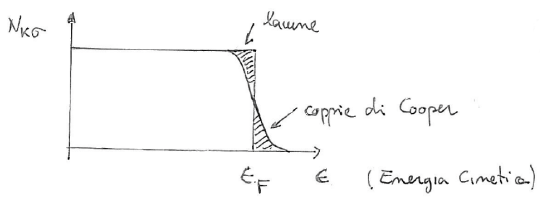
\includegraphics[width=0.6\linewidth]{Immagini - Capitolo 2/numero fermioni BCS.png}
    \caption{andamento del numero di fermioni nel superconduttore in funzione dell'energia cinetica $\epsilon$.}
    \label{fig: numero fermioni BCS}
\end{figure}

Il prossimo passo è quello di introdurre l'hamiltoniana del modello BCS. L'hamiltoniana di partenza ha la stessa forma di quella di Gross-Pitaevskii con potenziale di interazione a delta di Dirac per descrivere i gas diluiti a bassa temperatura, con la differenza che ora si devono considerare gli operatori fermionici, per cui 
\begin{equation}
    \hatH_{BCS} = \sump_{k,\sigma}\epsilon_k\hatC^\dg_{k\sigma}\hatC_{k\sigma} - |g|\sump_{\substack{k_1,k_2 \\ \sigma_1,\sigma_2 \\
    q}}\hatC^\dg_{k_1 + q,\sigma_1}\hatC^\dg_{k_2 - q,\sigma_2}\hatC_{k_1\sigma_1}\hatC_{k_2\sigma_2},
\end{equation}
dove l'indice della somma $\Sigma'$ è ristretto a $\epsilon_F - \hbar\omega_D \le \epsilon_k \le \epsilon_F + \hbar\omega_D$. Se ora si assume che l'interazione rilevante per la superconduttività coinvolga solo le coppie di Cooper, l'hamiltoniana diventa
\begin{equation}
    \hatH_{BCS} = \sump_{k,\sigma}\epsilon_k\hatN_{k\sigma} - |g|\sump_{k,k'}\hatP^\dg_k\hatP_{k'},\quad \epsilon_k = \frac{\hbar^2k^2}{2m}.
\end{equation}
Tuttavia, questa hamiltoniana non può essere diagonalizzata in modo esatto. Pertanto, si deve usare il fatto che la funzione d'onda $\ket{\psi_{BCS}}$ contiene i parametri $u_k^*$ e $v_k^*$ che possono essere trattati con il metodo variazionale, i quali vengono fissati richiedendo che $E = \mybrakett{\psi_{BCS}}{\hatH}{\psi_{BCS}}$ sia minima con il vincolo che $N \equiv \mybrakett{\psi_{BCS}}{\hatN}{\psi_{BCS}}$ sia fissato e valga la condizione $|u_k|^2 + |v_k|^2 = 1$. Si considera in primis il termine cinetico
\begin{equation}
    \hatT \equiv \sump_{k,\sigma}\epsilon_k\hatN_{k\sigma} = \sump_{k,\sigma}\epsilon_k(\hatN_{k\upa} + \hatN_{-k\doa}).
\end{equation}
Sapendo che $\hatN^\dg_{k\upa} = \hatN_{k\upa}$, si calcola
\begin{equation}
    \begin{split}
        \vmedio{\hatN_{k\upa}}_{BCS} = \vmedio{\hatC^\dg_{k\upa}\hatC_{k\upa}}_{BCS} &= \mybrakett{\Omega}{(u_k + v_k\hatP_k)\hatN_{k\upa}(u_k^* + v_k^*\hatP_k^\dg)}{\Omega} \\
        &= |u_k|^2\cancelto{0}{\mybrakett{\Omega}{\hatN_{k\upa}}{\Omega}} + |v_k|^2\mybrakett{\Omega}{\hatP_k\hatN_{k\upa}\hatPT_k}{\Omega} \\
        &= |v_k|^2\mybrakett{\Omega}{\hatP_k\hatN_{k\upa}\hatP_k^\dg}{\Omega} \\
        &= |v_k|^2,
    \end{split}
\end{equation}
dove si è usata la proprietà $\comm{\hatN_{k\upa}}{\hatP_k^\dg} = \hatP_k^\dg$. In modo simile, si può ricavare $\vmedio{\hatN_{-k\doa}}_{BCS} = |v_k|^2$. Dunque, il valor medio $N$ è dato da
\begin{equation}
    N \equiv \mybrakett{\psi_{BCS}}{\hatN_{k\sigma}}{\psi_{BCS}} = 2\nsump{k}|v_k|^2 = \nsump{k}(|v_k|^2 - |u_k^2| + 1),
\end{equation}
per cui 
\begin{equation}
    \bigvmedio{\sump_{k,\sigma}\epsilon_k\hatC^\dg_{k\sigma}\hatC_{k\sigma}}_{BCS} = 2\nsump{k}\epsilon_k|v_k|^2 = \nsump{k}\epsilon_k(|v_k|^2 - |u_k^2| + 1).
\end{equation}
Per quanto riguarda la parte di interazione 
\begin{equation}
    \begin{split}
        \vmedio{\hatPT_k\hatP_{k'}}_{BCS} &= \mybrakett{\Omega}{(u_{k'} + v_{k'}\hatP_{k'})(u_k + v_k\hatP_k)(\hatPT_k\hatP_{k'}) \\ 
        &\times (u^*_{k'} + v^*_{k'}\hatPT_{k'})(u^*_k + v_k^*\hatPT_k)}{\Omega} \\
        &= \mybrakett{\Omega}{\hatP_k\hatPT_k\hatP_{k'}\hatPT_{k'}}{\Omega}v_kv_{k'}^*u_{k'}u_k^* \\
        &= v_kv_{k'}^*u_{k'}u_k^*.
    \end{split}
\end{equation}
Quindi, il valore medio dell'hamiltoniana espresso in funzione dei parametri $v_k$ e $u_k$ è
\begin{equation}
    \begin{split}
        \vmedio{\hatH}_{BCS} \equiv E &= 2\nsump{k}\epsilon_k|v_k|^2 - |g|\sump_{k,k'}v_kv_{k'}^*u_{k'}u_k^* \\
        &= \nsump{k}\epsilon_k(|v_k|^2 - |u_k|^2 + 1) - |g|\sump_{k,k'}v_kv_{k'}u_{k'}u_k^*.
    \end{split}
\end{equation}
Le condizioni di minimo sono
\begin{equation}
    \begin{cases}
        \dfrac{\p}{\p u_k^*}\bigg[E - \mu N + \nsump{k}E_k(|u_k|^2 + |v_k|^2 - 1)\bigg] = 0 \\[2ex]
        \dfrac{\p}{\p v_k^*}\bigg[E - \mu N + \nsump{k}E_k(|u_k|^2 + |v_k|^2 - 1)\bigg] = 0
    \end{cases},
\end{equation}
dove $\mu$ è il moltiplicatore di Lagrange di $N$, mentre $E_k$ è quello dei vincoli $|u_k|^2 + |v_k|^2 = 1$. Quindi, ponendo $\Sigma \equiv E_k(|u_k|^2 + |v_k|^2 - 1)$, computando i vari termini nella prima equazione del sistema
\begin{equation}
    \mu\frac{\p N}{\p u_k^*} = -\mu u_k, \quad \frac{\p \Sigma}{\p u_k^*} = E_ku_k,\quad \frac{\p E}{\p u_k^*} = -\epsilon_ku_k - |g|v_k\nsump{k'}v_{k'}^*u_{k'}
\end{equation}
e per la seconda equazione del sistema
\begin{equation}
    \mu\frac{\p N}{\p v_k^*} = \mu v_k, \quad \frac{\p \Sigma}{\p v_k^*} = E_kv_k,\quad \frac{\p E}{\p v_k^*} = -\epsilon_kv_k - |g|u_k\nsump{k'}v_{k'}u_{k'}^*,
\end{equation}
si ottiene
\begin{equation}
    \begin{cases}
        (\epsilon_k - \mu)u_k + \Delta v_k = E_ku_k \\
        \Delta^*u_k - (\epsilon_k - \mu)v_k = E_kv_k
    \end{cases},
\end{equation}
dove si sono introdotti i parametri di gap
\begin{equation}
\label{eq: parametri di gap BCS definizione}
    \Delta \equiv |g|\nsump{k}v_k^*u_k,\quad \Delta^* \equiv |g|\nsump{k}v_ku_k^*.
\end{equation}
Nella teoria BCS, il parametro $\Delta$ ha un importante significato fisico; infatti, considerando il valore medio dell'operatore $\hatP_k$ sullo stato fondamentale 
\begin{equation}
    \begin{split}
        \vmedio{\hatP_k}_{BCS} &= \mybrakett{\Omega}{(u_k + v_k\hatP_k)\hatP_k(u_k^* + v_k^*\hatPT_k)}{\Omega} \\
        &= u_kv_k^*\mybrakett{\Omega}{\hatP_k\hatPT_k}{\Omega} \\
        &= u_kv_k^*
    \end{split}
\end{equation}
si trova che 
\begin{equation}
    \Delta = |g|\nsump{k}\vmedio{\hatP_k}_{BCS},
\end{equation}
ossia il parametro $\Delta$ è legato al valore di aspettazione delle coppie di Cooper sullo stato fondamentale $\ket{\psi_{BCS}}$. Per trovare $\Delta$ bisogna risolvere il sistema lineare
\begin{equation}
    \begin{pmatrix}
        \epsilon_k - \mu & \Delta \\
        \Delta^* & -\epsilon_k + \mu
    \end{pmatrix}
    \begin{pmatrix}
        u_k \\
        v_k
    \end{pmatrix} \equiv M(\Delta)
    \begin{pmatrix}
        u_k \\
        v_k
    \end{pmatrix} = E_k
    \begin{pmatrix}
        u_k \\
        v_k
    \end{pmatrix},
\end{equation}
il quale ha soluzione non banale se e solo se 
\begin{equation}
    \det{[M(\Delta) - \MI E_k]} = \det
    \begin{pmatrix}
        \epsilon_k - \mu - E_k & \Delta \\
        \Delta^* & -\epsilon_k + \mu - E_k
    \end{pmatrix} = 0,
\end{equation}
la quale porta all'equazione di secondo grado $E_k^2 - (\epsilon_k - \mu)^2 - |\Delta|^2 = 0$, da cui a sua volta si trovano gli autovalori 
\begin{equation}
    \begin{cases}
        E_k = \sqrt{(\epsilon_k - \mu)^2 + |\Delta|^2} \\
        E_k' = -E_k
    \end{cases}.
\end{equation}
Quindi, si nota che $E_k$ corrisponde all'energia di un quasi-elettrone mentre $E_k'$ corrisponde all'energia di una quasi-lacuna. Per trovare ora un'equazione per $\Delta$ si parte dalle equazioni
\begin{equation}
    \begin{cases}
        v_k^*[(\epsilon_k - \mu)u_k + \Delta v_k] = E_ku_kv_k^* \\
        u_k[\Delta u_k^* - (\epsilon_k - \mu)v_k^*] = E_kv_k^*u_k
    \end{cases}
\end{equation}
la cui somma porta alla relazione
\begin{equation}
\label{eq: relazione parametro di gap BCS}
    u_kv_k^* = \frac{\Delta}{2E_k}
\end{equation}
ed anche alle relazioni
\begin{equation}
    \begin{cases}
        |v_k|^2 = \dfrac{1}{2}\bigg(1 - \dfrac{\epsilon_k - \mu}{E_k}\bigg) \\[2ex]
        |u_k|^2 = \dfrac{1}{2}\bigg(1 + \dfrac{\epsilon_k - \mu}{E_k}\bigg)
    \end{cases}.
\end{equation}
Considerando per prima la relazione \eqref{eq: relazione parametro di gap BCS} e usando la definizione del parametro di gap introdotta in equazione \eqref{eq: parametri di gap BCS definizione} si ottiene
\begin{equation}
    \frac{|g|}{2}\nsump{k}\frac{1}{[(\epsilon_k - \mu)^2 + |\Delta|^2]^{1/2}} = 1.
\end{equation}
Quest'ultima equazione è centrale nella teoria BCS in quanto determina il parametro di gap $|\Delta|$ a $T = \SI{0}{\kelvin}$. Per valutare questa quantità, si può operare la sostituzione
\begin{equation}
    \nsump{k} \to D(\epsilon_F)\int_{-\hbar\omega_D}^{\hbar\omega_D}d\epsilon = 2D(\epsilon_F)\int_0^{\hbar\omega_D}d\epsilon,\quad \epsilon \equiv \epsilon_k - \mu,
\end{equation}
passando così dal discreto ad un intervallo continuo assumendo che i livelli energetici siano molto densi; in questo modo si ottiene
\begin{equation}
    \Lambda\int_0^{\hbar\omega_D}\frac{d\epsilon}{[\epsilon^2 + |\Delta|^2]^{1/2}} = 1,\quad \Lambda \equiv |g|D(\epsilon_F).
\end{equation}
Per risolvere questo integrale si utilizza la formula generale
\begin{equation}
    \int_0^b \frac{dx}{\sqrt{x^2 + a^2}} = -\frac{1}{2}\log{(a^2)} + \log{(b + \sqrt{a^2 + b^2})},
\end{equation}
che in questo caso restituisce
\begin{equation}
    \begin{split}
        1 &= \Lambda\bigg\{-\frac{1}{2}\log|\Delta|^2 + \log{\bigg[\hbar\omega_D + \sqrt{|\Delta|^2 + (\hbar\omega_D)^2}\bigg]}\bigg\} \\
        &\simeq \Lambda\log{\bigg(\frac{2\hbar\omega_D}{|\Delta|}\bigg)},
    \end{split}
\end{equation}
da cui si ricava finalmente la formula per il parametro di gap a temperatura $T = \SI{0}{\kelvin}$ della teoria BCS
\begin{equation}
\label{eq: formula parametro gap a T=0 BCS}
    |\Delta| \simeq 2\hbar\omega_De^{-1/\Lambda}.
\end{equation}
Si possono anche calcolare gli autovettori della matrice $M(\Delta)$ corrispondenti agli autovalori $E_k$ ed $E_k'$ rispettivamente che risultano essere i vettori $\begin{pmatrix} u_k & -v_k\end{pmatrix}^T$ e $\begin{pmatrix} v_k^* & -u_k^*\end{pmatrix}^T$. Inoltre, dalla relazione \eqref{eq: relazione parametro di gap BCS} si può dedurre che gli autovettori della matrice $M(-\Delta)$ sono $\begin{pmatrix} u_k & -v_k\end{pmatrix}^T$ e $\begin{pmatrix} v_k^* & u_k^*\end{pmatrix}^T$.

\subsection{Stati eccitati}
Avendo ottenuto $\ket{\psi_{BCS}}$ tramite metodi variazionali, il passo successivo è quello di fare predizioni sulle proprietà fisiche dei superconduttori. Il metodo utilizzato per trovare gli stati eccitati è simile a quello usato nei superfluidi attraverso la trasformazione di Bogoljubov. L'idea è di considerare $\ket{\psi_{BCS}}$ come stato di riferimento e di considerare eccitazioni a bassa energia relativamente a questo stato. Il metodo è basato sull'approssimazione 
\begin{equation}
    \hatPT_k\hatP_{k'} \simeq \vmedio{\hatPT_k}_{BCS} \hatP_{k'} + \hatPT_k\vmedio{\hatP_{k'}}_{BCS},
\end{equation}
con la quale si ottiene l'hamiltoniana
\begin{equation}
    \hatH  = \sum_{k,\sigma}(\epsilon_k - \mu)\hatCT_{k\sigma}\hatC_{k\sigma} - |g|\sum_{k,k'}(\vmedio{\hatPT_k}_{BCS} \hatP_{k'} + \hatPT_k\vmedio{\hatP_{k'}}_{BCS})
\end{equation}
che è quadratica negli operatori $\hatC$ e può essere diagonalizzata scrivendo 
\begin{equation}
    \hatH = \nsump{k}
    \begin{pmatrix}
        \hatCT_{k\upa} & \hatC_{-k\doa}
    \end{pmatrix}
    \begin{pmatrix}
        \epsilon_k - \mu & -\Delta \\
        -\Delta^* & -(\epsilon_k - \mu)
    \end{pmatrix}
    \begin{pmatrix}
        \hatC_{k\upa} \\
        \hatCT_{-k\doa}
    \end{pmatrix}.
\end{equation}
Gli autovalori delle matrici $M(-\Delta)$ e $M(\Delta)$ sono gli stessi, ossia
\begin{equation}
    E_k = \sqrt{(\epsilon_k - \mu)^2 + |\Delta|^2},\quad E_k' = -E_k,
\end{equation}
dove $E_k$ corrisponde alla legge di dispersione di Bogoljubov per le eccitazioni sullo stato BCS. Tali eccitazioni sono chiamate quasi-elettroni o ``broken Cooper pairs''. Considerando gli autovettori di $M(-\Delta)$ è immediato riscrivere $\hatH$ in forma diagonale. Si introduce pertanto la trasformazione unitaria $U$ che diagonalizza $M(-\Delta)$ come
\begin{equation}
    U^\dg M(-\Delta)U = 
    \begin{pmatrix}
        E_k & 0 \\
        0 & -E_k
    \end{pmatrix},\quad U = 
    \begin{pmatrix}
        u_k & v_k^* \\
        -v_k & u_k^*
    \end{pmatrix},
\end{equation}
in modo da avere
\begin{equation}
    \hatH = \nsump{k}(\hatCT_{k\upa},\hatC_{-k\doa})UU^\dg M(-\Delta)UU^\dg
    \begin{pmatrix}
        \hatC_{k\upa} \\
        \hatCT_{-k\doa}
    \end{pmatrix}.
\end{equation}
Si possono allora introdurre gli operatori fermionici $\hatb$ e $\hatbT$ che diagonalizzano invece l'hamiltoniana come
\begin{equation}
    \begin{pmatrix}
        \hatb_{k\upa} \\
        \hatbT_{-k\doa}
    \end{pmatrix} = U^\dg
    \begin{pmatrix}
        \hatC_{k\upa} \\
        \hatCT_{-k\doa}
    \end{pmatrix},
\end{equation}
o in modo più esplicito come
\begin{equation}
    \begin{cases}
        \hatb_{k\upa} = u_k^*\hatC_{k\upa} - v_k^*\hatCT_{-k\doa} \\
        \hatbT_{-k\doa} = v_k*\hatC_{k\upa} + u_k\hatCT_{-k\doa}
    \end{cases},
\end{equation}
con i quali $\hatH$ diventa
\begin{equation}
    \begin{split}
        \hatH &= \nsump{k}(E_k\hatbT_{k\upa}\hatb_{k\upa} - E_k\hatb_{-k\doa}\hatbT_{-k\doa}) \\
        &= -\nsump{k}E_k + \nsump{k}E_k(\hatbT_{k\upa}\hatb_{k\upa} + \hatbT_{-k\doa}\hatb_{-k\doa}) \\
        &= \nsump{k}E_k(\hatbT_{k\upa}\hatb_{k\upa} + \hatbT_{-k\doa}\hatb_{-k\doa}),
    \end{split}
\end{equation}
dove nell'ultimo passaggio si è riportata l'energia del vuoto $E_{BCS}^0 \equiv - \Sigma'_kE_k$ a zero. Dato che la trasformazione $U$ è unitaria, le relazioni di commutazione degli operatori fermionici rimangono invariate; infatti
\begin{equation}
    \begin{cases}
        \acomm{\hatb_{k\sigma}}{\hatbT_{k'\sigma'}} = \delta(k - k')\delta_{\sigma,\sigma'} \\
        \acomm{\hatbT_{k\sigma}}{\hatbT_{k'\sigma'}} = 0 \\
        \acomm{\hatb_{k\sigma}}{\hatb_{k'\sigma'}} = 0
    \end{cases}.
\end{equation}
Inoltre, le particelle create e distrutte da questi operatori non sono presenti nello stato fondamentale, ossia
\begin{equation}
    \begin{cases}
        \hatb_{k\upa}\ket{\psi_{BCS}} = 0 \\
        \hatb_{-k\upa}\ket{\psi_{BCS}} = 0
    \end{cases}.
\end{equation}
Gli stati eccittati corrispondono a stati con un certo numero di pseudo-particelle dati da $\hatbT_{k\upa}\ket{\psi_{BCS}}$. Nel caso di un gas di fermioni normale, è possibile eccitare il sistema facendo transire una particella dallo stato di vuoto ad energia negativa rispetto a $\mu = \epsilon_F$ pari a
\begin{equation}
    E_k^{(n)} = \epsilon_k - \mu = \frac{\hbar^2}{2m}(k - k_F)(k + k_F) \simeq \frac{\hbar^2k_F}{m}(k - k_F) < 0
\end{equation}
ad uno stato con energia positiva pari a 
\begin{equation}
    E_{k'}^{(n)} = \epsilon_{k'} - \mu > 0,
\end{equation}
tramite un dispendio di energia $\Delta E^{(n)} = E_{k'}^{(n)} - E_k^{(n)}$ piccolo a piacere. Nel caso della teoria BCS, la legge di dispersione è
\begin{equation}
    E_k = \pm\sqrt{(\epsilon_k - \mu)^2 + |\Delta|^2},
\end{equation}
che segue l'andamento mostrato in figura \ref{fig: legge dispersione BCS}. Quindi, per creare una buca e una pseudo-particella con $E_k > 0$ si ha un dispendio minimo di energia pari a $2|\Delta|$ legato al gap di energia nella teoria BCS e al valore di aspettazione delle coppie di Cooper.
\begin{figure}[h]
    \centering
    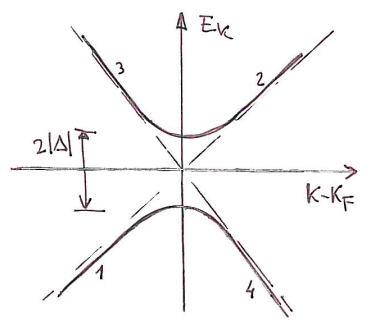
\includegraphics[width=0.4\linewidth]{Immagini - Capitolo 2/legge dispersione BCS.png}
    \caption{legge dispersione della teoria BCS dove le curve corrispondono all'energia di: 1. un quasi-elettrone con $k < k_F$; 2. un quasi-elettrone con $k > k_F$; una quasi-lacuna con $k < k_F$; 4. una quasi-lacuna con $k > k_F$.}
    \label{fig: legge dispersione BCS}
\end{figure}
Si intende adesso studiare l'andamento dei coefficienti
\begin{equation}
    |v_k|^2 = \frac{1}{2}\bigg(1 - \frac{\epsilon_k - \mu}{E_k}\bigg),\quad |u_k|^2 = \frac{1}{2}\bigg(1 + \frac{\epsilon_k - \mu}{E_k}\bigg),
\end{equation}
il cui andamento è mostrato in figura \ref{fig: coefficienti uk e vk}, dalla quale si nota che per $k - k_F \gg 0$ si hanno
\begin{align}
    \hatb_{k\upa} &= u_k^*\hatC_{k\upa} - v_k^*\hatCT_{-k\doa} \simeq u_k^*\hatC_{k\upa}, \\
    \hatbT_{-k\doa} &= v_k\hatC_{k\upa} + u_k\hatCT_{-k\doa} \simeq u_k\hatC_{-k\doa},
\end{align}
interpretati come gli operatori di distruzione e creazione di un quasi-elettrone rispettivamente, mentre per $k - k_F \ll 0$ si hanno
\begin{align}
    \hatb_{k\upa} &\simeq v_k^*\hatCT_{-k\doa}, \\
    \hatbT_{-k\doa} &\simeq v_k\hatC_{k\upa},
\end{align}
interpretati analogamente come gli operatori di distruzione e creazione di una quasi-lacuna rispettivamente. Quindi, gli operatori $\hatb$ e $\hatbT$ sono un mix di operatori di creazione di elettroni e lacune: gli stati che creano non sono né elettroni né lacune, ma una loro sovrapposizione quantistica. Dunque, i quasi-elettroni non hanno carica elettrica ben definita.
\begin{figure}[h]
    \centering
    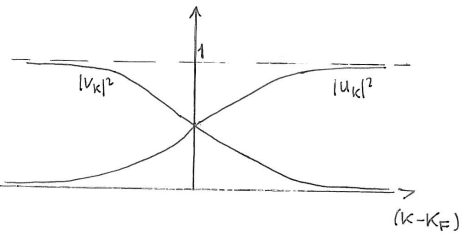
\includegraphics[width=0.5\linewidth]{Immagini - Capitolo 2/coefficienti uk e vk.png}
    \caption{andamento dei moduli $|u_k|^2$ e $|v_k|^2$ in funzione di $k - k_F$.}
    \label{fig: coefficienti uk e vk}
\end{figure}

Infatti, $u_k$ e $v_k$ hanno un'interpretazione probabilistica. Dato lo stato ad una particella
\begin{equation}
    \hatbT_{k\upa}\ket{\psi_{BCS}} = u_k\hatCT_{k\upa}\ket{\psi_{BCS}} - v_k\hatC_{-k\doa}\ket{\psi_{BCS}},
\end{equation}
il modulo $|u_k|^2$ è la probabilità di trovare un elettrone se si effettua una misura di carica, mentre $|v_k|^2$ è la probabilità di trovare una lacuna.
\begin{obs}
    Si ha un'interessante analogia con la fisica della particelle elementari. I mesoni $K^0$ e $\bar{K}^0$ sono formati da una coppia di quark $d\bar{s}$ e $s\bar{d}$, sono entrambi autostati dell'interazione forte e sono prodotti attraverso l'urto di protoni su un bersaglio, ma non sono autostati dell'interazione debole che non conserva la stranezza. Invece, si osservano oscillazioni tra uno stato e l'altro durante la propagazione.
\end{obs}

\subsection{Gap di energia}
A temperatura finita $T$, le quasi-particelle hanno numero di occupazione degli stati dato dalla distribuzione di Fermi-Dirac, ossia
\begin{equation}
    \vmedio{\hatbT_{k\upa}\hatb_{k\upa}}_T = \frac{1}{e^{\beta E_k} + 1} \equiv f(E_k)
\end{equation}
e di conseguenza
\begin{equation}
    \vmedio{\hatb_{-k\doa}\hatbT_{-k\doa}}_T = 1 - f(E_k).
\end{equation}
Per calcolare il valore di aspettazione $\vmedio{\hatC_{k\upa}\hatCT_{-k\doa}}_T$, si parte da
\begin{equation}
    \begin{pmatrix}
        \hatC_{k\upa} \\
        \hatCT_{-k\doa}
    \end{pmatrix} = U
    \begin{pmatrix}
        \hatb_{k\upa} \\
        \hatbT_{-k\doa}
    \end{pmatrix} = 
    \begin{pmatrix}
        u_k & v_k^* \\
        -v_k & u_k^*
    \end{pmatrix}
    \begin{pmatrix}
        \hatb_{k\upa} \\
        \hatbT_{-k\doa}
    \end{pmatrix},
\end{equation}
da cui si ha $\hatC_{-k\doa} = -v_k^*\hatbT_{k\upa} + u_k\hatb_{-k\doa}$, permettendo così di calcolare
\begin{equation}
    \begin{split}
        \vmedio{\hatC_{-k\doa}\hatC_{k\upa}}_T & =\vmedio{(-v_k^*\hatbT_{k\upa} + u_k\hatb_{-k\doa})(u_k\hatb_{k\upa} + v_k^*\hatbT_{-k\doa})}_T \\
        &= \vmedio{-v_k^*u_k\hatbT_{k\upa}\hatb_{k\upa} + u_kv_k^*\hatb_{-k\doa}\hatbT_{-k\doa}}_T \\
        &= v_k^*u_k[1 - 2f(E_k)].
    \end{split}
\end{equation}
Quindi, in funzione della temperatura il gap di energia è
\begin{equation}
    \Delta(T) = |g|\nsum_k\vmedio{\hatC_{k\upa}\hatC_{-k\doa}}_T = |g|\nsum_k u_kv_k^*[1 - 2f(E_k)],
\end{equation}
che generalizza il risultato per $T = \SI{0}{\kelvin}$. Dato che in prima approssimazione $u_kv_k^* = \Delta/2E_k$, allora
\begin{equation}
    \begin{split}
        \Delta(T) &= |g|\nsump{k}\frac{\Delta}{2E_k}\bigg(1 - \frac{2}{e^{\beta E_k} + 1}\bigg) \\
        &= |g|\nsump{k}\frac{\Delta}{2E_k}\frac{e^{\beta E_k/2} - e^{\beta E_k/2}}{e^{-\beta E_k/2} + e^{-\beta E_k/2}} \\
        &= g\nsump{k}\frac{\Delta}{2E_k}\tanh{\frac{E_k}{2kT}}.
    \end{split}
\end{equation}
Procedendo in modo simile al caso $T = \SI{0}{\kelvin}$, si ha
\begin{equation}
\label{eq: equazione del gap di energia BCS}
    \Lambda\int_0^{\hbar\omega_D}\frac{d\xi}{E(\xi)}\tanh{\frac{E(\xi)}{2kT}} = 1,\quad \xi \equiv \epsilon_k - \mu,
\end{equation}
dove $\Lambda = |g|D(\epsilon_F)$ e $E(\xi) = \sqrt{\xi^2 + |\Delta|^2}$.

\subsubsection{Dipendenza dalla temperatura}
Una stima della temperatura critica $T_c$ si ottiene sostituendo $T \to T_c$, per cui $\Delta(T_c) = 0$ e $E(\xi) = \xi$, nell'equazione \eqref{eq: equazione del gap di energia BCS}, ossia
\begin{equation}
    \Lambda\int_0^{\hbar\omega_D}\frac{d\xi}{\xi}\tanh{\frac{\xi}{2kT}} = \Lambda\int_0^{\beta\hbar\omega_D/2}\frac{dz}{z}\tanh{z},\quad z \equiv \frac{\xi}{2kT}.
\end{equation}
Per dare una stima dell'integrale 
\begin{equation}
    \int_0^y\frac{\tanh{z}}{z}\,dz,\quad y \gg 0,
\end{equation}
si integra per parti ottenendo
\begin{equation}
    \begin{split}
        \int_0^y\frac{\tanh{z}}{z}\,dz &= \log{(y)}\tanh{(y)} - \int_0^y\frac{\log{z}}{\cosh^2{z}}\,dz \\
        &\simeq \log{(y)} - \int_0^y\frac{\log{z}}{\cosh^2{z}}\,dz \\
        &= \log{(y)} - \bigg(-\gamma_E + \log{\frac{\pi}{4}}\bigg) \\
        &= \log{\bigg(\frac{\pi y}{4}e^{\gamma_E}\bigg)},
    \end{split}
\end{equation}
dove $\gamma_E = 0.577$ è la costante di Eulero-Mascheroni. Quindi, in questo caso
\begin{equation}
    \int_0^{\beta\hbar\omega_D/2}\frac{\tanh{z}}{z}\,dz \simeq \log{(A\hbar\omega_D\beta_C)},\quad A \equiv \frac{2e^{\gamma_E}}{\pi} \simeq 1.13,
\end{equation}
per cui 
\begin{equation}
    kT_c \simeq 1.13 \times (\hbar\omega_De^{-1/\Lambda}).
\end{equation}
Dunque, considerando il rapporto tra $\Delta(0) \simeq 2\hbar\omega_De^{-1/\Lambda}$ con $kT_c$ appena trovata si ha
\begin{equation}
    \frac{\Delta(0)}{kT_c} \simeq 1.76,
\end{equation}
che corrisponde ad una stima indipendente dal limite superiore $\hbar\omega_D$.
\begin{obs}
    Le quantità $\Delta(0)$ e $T_c$ possono essere misurate sperimentalmente in maniera indipendente. Il rapporto $\Delta(0)/kT_c$ misurato varia nel range $[1.6,2.3]$ nei superconduttori ``tradizionali'' con una distribuzione che si addensa intorno al valore teorico di 1.76.
\end{obs}
Per quanto riguarda $\Delta(T)$, questo può essere misurato numericamente dall'integrale
\begin{equation}
    \Lambda\int_0^{\hbar\omega_D}\frac{d\xi}{(\xi^2 + |\Delta|^2)^{1/2}}\tanh{\bigg[\frac{\beta}{2}(\xi^2 + |\Delta|^2)^{1/2}\bigg]} = 1.
\end{equation}
Per i superconduttori con $kT_c \ll \hbar\omega_D$, il rapporto $|\Delta(T)|/|\Delta(0)|$ è una funzione universale di $T/T_c$ che decresce monotonicamente da 1 a $T = \SI{0}{\kelvin}$ fino a zero per $T = T_c$. Intorno a $T = \SI{0}{\kelvin}$ la variazione è molto lenta poiché $e^{-\Delta/kT} \simeq 0$ e la tangente iperbolica è circa uno, quindi $\Delta(T)$ è circa costante fino a quando un grande numero di pseudo-particelle è stato eccitato termicamente. In particolare per $T \simeq T_c$, $\Delta(T)$ decresce a zero con tangente verticale 
\begin{equation}
    |\Delta(T)| \propto \bigg(1 - \frac{T}{T_c}\bigg)^{1/2}.
\end{equation}
\begin{obs}
    L'andamento con esponente critico pari ad $1/2$ è tipico di tutte le teorie di campo medio.
\end{obs}

\subsection{Densità degli stati}
Si può ottenere la densità degli stati $D_{BCS}$ nell'intorno dell'energia di Fermi come
\begin{equation}
    D_{BCS}(E)\,dE \simeq D(\epsilon_F)\,d(\epsilon - \mu) = D(\epsilon_F)\frac{d}{dE}(\epsilon - \mu)\,dE,
\end{equation}
dove 
\begin{equation}
    E(\epsilon - \mu) = 
    \begin{cases}
        -\sqrt{(\epsilon - \mu)^2 + |\Delta|^2},\quad \epsilon - \mu < 0 \\
        \sqrt{(\epsilon - \mu)^2 + |\Delta|^2},\quad \epsilon - \mu > 0
    \end{cases},
\end{equation}
la quale invertita restituisce
\begin{equation}
    \epsilon(E) - \mu = 
    \begin{cases}
        -\sqrt{E^2 - |\Delta|^2},\quad E < - |\Delta| \\
        0,\quad -|\Delta| \le E \le |\Delta| \\
        \sqrt{E^2 - |\Delta|^2},\quad E > |\Delta|
    \end{cases},
\end{equation}
la cui derivata è
\begin{equation}
    \frac{d}{dE}(\epsilon - \mu) = 
    \begin{cases}
        -\dfrac{E}{(E^2 - |\Delta|^2)^{1/2}},\quad E < - |\Delta| \\
        0,\quad -|\Delta| \le E \le |\Delta| \\
        \dfrac{E}{(E^2 - |\Delta|^2)^{1/2}},\quad E > |\Delta|
    \end{cases},
\end{equation}
dalla quale si può dedurre l'andamento della densità di stati $D_{BCS}$ mostrato in figura \ref{fig: densità di stati BCS}.
\begin{figure}[h]
    \centering
    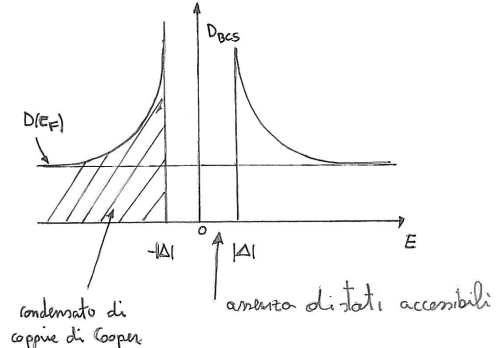
\includegraphics[width=0.4\linewidth]{Immagini - Capitolo 2/densità di stati BCS.png}
    \caption{andamento della densità di stati $D_{BCS}$ in funzione dell'energia.}
    \label{fig: densità di stati BCS}
\end{figure}

\subsection{scattering Andreev}
Un'ulteriore conferma dell'esistenza delle coppie di Cooper e del gap di energia si ottiene attraverso lo scattering di elettroni nel passaggio tra un metallo in regime classico e un altro in regime di superconduzione. Si consideri quindi un elettrone nel metallo in regime normale con impulso $\vk$, energia $\epsilon_k$ e terza componente di spin $\sigma$: se l'energia $\epsilon_k$ è minore di $|\Delta| + \epsilon_F$, allora l'elettrone non dovrebbe potersi propagare nel superconduttore, implicando quindi l'assenza di stati accessibili, e dovrebbe quindi essere riflesso all'interfaccia tra i due regimi, con il superconduttore che si comporta come un isolante. Si noti che nell'urto si conserva la carica elettrica, l'energia e lo spin, mentre non si conserva l'impulso.  
\begin{figure}[h]
    \centering
    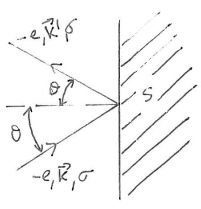
\includegraphics[width=0.3\linewidth]{Immagini - Capitolo 2/scattering C-SC.png}
    \caption{scattering di un elettrone all'interfaccia.}
    \label{fig: scattering C-SC}
\end{figure}

Tuttavia, Andreev osservò che nei superconduttori è possibile un altro processo: l'elettrone può combinarsi con un altro elettrone del metallo con impulso $\vk$ e spin $-\sigma$ per formare una coppia di Cooper che può propagarsi nel superconduttore sotto forma di supercorrente. Nel conduttore normale rimane però una lacuna con carica $e$, momento $\vk$, spin $\sigma$ e velocità di gruppo pari a 
\begin{equation}
    -\frac{\p}{\p\vk}\bigg(\frac{\hbar^2k^2}{2m} - \mu\bigg) = -\frac{\hbar^2}{2m}\vk.
\end{equation}
\begin{figure}[h]
    \centering
    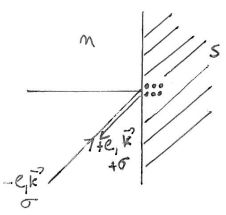
\includegraphics[width=0.3\linewidth]{Immagini - Capitolo 2/Andreev scattering.png}
    \caption{scattering Andreev.}
    \label{fig: Andreev scattering}
\end{figure}

Un'evidenza diretta di questo tipo di scattering si può ottenere iniettando una corrente all'interfaccia con un un superconduttore. Poiché la lacuna che torna indietro trasporta carica $e$, la corrente che passa nel superconduttore per effetto tunnel risulta essere il doppio rispetto a quella ottenibile per $\Delta = 0$ o per $\epsilon_k > |\Delta| + \epsilon_F$. La corrente trasportata dalla stato $\ket{\psi_{BCS}}$ è nulla; infatti calcolando il valore di aspettazione di $\hatJ_S$ si trova proprio
\begin{equation}
    \begin{split}
        \vJ_S = \mybrakett{\psi_{BCS}}{\hatJ_S}{\psi_{BCS}} &= \nsum_k\frac{\hbar}{2m}\vk(\vmedio{\hatN_{k\upa}}_{BCS} - \vmedio{\hatN_{-k\doa}}_{BCS}) \\
        &= \nsum_k\frac{\hbar}{m}\vk(|v_k|^2 - |v_k|^2) \\
        &= 0.
    \end{split}
\end{equation}
Bisognerebbe dimostrare che il gap di energia esiste anche quando le coppie di Cooper si muovono collettivamente, ossia per $\ket{\psi_{BCS}} \to \ket{\psi_{BCS},\vQ}$, dove 
\begin{equation}
    \ket{\psi_{BCS},\vQ} = \nprod_k(u_k^* + v_k^*\hatCT_{k + Q,\upa}\hatCT_{-k + Q,\doa})\kO.
\end{equation}
Questo stato corrisponde ad una soluzione consistente nel tempo di campo medio dell'hamiltoniana del modello BCS con 
\begin{align}
    \Delta Q &= |g|\nsum_k\vmedio{\hatC_{-k + Q,\doa}\hatC_{k + Q,\upa}}_{BCS}, \\
    \Delta^* Q &= |g|\nsum_k\vmedio{\hatCT_{-k + Q,\upa}\hatCT_{-k + Q,\doa}}_{BCS}.
\end{align}
L'hamiltoniana risultante può essere diagonalizzata e le eccitazioni di quasi-elettroni sopra questo stato possiedono una legge di dispersione ``deformata'', ma c'è ancora un gap di energia pari a 
\begin{equation}
    \Delta E \simeq 2|\Delta(0)| - \frac{2\hbar^2Qk_F}{m}.
\end{equation}
% \chapter{Effetto Hall quantistico}
L'effetto Hall classico fu scoperto nel 1879 da E. Hall studiando le proprietà dei conduttori in presenza di campi magnetici. Si consideri un conduttore lungo e sottile percorso da una corrente $I$ immerso in un campo magnetico $\vB$ perpendicolare al conduttore. A causa del campo $\vB$, gli elettroni percepiscono l'azione del campo magnetico tramite una forza di Lorentz che tende a farli deviare verso uno dei due bordi del conduttore. L'effetto di questo spostamento di cariche è la comparsa di una differenza di potenziale trasversale $V_H$, la quale è legata alla resistenza di Hall $R_H$ tramite la legge di Ohm
\begin{equation}
    R_H = \frac{V_H}{I},
\end{equation}
che a sua volta risulta essere proporzionale al campo magnetico che l'ha prodotta. Questo fenomeno ha avuto diverse applicazione pratiche ed in particolare è stato sfruttato per costruire sonde in grado di misurare campi magnetici attraverso semplici misure di tensione. Poco dopo la scoperta di Hall, von Klitzing notò che il comportamento di $R_H$ a temperature nell'ordine del Kelvin mostrava un comportamento radicalmente diverso da quello previsto classicamente. In queste condizioni, $R_H$ non varia più con continuità rispetto al campo magnetico applicato, ma assume soltanto un insieme discreto di valori, dati da
\begin{equation}
\label{eq: resistenza di Hall quantizzata}
    R_H = \frac{h}{\nu e^2} \equiv \frac{R_K}{\nu},\quad \nu \in \N,
\end{equation}
dove $R_K$ è la costante di von Klitzing. La spiegazione teorica di questo andamento, verificato sperimentalmente con precisioni dell'ordine di $10^{-9}$, è stata fornita da Laughlin poco dopo l'osservazione di von Klitzing. L'interpretazione dei dati sperimentali si basava sulle proprietà quantistiche universali dei singoli elettroni quando sono confinati a muoversi in due dimensioni e sono immersi in un campo magnetico perpendicolare alla direzione del loro moto. In queste condizioni, come già previsto da Landau, gli elettroni possiedono uno spettro discreto descritto da un opportuno oscillatore armonico, dove il numero di livelli completamente occupati è proprio il numero quantico $\nu$ presente nella relazione trovata da von Klitzing in equazione \eqref{eq: resistenza di Hall quantizzata}. In quegli stessi anni, Tsui, Stomer e Gossard scoprirono l'effetto Hall frazionario dove il numero intero $\nu$ viene sostituito da un numero frazionario $u$ nella relazione \eqref{eq: resistenza di Hall quantizzata}, ossia
\begin{equation}
    R_H = \frac{R_K}{u},\quad u \in \mathbb{Q}.
\end{equation}

La resistenza e la resistività sono legate dalla seconda legge di Ohm 
\begin{equation}
    R = \frac{\rho L}{A},
\end{equation}
dove $L$ è la lunghezza del conduttore e $A$ la sua sezione. In generale, considerando un ipercubo di lato $L$, ossia un cubo $D$-dimensionale, la resistenza è 
\begin{equation}
    R = \frac{\rho L}{L^{D - 1}} = \rho L^{2 - D}.
\end{equation}
Da questo si vede che il caso bidimensionale è peculiare dato che resistenza e resistività coincidono, in particolare $R$ è un invariante di scala e $e^2R/h$ è una quantità adimensionale. Questa proprietà è centrale per l'universalità dei risultati dato che non c'è bisogno di misurare le dimensioni del campione in modo estremamente preciso per ottenere la resistività alla precisione richiesta nel caso tridimensionale.

\section{Carica in un campo magnetico}
L'equazione del moto di un elettrone di carica $-e$, di massa $m$ e velocità $\vv$ soggetto alla forza di Lorentz dovuta ad un campo magnetico $\vB$ è
\begin{equation}
    m\frac{d\vv}{dt} = - e(\vv \times \vB).
\end{equation}
Se il campo magnetico è $\vB = B\,\hat{u}_z$ e la velocità iniziale è nel piano $(x,y)$, allora il moto è confinato in tale piano e il problema è bidimensionale. Date le coordinate $x_i \equiv (x_1,x_2) = (x,y)$ e le componenti della velocità $v_i \equiv (v_1,v_2) = (v_x,v_y)$ della particella si può scrivere l'equazione del moto come
\begin{equation}
    m\frac{dv_i}{dt} = -eB\epsilon_{ij}v_j = -m\omega_c\epsilon_{ij}v_j,
\end{equation}
dove $\omega_c = eB/m$ è la frequenza di ciclotrone, o di Larmor. Questa equazione si può riscrivere a sua volta come una derivata totale
\begin{equation}
    \frac{d}{dt}(p_i + m\omega_c\epsilon_{ij}x_j) = 0,
\end{equation}
da cui si deduce che il sistema possiede due costanti del moto 
\begin{equation}
    Q_i = p_i + m\omega_c\epsilon_{ij}x_j.
\end{equation}
Introducendo quindi la combinazione complessa $p = p_1 + ip_2$ si ha 
\begin{equation}
    \begin{cases}
        \dfrac{dp_1}{dt} = -\omega_cp_2 \\[2ex]
        i\dfrac{dp_2}{dt} = i\omega_cp_1
    \end{cases},
\end{equation}
che porta all'equazione differenziale 
\begin{equation}
\label{eq: equazione del moto di un carica in un campo B}
    \frac{dp}{dt} = i\omega_cp,
\end{equation}
la cui soluzione è
\begin{equation}
    p(t) = p_0e^{i\omega_c t},
\end{equation}
pertanto, dividendo per $m$ e integrando la velocità, si trova che la traiettoria della particella è 
\begin{equation}
    x(t) = x_1(t) + ix_2(t) = \frac{v_0}{i\omega_c}e^{i\omega_c t} + x_0 -   \frac{v_0}{i\omega_c}.
\end{equation}
Dunque, il moto è circolare uniforme con velocità angolare $\omega_c$ e raggio $R = v_0m/eB$.

Se ora al sistema si aggiunge un campo elettrico $\vE$ parallelo al piano $(x,y)$, l'equazione del moto diventa
\begin{equation}
    m\frac{d\vv}{dt} = -e(\vv \times \vB + \vE),
\end{equation}
o in forma complessa 
\begin{equation}
    \frac{dp}{dt} = i\omega_c\bigg(p - \frac{eE}{i\omega_c}\bigg),\quad E= E_1 + iE_2,
\end{equation}
la quale ponendo $\xi = p - eE/i\omega_c$, assume la medesima forma dell'equazione \eqref{eq: equazione del moto di un carica in un campo B} trovata prima; infatti si ha
\begin{equation}
    \frac{d\xi}{dt} = i\omega_c\xi,
\end{equation}
da cui si ricava immediatamente
\begin{equation}
\label{eq: velocità carica in campo EM}
    v(t) = v_0e^{i\omega_c t} + \frac{eE}{im\omega_c} = v_0e^{i\omega_c t} + \frac{E}{iB}.
\end{equation}
Il secondo termine in equazione \eqref{eq: velocità carica in campo EM} è chiamato ``velocità di trascinamento'' degli elettroni e indicato con $v_T$, la quale è dovuta alla presenza del campo elettrico $\vE$. Associata alla velocità di trascinamento è la densità di corrente
\begin{equation}
    \vJ = -en_e\vv_T = -\frac{en_e\vE}{iB},
\end{equation}
dove $n_e$ è la densità di elettroni, le cui componenti sono 
\begin{equation}
    J_x = -\frac{en_eE_y}{B},\quad J_y = \frac{en_eE_x}{B}.
\end{equation}
Quindi, la densità di corrente è perpendicolare al campo elettrico. Inoltre in generale, in un conduttore qualsiasi esiste una relazione lineare tra la densità di corrente e il campo elettrico della forma
\begin{equation}
    \begin{pmatrix}
        J_x \\
        J_y
    \end{pmatrix} = 
    \begin{pmatrix}
        \sigma_{xx} & \sigma_{xy} \\
        \sigma_{yx} & \sigma_{yy}
    \end{pmatrix}
    \begin{pmatrix}
        E_x \\
        E_y
    \end{pmatrix},
\end{equation}
oppure nella forma
\begin{equation}
    \begin{pmatrix}
        E_x \\
        E_y
    \end{pmatrix} = 
    \begin{pmatrix}
        \rho_{xx} & \rho_{xy} \\
        \rho_{yx} & \rho_{yy}
    \end{pmatrix}
    \begin{pmatrix}
        J_x \\
        J_y
    \end{pmatrix}.
\end{equation}
In particolare, per l'effetto Hall nel vuoto o in un conduttore ideale si ha che 
\begin{equation}
    \sigma_{xx} = \sigma_{yy} = 0,\quad \rho_{xx} = \rho_{yy} = 0, 
\end{equation}
mentre la conduttività di Hall è
\begin{equation}
    \sigma_H \equiv \sigma_{yx} = -\sigma_{xy} = \frac{n_ee}{B},
\end{equation}
tramite la quale si può scrivere la componente $x$ della densità di corrente $J$ come 
\begin{equation}
    J_x = -\sigma_H E_y.
\end{equation}
In un conduttore a forma di nastro di larghezza $L$, indicando con $V_y = -E_yL$ la differenza di potenziale tra i bordi e con $I_x = J_xL$ la corrente che scorre lungo l'asse $x$, si può scrivere
\begin{equation}
    \sigma_H = \frac{I_x}{V_y} = -\frac{\sigma_x}{E_y} = \frac{n_ee}{B},
\end{equation}
da cui 
\begin{equation}
\label{eq: resistenza di Hall classica}
    R_H = \frac{B}{n_ee}.
\end{equation}
Questo risultato si lega all'affermazione iniziale secondo cui la resistenza di Hall $R_H$ di un sistema classico tridimensionale cresce linearmente con l'intensità del campo magnetico che l'ha generata, a differenza di quanto accade in un sistema bidimensionale, come mostrato in figura \ref{fig: EH 3D vs 2D}.
\begin{figure}[h]
    \centering
    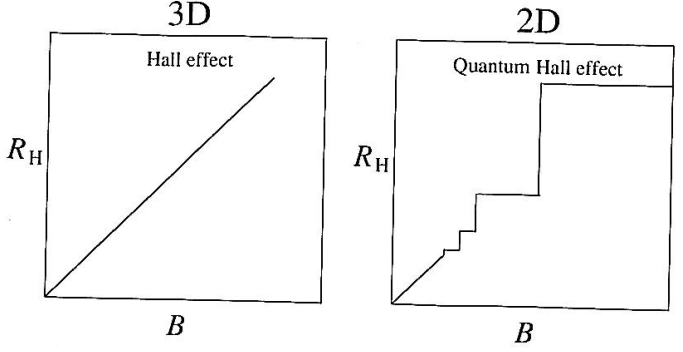
\includegraphics[width=0.6\linewidth]{Immagini - Capitolo 3/EH 3D vs 2D.png}
    \caption{differenza tra l'effetto Hall in tre dimensioni e in due dimensioni.}
    \label{fig: EH 3D vs 2D}
\end{figure}

\section{Livelli di Landau}
L'hamiltoniana per un elettrone non relativistico che si muove su un piano attraversato da un campo magnetico perpendicolare è
\begin{equation}
    \hatH = \frac{1}{2m}(\hatp + e\vA)^2.
\end{equation}
Se il campo magnetico è costante, allora vale che $\nabla \times \vA = B\,\hatz$, ossia che $\vA$ è lineare nelle coordinate $x$ ed $y$. Questo implica che l'hamiltoniana precedente è quella che descrive un oscillatore armonico e può pertanto essere diagonalizzata in modo esatto. Dato che l'equazione di Schr\"odinger è invariante per trasformazioni di gauge locali a causa della presenza del campo magnetico, è conveniente fissare il gauge, le scelte più usate sono:
\begin{enumerate}
    \item il gauge di Landau dove $\vA = B(-y,0,0)$ per geometrie a nastro;
    \item il gauge simmetrico dove $\vA = (B/2)(-y,x,0)$ per geometrie a disco.
\end{enumerate}

\subsection{Gauge di Landau}
In questo caso l'hamiltoniana non contiene termini dipendenti dalla coordinata $x$ e pertanto commuta con $p_x$. Questa proprietà implica che la funzione d'onda totale può essere fattorizzata come
\begin{equation}
    \eta(x,y) = \mathcal{N}e^{ik_xx}\phi(y).
\end{equation}
L'hamiltoniana del sistema può quindi essere scritta come
\begin{equation}
    \hatH = \frac{1}{2m}[p_y^2 + (\hbar k_x - eBy)^2].
\end{equation}
Conviene adesso introdurre le quantità
\begin{equation}
    l \equiv \sqrt{\frac{\hbar}{eB}},\quad y' \equiv \frac{y}{l} -lk_x,\quad p_y' \equiv \frac{lp_y}{\hbar},
\end{equation}
così da poter riscrivere l'hamiltoniana come
\begin{equation}
    \hatH = \hbar\omega_c\bigg(\frac{p_y'^2}{2}+ \frac{y'^2}{2}\bigg).
\end{equation}
Quindi, i livelli di energia quantizzati, detti livelli di Landau, sono 
\begin{equation}
    E_n = \hbar\omega_c\bigg(n + \frac{1}{2}\bigg),\quad n \in \N.
\end{equation}
In pratica, il continuo di livelli di energia presenti a $B = 0$, in presenza di un campo magnetico si combinano in modo tale da formare livelli di Landau degeneri, come mostrato in figura \ref{fig: livelli di Landau}. Se l'energia è quantizzata, un elettrone in un dato livello non può variare in modo continuo la sua energia cinetica, quindi la conservazione dell'energia lo vincola su linee equipotenziali. Si noti che l'energia non dipende da $k_x$, per cui autostati che differiscono solo in tale quantità e non in $n$ sono degeneri, mentre la posizione del centro dell'oscillatore dipende da $k_x$; infatti le autofunzioni sono
\begin{equation}
    \eta_{n,k_x} = \mathcal{N}e^{ik_xx}\exp{\bigg[-\frac{1}{2}\bigg(\frac{y}{l} - lk_x\bigg)^2\bigg]}H_x\bigg(\frac{y}{l} - lk_x\bigg),
\end{equation}
dove $H_n$ sono i polinomi di Hermite, localizzate attorno a $y_0(k_x) = l^2k_x \equiv y_0$.  
\begin{figure}[H]
    \centering
    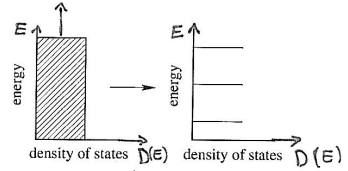
\includegraphics[width=0.5\linewidth]{Immagini - Capitolo 3/livelli di Landau.png}
    \caption{il mare di Fermi diviso in livelli di Landau equispaziati e degeneri in seguito all'applicazione del campo magnetico.}
    \label{fig: livelli di Landau}
\end{figure}

Quindi, lungo la direzione dell'asse $x$ si ha un'onda piana, mentre lungo la direzione dell'asse $y$ l'elettrone è localizzato e la traiettoria seguita è una linea retta centrata in $y_0(k_x)$. Cambiare valore di $k_x$ significa quindi cambiare traiettoria spostandosi verso il basso o verso l'alto, visualizzando così i momenti nello spazio delle coordinate. In particolare se si considera una geometria dove la direzione $x$ è periodica con lunghezza $L_x$, come ad esempio un cilindro la cui base ha lunghezza $L_x$, allora 
\begin{equation}
    k_x = \frac{2\pi}{L_x}n_x,\quad n_x \in \Z
\end{equation}
e la distanza tra i centri delle gaussiane, ossia la differenza tra le traiettorie seguite dagli elettroni, è 
\begin{equation}
    \Delta y_0 = \frac{2\pi l^2}{L_x}.
\end{equation}
Ricapitolando, introducendo un campo magnetico ortogonale alla geometria si è passati da un continuo di livelli energetici ad un insieme discreto di essi dato dai livelli di Landau, dove per $n = 0$ si ha il livello fondamentale associato all'oscillatore armonico. Quest'ultimo diventa infinitamente popolato se il volume della geometria è infinito, ma se questo non è il caso allora, dato che i momenti corrispondono a posizioni, si può dedurre che ogni livello di Landau non sia infinitamente popolato, ma sarà degenere e quindi dotato di un numero massimo di stati accessibili. Nel gauge di Landau gli orbitali degeneri sono etichettati dai numeri quantici $k_x$ e $n \in \N$. La degenerazione per unità di area è la stessa in ogni livello di Landau, ma dipende dal campo magnetico $\vB$. Per trovare la degenerazione si considera nuovamente la geometria data dal cilindro di dimensioni $L_x$ ed $L_y$, la cui periodicità permette di scrivere
\begin{equation}
    e^{ik_x(x + L_x)} = e^{ik_xx},
\end{equation}
per cui gli stati permessi sono dati da
\begin{equation}
    k_x = \frac{2\pi n_x}{L_x},\quad n_x \in \Z.
\end{equation}
Poiché il centro delle gaussiane è dato da $y_0$, solo gli stati con $0 < y_0 < L_y$ sono permessi, quindi per $y_0 = L_y$ si ha
\begin{equation}
    \frac{L_y}{l^2} = k_x^{(max)} = \frac{2\pi}{L_x}n_x^{(max)},
\end{equation}
ossia 
\begin{equation}
    n_x^{(max)} = \frac{L_yL_x}{2\pi l^2},
\end{equation}
che corrisponde quindi al numero massimo di stati nell'area $L_xL_y$. Pertanto, la degenerazione per unità di area è 
\begin{equation}
    \frac{n_x^{(max)}}{L_xL_y} = \frac{1}{2\pi l^2} = \frac{eB}{2\pi\hbar} = \frac{B}{\Phi_0}, 
\end{equation}
per cui
\begin{equation}
    n_x^{(max)} = \frac{\Phi}{\Phi_0}
\end{equation}
e in un livello di Landau ci può stare al più un elettrone per quanto di flusso di campo magnetico. Si può definire poi il fattore di riempimento come
\begin{equation}
    \nu = \frac{n_e\Phi_0}{B} = \frac{n_e\Phi_0L_xL_y}{BL_xL_y} \equiv \frac{\mathrm{\#\,di\,elettroni}}{\mathrm{\#\,di\,flussoni}}.
\end{equation}
Sostituendo $B = n_e\Phi_0/\nu = n_eh/e\nu$ nell'espressione di $R_H$ in \eqref{eq: resistenza di Hall classica} si trova la relazione di von Klitzing
\begin{equation}
    R_H = \frac{h}{\nu e^2}.
\end{equation}
I valori di $R_H$ osservati sperimentalmente in corrispondenza dei plateau sono 
\begin{equation}
    R_H = \frac{h}{ne^2},\quad n \in \N,
\end{equation}
come se il sistema, in corrispondenza dei plateau, avesse un fattore di riempimento $\nu$ intero anche se il campo magnetico sta variando. Le transizioni tra un plateau e l'altro avvengono in corrispondenza dei valori interi di $\nu$, mentre $\rho_{xx} \simeq 0$ diminuendo di un fattore $10^{-13}$ e presentando picchi in corrispondenza delle transizioni tra plateau.
\begin{figure}[h]
    \centering
    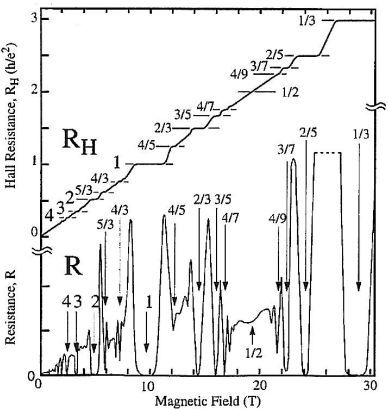
\includegraphics[width=0.49\linewidth]{Immagini - Capitolo 3/resistenze di Hall.png}
    \caption{valori sperimentali di $R_H$.}
    \label{fig: resistenze di Hall}
\end{figure}

\subsubsection{Splitting dei livelli energetici}
Quando il nastro è percorso da una corrente $I_x$ si manifesta una differenza di potenziale $\Delta V = -E_yL_y$ tra i due bordi e l'hamiltoniana del singolo elettrone nel gauge di Landau diventa
\begin{equation}
    \hatH =-\frac{\hbar^2}{2m}\frac{d^2}{dy^2} + \frac{m\omega^2_c}{2}(y - y_0)^2 + eyE_y,\quad y_0 = l^2k_x = \frac{\hbar k_x}{eB}.
\end{equation}
Questa continua ad essere l'hamiltoniana di un oscillatore armonico e ridefinendo il centro del sito di Landau come
\begin{equation}
    y_0 \to \tilde{y}_0 = y_0 - \frac{eE_y}{\omega_c^2 m}
\end{equation}
si ottiene
\begin{equation}
    \hatH = -\frac{\hbar^2}{2m}\frac{d^2}{dy^2} + \frac{m\omega_c^2}{2}(y_0 - \tilde{y}_0)^2 + eE_y\tilde{y}_0(k_x) + \frac{mE_y^2}{2B^2}.
\end{equation}
Lo spettro dei possibili livelli energetici risulta pertanto essere
\begin{equation}
\label{eq: legge dispersione livelli di Landau con campo E}
    E_{n,k_x} = \hbar\omega_c\bigg(n + \frac{1}{2}\bigg) + eE_y\tilde{y}_0(k_x) + \frac{mE_y^2}{2B^2}.
\end{equation}
Tale spettro ora dipende da entrambi i numeri quantici $n$ e $k_x$, mentre la presenza del campo elettrico $E_y$ rimuove completamente la degenerazione dei livelli energetici, infatti l'energia dipende esplicitamente dalla coordinata $\tilde{y}_0(k_x)$ del sito di Landau. Inoltre, per $B \gg E_y$, lo splitting dovuto al campo elettrico è trascurabile rispetto a $\hbar\omega_c = \hbar eB/m$ e quindi si trascura la possibilità di avere livelli di energia degeneri con numero quantico $n$ diverso. Tuttavia, nella geometria finita considerata bisogna tenere conto anche delle deformazione dei livelli ai bordi del sistema, come mostrato in figura \ref{fig: livelli energetici}.
\begin{figure}[h]
    \centering
    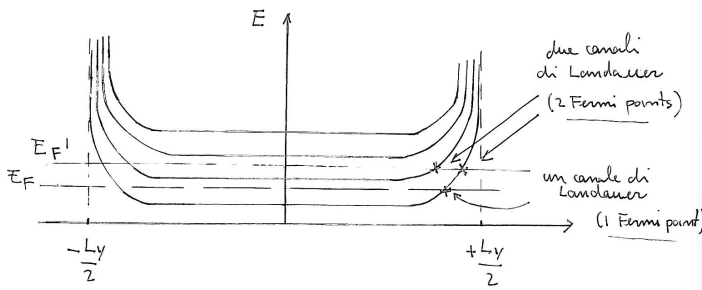
\includegraphics[width=0.7\linewidth]{Immagini - Capitolo 3/livelli energetici.png}
    \caption{livelli energetici per una geometria finita.}
    \label{fig: livelli energetici}
\end{figure}

Immaginando di avere il primo livello di Landau completamente riempito, gli unici elettroni che possono muoversi quando ricevono energia sono quelli ai bordi del conduttore. Questi elettroni possono muoversi praticamente lungo un'unica dimensione, dando luogo ad un tipo di conduzione detta ``balistica''. Per questo motivo la resistività $\rho_{xx}$ sui plateau è quasi nulla e le correnti possono resistere per solo per tempi sulla scala dei minuti, invece che per un tempo indefinito come accade per i superconduttori. Inoltre, la conduzione balistica differisce dalla superconduttività per l'assenza dell'effetto Meissner-Ochsenfeld.

Tuttavia, quanto detto non spiega la formazione dei plateau. Per spiegare la loro presenza si devono considerare le impurità nel reticolo, le quali contribuiscono allo splitting dei livelli di Landau anche in assenza del campo elettrico $E_y$, generando degli stati localizzati tra i livelli di Landau. Ad esempio, si supponga di avere il primo livello di Landau completamente riempito, gli elettroni anche avendo la possibilità di saltare al livello di Landau superiore, sono confinati dalle impurità al primo livello. Aumentando il fattore di riempimento, ad esempio diminuendo il campo magnetico $B$, gli elettroni migrano su stati localizzati e non partecipano alla corrente.

\subsubsection{Formula di von Klitzing}
A questo punto è possibile derivare la formula di von Klitzing per la corrente di Hall in presenza di impurità
\begin{equation}
\label{eq: formula di von Klitzing}
    I_H = \frac{e^2\nu}{h}V_H.
\end{equation}
Concentrandosi sul caso in cui $\nu = 1$, per $E_y = 0$, il campo magnetico agisce sugli elettroni facendogli seguire delle orbite circolari chiuse con frequenza $\omega_c$, per cui il trasporto di corrente avviene unicamente sui bordi del conduttore, come mostrato pittoricamente in figura \ref{fig: formula von Klitzing}. Inoltre, se $V_H = 0$, le due correnti sui bordi sono identiche in modulo e di verso opposto, confluendo quindi in una corrente netta nulla. 
\begin{figure}[h]
    \centering
    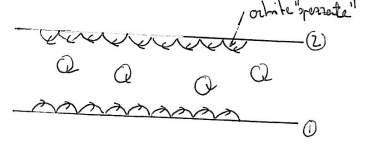
\includegraphics[width=0.5\linewidth]{Immagini - Capitolo 3/formula von Klitzing.png}
    \caption{trasporto di corrente in assenza di campo elettrico $E_y$.}
    \label{fig: formula von Klitzing}
\end{figure}

Invece, se $E_y = \mathrm{costante}$, allora la legge di dispersione per il primo livello di Landau, trovata in equazione \eqref{eq: legge dispersione livelli di Landau con campo E}, è
\begin{equation}
    \epsilon(k_x) = E_{0,k_x} = \frac{\hbar\omega_c}{2} + e\tilde{y}_0(k_x)E_y + \frac{mE_y^2}{2B^2}.
\end{equation}
Quindi, la velocità di gruppo nella direzione $x$ è
\begin{equation}
    v_{k_x} = \frac{1}{\hbar}\frac{\p\epsilon(k_x)}{\p k_x} = \frac{eE_y}{\hbar}\frac{\p\tilde{y}_0(k_x)}{\p k_x} = \frac{eE_yl^2}{\hbar} = \frac{E_y}{B},
\end{equation}
che coincide proprio con la velocità di trascinamento $v_T \equiv E_y/B$ ed pertanto indipendente da $k_x$.

Considerando adesso il caso in cui, a causa della presenza di impurità, il campo elettrico è una funzione $E_y \equiv E_y(y)$, la legge di dispersione restituisce
\begin{equation}
    \epsilon(k_x) = \frac{\hbar\omega_c}{2} + e\tilde{y}_0E_y(\tilde{y}_0) + \frac{mE_y(\tilde{y}_0)^2}{2B^2},\quad \tilde{y}_0 \equiv \tilde{y}_0(k_x),
\end{equation}
mentre la velocità di gruppo è nuovamente data da
\begin{equation}
    v_{k_x} = \frac{1}{\hbar}\frac{\p\epsilon(k_x)}{\p k_x},
\end{equation}
con la quale si può calcolare la corrente che percorre il dispositivo
\begin{equation}
    I_H = -e\int\frac{dk_x}{2\pi}\frac{1}{\hbar}\frac{\p\epsilon(k_x)}{\p k_x}\eta_{k_x}.
\end{equation}
Se lo stato è completamente occupato, allora $\eta_{k_x}$, che corrisponde alla probabilità che lo stato $k_x$ sia occupato, è pari ad uno, per cui la corrente risulta essere
\begin{equation}
    I_H = -\frac{e}{h}[\mu(L_y) - \mu(0)] = \frac{e^2}{h}V_H.
\end{equation}
Quindi, nel caso di $\nu$ generico, $\eta_{k_x}$ viene sostituito da $\nu \eta_{k_x}$ e la corrente assume la forma
\begin{equation}
    I_H = \frac{e^2\nu}{h}V_H,
\end{equation}
che è proprio la formula di von Klitzing per la corrente di Hall in equazione \eqref{eq: formula di von Klitzing}.

\subsubsection{Gedanken experiment di Laughlin}
Si consideri un dispositivo di Hall a forma di disco bucato al centro. Si supponga di instaurare un flusso di campo magnetico $\Phi(t)$ attraverso il foro del dispositivo, il quale viene incrementato adiabaticamente nel tempo da 0 a $\Phi_0$. Per la legge di Faraday, un cambiamento del flusso di campo magnetico induce un campo elettrico dato da
\begin{equation}
    \oint_\Gamma d\vl \cdot \vE = -\frac{\p\Phi(t)}{\p t},
\end{equation}
dove l'integrale viene considerato su un cammino chiuso che circonda il foro del disco. Dato che non si ha dissipazione e che $\sigma_{xx} = \sigma_{yy} = \rho_{xx} = \rho_{yy} = 0$, il campo elettrico induce una densità di corrente
\begin{equation}
    \vE = \rho_{xy}(\vJ \times \hatz) = (\rho_{xy}J_y,0,0),
\end{equation}
quindi la legge di Faraday si riscrive come
\begin{equation}
    \rho_{xy}\oint_\Gamma (\hatz \cdot d\vl) \cdot \vJ = -\frac{d\Phi(t)}{dt},
\end{equation}
dove l'integrale nel membro di sinistra rappresenta la corrente totale che fluisce all'interno della regione delimitata dal percorso $\Gamma$, potendo quindi scrivere
\begin{equation}
    \rho_{xy}\frac{dQ(t)}{dt} = -\frac{d\Phi(t)}{dt},
\end{equation}
la quale integrata tra $t = 0$ dove $\Phi = 0$ e $t'$ dove $\Phi = \Phi_0$ restituisce
\begin{equation}
    \rho_{xy}Q = -\Phi_0.
\end{equation}
Quindi, la carica può essere scritta in funzione del fattore di riempimento
\begin{equation}
    Q = \sigma_{xy}\Phi_0 = \frac{h}{e}\sigma_{xy} = \nu e,
\end{equation}
dove si è usato che sui plateau $\sigma_{xy} = \nu e^2/h$. Dunque, a causa di una variazione del campo magnetico all'interno del sistema, una corrente radiale trasporta una carica $Q = \nu e$ verso il bordo interno del dispositivo, come mostrato in figura \ref{fig: Gedanken experiment}. Poiché l'inserimento di un flusso di campo magnetico ha un costo energetico pari a $\Delta U = \nu eV_H$, il sistema si trova in uno stato eccitato. Nel caso dell'effetto Hall frazionario, questo evidenzia l'esistenza di quasi-particelle con carica frazionaria. 
\begin{figure}[h]
    \centering
    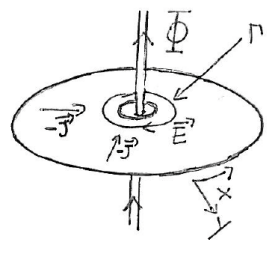
\includegraphics[width=0.3\linewidth]{Immagini - Capitolo 3/Gedanken experiment.png}
    \caption{dispositivo di Hall immerso in un campo magnetico.}
    \label{fig: Gedanken experiment}
\end{figure}

\subsection{Gauge simmetrico}
In questo caso, introducendo direttamente le variabili adimensionali
\begin{equation}
    l \equiv \sqrt{\frac{\hbar}{eB}},\quad y' \equiv \frac{y}{l},\quad x' \equiv \frac{x}{l},\quad p'_{x,y} = \frac{lp_{x,y}}{\hbar},
\end{equation}
l'hamiltoniana risulta essere
\begin{equation}
    \hatH' \equiv \frac{\hatH}{\hbar\omega_c} = \frac{1}{2}\bigg[\bigg(-i\frac{\p}{\p x'} - \frac{y'}{2}\bigg)^2 + \bigg(-i\frac{\p}{\p y'} + \frac{x'}{2}\bigg)^2\bigg].
\end{equation}
Definendo adesso le variabili complesse
\begin{equation}
    z = x' - iy' = re^{-i\theta},\quad \zbar  = x' + iy' = re^{i\theta},
\end{equation}
le derivate che compaiono nell'espressione di $\hatH'$ diventano
\begin{equation}
    \frac{\p}{\p x'} = \frac{\p}{\p z} + \frac{\p}{\p \zbar },\quad \frac{\p}{\p y'} = -i\bigg(\frac{\p}{\p z} - \frac{\p}{\p \zbar }\bigg).
\end{equation}
\begin{notz}
    La ragione per cui si usa questa convenzione per $z$ è che le funzioni d'onda dello stato fondamentale di Landau dipendono solo da $z$, a parte un fattore gaussiano $\exp{(-z\zbar /4)}$.
\end{notz}
Riscrivendo adesso l'hamiltoniana come
\begin{equation}
    \begin{split}
        \hatH' &= \frac{1}{2} + \frac{1}{2}\bigg[\bigg(-i\frac{\p}{\p y'} + \frac{x'}{2}\bigg) - i\bigg(-i\frac{\p}{\p x'} - \frac{y'}{2}\bigg)\bigg] \\
        &\times\bigg[\bigg(-i\frac{\p}{\p y'} + \frac{x'}{2}\bigg) + i\bigg(-i\frac{\p}{\p x'} - \frac{y'}{2}\bigg)\bigg],
    \end{split}
\end{equation}
si possono definire gli operatori 
\begin{align}
    \frac{1}{\sqrt{2}}\bigg[\bigg(-i\frac{\p}{\p y'} + \frac{x'}{2}\bigg) - i\bigg(-i\frac{\p}{\p x'} - \frac{y'}{2}\bigg)\bigg] &= \frac{1}{\sqrt{2}}\bigg(-2\frac{\p}{\p z} + \frac{\zbar }{2}\bigg) \equiv \hataT, \\
    \frac{1}{\sqrt{2}}\bigg[\bigg(-i\frac{\p}{\p y'} + \frac{x'}{2}\bigg) + i\bigg(-i\frac{\p}{\p x'} - \frac{y'}{2}\bigg)\bigg] &= \frac{1}{\sqrt{2}}\bigg(2\frac{\p}{\p \zbar} + \frac{z}{2}\bigg) \equiv \hata,
\end{align}
tali da soddisfare la relazione di commutazione 
\begin{equation}
    \comm{\hata}{\hataT} = 1,
\end{equation}
così da rendere l'hamiltoniana della forma
\begin{equation}
    \hatH' = \hataT\hata + \frac{1}{2}.
\end{equation}
Definendo lo stato di vuoto $\kO$ come $\hata\kO = 0$, si introduce la funzione d'onda $\eta_0(z,\zbar )$ cosicché 
\begin{equation}
\label{eq: funzione d'onda gauge simmetrico}
    \frac{1}{\sqrt{2}}\bigg(2\frac{\p}{\p \zbar } + \frac{z}{2}\bigg)\eta_0(z,\zbar ) = 0,
\end{equation}
che è equivalente a quanto detto nel formalismo di Schr\"odinger. Risolvendo poi l'equazione appena trovata
\begin{align}
    \frac{\p}{\p\zbar }\eta_0(z,\zbar) &= -\frac{z}{4}\eta_0(z,\zbar) \\
    \frac{\p}{\p\zbar}\log{\eta_0(z,\zbar)} &= -\frac{z}{4},
\end{align}
si ottiene
\begin{equation}
    \eta_0(z,\zbar) = \frac{1}{\sqrt{2\pi}}P(z)e^{-z\zbar/4},
\end{equation}
dove $P(z)$ è una funzione generica analitica in $z \in \C$, cioè una funzione non singolare intera che è possibile sviluppare sulla base $\{z^m\}$ con $m \ge 0$. A tale scopo, si osserva che gli operatori 
\begin{equation}
    \hatbT = \frac{1}{\sqrt{2}}\bigg(-2\frac{\p}{\p\zbar} + \frac{z}{2} \bigg),\quad \hatb = \frac{1}{\sqrt{2}}\bigg(2\frac{\p}{\p z} + \frac{\zbar}{2} \bigg) 
\end{equation}
commutano con gli operatori $\hata$, $\hataT$ e l'hamiltoniana $\hatH'$, per cui 
\begin{equation}
    \comm{\hatb}{\hatbT} = 1.
\end{equation}
Pertanto, si introduce lo stato annichilato simultaneamente dagli operatori $\hatb$ e $\hata$ tale per cui $\hatb\ket{0,0} = 0$, ossia che abbia la forma trovata in equazione \eqref{eq: funzione d'onda gauge simmetrico}, perciò
\begin{equation}
    \frac{1}{\sqrt{2}}\bigg(2\frac{\p}{\p z} + \frac{\zbar}{2} \bigg)\eta_{0,0}(z,\zbar) = \bigg[\frac{1}{\sqrt{2}}\bigg(\frac{\zbar}{2} - \frac{\zbar}{2}\bigg)P(z) + \sqrt{2}\frac{\p P(z)}{\p z}\bigg]\frac{e^{-z\zbar/4}}{\sqrt{2\pi}} = 0,
\end{equation}
da cui si trova che $P(z) = 1$. Analogamente, l'operatore $\hatbT$ agisce su questo stato come $\hatbT\ket{0,0} = \ket{0,1}$, per cui
\begin{equation}
    -\frac{1}{\sqrt{2}}\bigg(2\frac{\p}{\p\zbar} + \frac{z}{2} \bigg)\eta_{0,0}(z,\zbar) = \frac{z}{\sqrt{2}}\eta_{0,0}(z,\zbar) \equiv \eta_{0,1}(z,\zbar),
\end{equation}
o più in generale come
\begin{equation}
    \frac{(\hatbT)^m}{\sqrt{m!}}\ket{0,0} = \ket{0,m},
\end{equation}
per cui 
\begin{equation}
    \frac{(\hatbT)^m}{\sqrt{m!}}\eta_{0,0}(z,\zbar) = \frac{z^me^{-z\zbar/4}}{\sqrt{2\pi2^mm!}} = \eta_{0,m}(z,\zbar).
\end{equation}
Nel caso del gauge di Landau, si era trovato che per una geometria periodica le traiettorie riempiono lo spazio ma sono spaziate per il principio di esclusione di Pauli, similmente per una geometria a disco si possono graficare le traiettorie semi-classiche per ogni $n$ corrispondenti ai picchi della gaussiana, dove il raggio di ogni orbita è proporzionale ad $m^{1/2}$. La componente del momento angolare nella direzione $z$ è 
\begin{equation}
    \hatL' \equiv \frac{\hatL}{\hbar} = -i\frac{\p}{\p\theta},
\end{equation}
per cui
\begin{equation}
    z\frac{\p}{\p z} - \zbar\frac{\p}{\p \zbar} = \hatbT\hatb - \hataT\hata,
\end{equation}
dove il termine a primo membro corrisponde alla differenza tra il momento angolare trasportato dalla parte olomorfa, $\p/\p z$, e quello trasportato dalla parte anti-olomorfa, $\p/\p\zbar$, mentre nel termine a secondo membro $\hatbT\hatb$ aumenta $n$ ed $m$ mentre $\hataT\hata$ aumenta $n$ ma diminuisce $m$. Dato che gli operatori $\hatH$ e $\hatL$ commutano possono essere diagonalizzati simultaneamente. Gli stati costruiti sono autostati di $\hatL'$ con autovalore $-m$ con $m = [-n,\infty) \subset \Z$, ad esempio
\begin{equation}
    \hatL'\eta_{0,m}(z\zbar) = N\bigg(\zbar\frac{\p}{\p\zbar} - z\frac{\p}{\p z}\bigg)(z^me^{-z\zbar/4}) = -m\eta_{0,m}(z\zbar).
\end{equation}
Analogamente, gli autostati di $\hatH'$ per $n$ ed $m$ generici sono
\begin{equation}
    \ket{n,m} = \frac{(\hatbT)^{n+m}(\hataT)^n}{\sqrt{(n + m)!}\sqrt{n!}}\ket{0,0}
\end{equation}
con 
\begin{equation}
    \eta_{n,m}(z,\zbar) = N_{n,m}\bigg(\frac{z}{2} - 2\frac{\p}{\p\zbar}\bigg)^{n + m}\bigg(\frac{\zbar}{2} - 2\frac{\p}{\p z}\bigg)^ne^{-z\zbar/4}
\end{equation}
dove
\begin{equation}
    N_{n,m} = \frac{1}{\sqrt{2\pi 2^{m + 2n}n!(n + m)!}},
\end{equation}
che può essere riscritta in forma più compatta come
\begin{equation}
    \eta_{n,m}(z\zbar) = \frac{(-1)^n}{\sqrt{2\pi}}\sqrt{\frac{n!}{2^m(n + m)!}}e^{-r^2/4}z^mL_n^m\bigg(\frac{r^2}{4}\bigg),\quad r^2 \equiv z\zbar,
\end{equation}
dove $L^m_n$ sono i polinomi di Laguerre, la quale è effettivamente soluzione dell'oscillatore armonico in due dimensioni. 

Ignorando i fattori di normalizzazoine nel seguito, si consideri adesso la base di funzioni d'onda con momento angolare definito 
\begin{equation}
\label{eq: funzione d'onda singolo elettrico gauge simmetrico}
    \psi_m = z^me^{-|z|^2/4},\quad |\psi_m|^2 = |z|^{2m}e^{-|z|^2/2},
\end{equation}
il cui massimo di probabilità si può trovare ponendo
\begin{equation}
    \frac{\p|\psi_m|^2}{\p|z|} = (2m|z|^{2m - 1} - |z|^{2m + 1})e^{-|z|^2/2} = 0,
\end{equation}
da cui si trova che il raggio delle traiettorie è dato da 
\begin{equation}
    |z| = \sqrt{2m},
\end{equation}
per cui l'area delimitata da essa è 
\begin{equation}
    r^2\pi = 2ml^2\pi\quad\Longrightarrow\quad m = \frac{\pi r^2}{2\pi l^2},\quad |z| = \frac{r}{l}.
\end{equation}
Quindi, la traiettoria semi-classica dell'elettrone racchiude $m$ quanti di flusso $\Phi_0$; pertanto, all'elettrone dopo aver completato un'orbita viene associata una fase pari al numero di quanti di flusso $\Phi_0$ contenuti nell'area delimitata da tale orbita. Perciò la monodromia di $\psi_m$ è data dalla relazione
\begin{equation}
    \psi_m(z e^{2i\pi}) = \psi_m(z)e^{2i\pi m}.
\end{equation}
Nel gauge simmetrico le funzioni d'onda a singolo elettrone hanno la forma trovata in equazione \eqref{eq: funzione d'onda singolo elettrico gauge simmetrico}. Si tenta ora di costruire le funzioni d'onda per uno stato ad $N$ particelle. Per farlo si può usare il determinante di Slater così da avere una funzione d'onda totale, ad esempio per gli stati a due e tre particelle si hanno
\begin{equation}
    \begin{split}
        \psi^{(2)} &= 
        \begin{vmatrix}
            1 & 1 \\
            z_1 & z_2
        \end{vmatrix} 
        e^{-|z_1|^2/4}e^{-|z_2|^2/4} \\
        &= -(z_1 - z_2)\exp{\bigg[-\frac{1}{4}(|z_1|^2 + |z_2|^2)\bigg]},
    \end{split}
\end{equation}
\begin{equation}
    \begin{split}
        \psi^{(3)} &= 
        \begin{vmatrix}
            1 & 1 & 1 \\
            z_1 & z_2 & z_3 \\
            z_1^2 & z_2^2 & z_3^2
        \end{vmatrix} 
        e^{-|z_1|^2/4}e^{-|z_2|^2/4}e^{-|z_3|^2/4} \\
        &= [(z_2z_3^2 - z_3z_2^2) - (z_1z_3^2 - z_3z_1^2) + (z_1z_2^2 - z_2z_1^2)] \\
        &\times\exp{\bigg[-\frac{1}{4}(|z_1|^2 + |z_2|^2 + |z_3|^2)\bigg]} \\
        &= -\prod_{i<j}^3(z_i - z_j)\exp{\bigg[-\frac{1}{4}(|z_1|^2 + |z_2|^2 + |z_3|^2)\bigg]},
    \end{split}
\end{equation}
e così via. Quindi, in generale lo stato ad $N$ particelle è dato da
\begin{equation}
\label{eq: funzione d'onda stato ad N particelle gauge simmetrico}
    \psi \equiv \psi^{(N)} = \prod_{i<j}^N(z_i - z_j)\exp{\bigg(-\frac{1}{4}\nsum_j|z_j|^2\bigg)}
\end{equation}
e la probabilità non normalizzata per le particelle nel primo livello di Landau è
\begin{equation}
\label{eq: densità funzione d'onda stato ad N particelle gauge simmetrico}
    |\psi|^2 = \prod_{i<j}^N|z_i - z_j|^2\exp{\bigg(-\frac{1}{2}\nsum_j|z_j|^2\bigg)}.
\end{equation}
Quest'ultimo oggetto è molto complesso da trattare, è chiaro che il termine polinomiale diventi molto articolato se le particelle rimangono ben distanziate; d'altra parte il termine esponenziale tende a non farle disperdere troppo sfavorendo valori di $|z|$ troppo grandi. Per questo è difficile anche trovare una risposta a quesiti semplici come l'uniformità della densità delle particelle. Per risolvere il problema, Laughlin ha sviluppato un'analogia con la fisica del plasma che riesce a chiarire molte delle proprietà della funzione d'onda in equazione \eqref{eq: funzione d'onda stato ad N particelle gauge simmetrico}.

\subsubsection{Plasma interpretation}
Si introduce un funzione di partizione ipotetica 
\begin{equation}
    Z = \bigg(\int d^2z_1 \cdots \int d^2z_N\bigg)|\psi|^2,
\end{equation}
corrispondente alla funzione di partizione di un problema classico di meccanica statistica con peso di Boltzmann 
\begin{equation}
    |\psi|^2 = e^{-zU_C/\beta},
\end{equation}
dove
\begin{equation}
    U_C = \beta^2\sum_{i < j}^N(-\log{|z_i - z_j|}) + \frac{\beta}{4}\sum_{k=1}^N|z_k|^2 \equiv \beta^2U_{int}^{(N)} + \frac{\beta}{4}U_B^{(N)}.
\end{equation}
Il potenziale $U_C$ corrisponde all'energia potenziale di un plasma classico 2-dimensionale composto da particelle di carica $\beta$ in un background uniforme ``neutrilazzante''. Si può quindi utilizzare l'intuito per i sistemi classici di plasma per studiare la proprietà di $|\psi|^2$. Tramite le coordinate complesse $z$ e $\zbar$, il potenziale elettrostatico può essere riassunto nella forma
\begin{equation}
    \phi(z,\zbar) = -Q\log{\frac{|z|l}{r_0}}
\end{equation}
che, fissando $r_0 = l$ diventa
\begin{equation}
    \phi(z,\zbar) = -Q\log{|z|}.
\end{equation}
L'energia di interazione tra due cariche $Q$ poste a distanza $|z|$ è
\begin{equation}
    U^{(2)}_{int} = -Q^2\log{|z|},
\end{equation}
si vede quindi che il termine 
\begin{equation}
    U^{(N)}_{int} = \beta^2\sum_{i < j}^N(-\log{|z_i - z_j|})
\end{equation}
può essere interpretato come l'energia potenziale di interazione di un gas di $N$ particelle in due dimensioni con carica $\beta$. Bisogna però sempre tenere conto del fatto che non c'è nessun potenziale logaritmico nell'hamiltoniana di cui $\psi$ è soluzione. Per comprendere l'analogia con il plasma, si deve considerare che la carica $Q$ è data da
\begin{equation}
    \int d\vSigma \cdot \vE = 4\pi Q,
\end{equation}
poiché l'area della sfera è $4\pi r^2$, si ottengono
\begin{equation}
    \vE(\vr) = \frac{Q}{r^2}\hatr,\quad \phi(\vr) = \frac{Q}{r},
\end{equation}
tali per cui 
\begin{equation}
    \nabla \cdot \vE = -\nabla^2\phi.
\end{equation}
In due dimensioni 
\begin{equation}
    \int d\vSigma \cdot \vE = 2\pi Q,
\end{equation}
quindi si hanno 
\begin{equation}
    \vE(\vr) = \frac{Q}{r}\hatr,\quad \phi(\vr) = -Q\log{\frac{r}{r_0}}.
\end{equation}
Per comprendere il significato del termine $U_B^{(N)}$ si nota che 
\begin{equation}
    l\bigg(\frac{\p}{\p x} + i\frac{\p}{\p y}\bigg) = 2\frac{\p}{\p z},\quad l\bigg(\frac{\p}{\p x} - i\frac{\p}{\p y}\bigg) = 2\frac{\p}{\p \zbar},
\end{equation}
ossia
\begin{equation}
    \nabla^2 = \frac{\p^2}{\p x^2} + \frac{\p^2}{\p y^2} = \frac{4}{l^2}\frac{\p}{\p z}\frac{\p}{\p \zbar}.
\end{equation}
Quindi, si ha la relazione
\begin{equation}
    -\nabla^2 \frac{|z|^2}{4} = -\frac{1}{l^2}\frac{\p}{\p z}\frac{\p}{\p \zbar}(z\zbar) = -\frac{1}{l^2} = 2\pi\rho_B\quad\Longrightarrow\quad \rho_B = \frac{1}{2\pi l^2}.
\end{equation}
Tale equazione può essere interpretata come l'equazione di Poisson associata ad una distribuzione omogenea di carica $\rho_B$, dove
\begin{equation}
    \phi_B(z,\zbar) = \frac{|z|^2}{4}
\end{equation}
corrisponde al potenziale associato a questa distribuzione di carica. L'energia potenziale di una particella con carica $Q$ a distanza $|z|$ dal centro del sistema è
\begin{equation}
    U_B^{(1)} = \frac{Q|z|^2}{4}.
\end{equation}
Il termine $U^{(N)}_B$ in $U_C$ 
\begin{equation}
    U_B^{(N)} = \frac{\beta}{4}\nsum_k|z_k|^2
\end{equation}
rappresenta quindi l'energia potenziale elettrostatica legata alla presenza di un background con densità di carica $\rho_B$. Supponendo ora di aggiungere un quanto di flusso $\Phi_0$ adiabaticamente a $z = 0$, come nel gedanken experiment di Laughlin, si ha
\begin{equation}
    \psi_m(z) \to \psi_{m + 1}(z) = z^{m + 1}e^{|z|^2/4},
\end{equation}
ossia l'elettrone si è spostato sull'orbita successiva. Per il sistema a molti elettroni questo corrisponde a
\begin{equation}
    \psi^{(N)} = \prod_{i < j}^N(z_i - z_j)\exp{\bigg({-\frac{1}{4}\nsum_k|z_k|^2}\bigg)} \to \bigg(\nprod_kz_k\bigg)\psi^{(N)}.
\end{equation}

\section{Effetto Hall frazionario}
Con la scoperta dell'effetto Hall frazionario con fattore di riempimento $\nu = 1/3$, Laughlin intuì immediatamente che altri valori di $\beta$ erano possibili ed erano in grado di descrivere il fluido quantistico di Hall a $\nu = 1/\beta$ con $\beta \in \N$ dispari. La funzione d'onda corrispondente è
\begin{equation}
    \psi_\beta^{(N)} = \prod_{i < j}^N(z_i - z_j)^\beta\exp{\bigg(-\frac{1}{4}\nsum_k|z_k|^2\bigg)}
\end{equation}
ed è completamente antisimmetrica e sviluppabile sulla base $\{z^me^{-|z|^2/4}\}^{\otimes N}$ delle funzioni d'onda del primo livello di Landau; in particolare, il termine $\prod_{i < j}(z_i - z_j)^\beta$ contiene solo fattori olomorfi $\{(z_i)^k\}$ con $k \in [0,N] \subset \N$. Si supponga di voler determinare la funzione d'onda a due elettroni con momento angolare del centro di massa $M$ e momento angolare relativo $m$. Trascurando il mixing dei livelli di Landau per $n \ge 1$, la funziona d'onda deve essere sviluppabile sulla base 
\begin{equation}
    \{z_1^{m_1}e^{-|z_1|^2/4}\} \otimes \{z_2^{m_2}e^{-|z_2|^2/4}\},
\end{equation}
ossia la parte esponenziale deve essere olomorfa in $z_1$ e $z_2$, per cui 
\begin{equation}
    \psi^{(2)} = F(z_1,z_2)\exp{\bigg[-\frac{1}{4}(|z_1|^2 + |z_2|^2)\bigg]}.
\end{equation}
La funzione d'onda deve essere separabile in una parte corrispondente al moto del centro di massa e in una parte legata al moto relativo, quindi
\begin{equation}
    \psi^{(2)}_{m,M} = f(z_1 - z_2)g(z_1 + z_2)\exp{\bigg[-\frac{1}{4}(|z_1|^2 + |z_2|^2)\bigg]}.
\end{equation}
Considerando la simmetria per rotazione 
\begin{equation}
    \begin{cases}
        f[(z_1 - z_2)e^{2i\pi}] = e^{2i\pi m}f(z_1 - z_2) \\
        g[(z_1 + z_2)e^{2i\pi}] = e^{2i\pi M}g(z_1 + z_2)
    \end{cases},
\end{equation}
l'unica soluzione possibile indipendentemente dal tipo di potenziale di interazione è
\begin{equation}
    \psi^{(2)}_{m,M} = (z_1 - z_2)^m(z_1 + z_2)^M\exp{\bigg[-\frac{1}{4}(|z_1|^2 + |z_2|^2)\bigg]},
\end{equation}
dove $m \in \N$ dispari. Considerando anche l'interazione a due corpi, l'energia corrispondente a tale stato è 
\begin{equation}
    E = \frac{\mybrakett{m,M}{\hatH_1 + \hatH_2 + \hatV_{12}}{m,M}}{\mybraket{m,M}{m,M}} = \hbar\omega_c + \frac{\mybrakett{m,M}{\hatV_{12}}{m,M}}{\mybraket{m,M}{m,M}},
\end{equation}
nel caso di interazione coulombiana
\begin{equation}
    E_{12}(m,M) = E_{12}(m) = e^2k\frac{\mybrakett{m,M}{|z|^{-1}}{m,M}}{\mybraket{m,M}{m,M}} = \frac{\sqrt{2}(2m)!}{2^{2m + 1}(m!)^2}e^2k,
\end{equation}
dove $k$ è la costante di Coulomb; in particolare, per $m \gg 1$ e usando l'approssimazione di Stirling il risultato è $E_{12}(m) \simeq 1/\sqrt{2m}$ dove $\sqrt{2m}$ è il raggio dell'orbita contenente $m$ quanti di flusso $\Phi_0$. Questo dimostra che i livelli energetici sono quantizzati come se fossero\ stati legati. In assenza di campo magnetico, la forza coulombiana repulsiva tende a far allontanare gli elettroni che perdono energia potenziale acquistando energia cinetica. In presenza di campo magnetico invece l'energia cinetica è quantizzata ed è pari a $\hbar\omega_c/2$ per ogni elettrone nel primo livello di Landau. Pertanto, gli elettroni non possono allontanarsi e formano stati legati con energia di legame $E_{12}$ positiva. In queste condizioni, a fissato fattore di riempimento $1/\beta$, il sistema presenta un gap di energia. Si consideri ad esempio $\nu = 1/3$, tutte le coppie di elettroni possiedono momento angolare relativo $m = 3$, per cui
\begin{equation}
    \psi^{(N)} = \prod_{i < j}^N(z_i - z_j)^3\exp{\bigg(-\frac{1}{4}\nsum_k|z_k|^2\bigg)}
\end{equation}
e uno stato eccitato corrisponderebbe quindi ad una transizione; ad esempio, $m = 3 \to m = 5$ per una coppia di elettroni $(12)$. Tuttavia, a fissato fattore di riempimento, un'altra coppia di elettroni deve transire $m'=3 \to m'=1$. Inoltre, poiché
\begin{align}
    \Delta E &= \Delta E_{12}(3 \to 5) + \Delta E_{12}(3 \to 1) \\
    &= E_{12}(5) - E_{12}(3) + E_{12}(1) - E_{12}(3) \\
    &= \frac{31\sqrt{2\pi}}{512}e^2k,
\end{align}
si ha una gap di energia $E_{12} > 0$ positivo e lo stato con $\nu = 1/3$ corrisponde quindi ad un fluido incomprimibile. La presenza di tale gap, come nel caso con $\nu = 1$, è cruciale per avere $\rho_{xx} = \sigma_{xx} = \rho_{yy} = \sigma_{yy} = 0$. 

\end{document}